\documentclass[10pt,twocolumn,letterpaper]{article}

\usepackage{iccv}

% This is roughly version 1.1 of vcl-shortcuts, circa Dec 2016.
% Put together by Vladlen Koltun

\usepackage{times}
\usepackage{epsfig}
\usepackage{graphicx}
\usepackage{float}
\usepackage{wrapfig}
\usepackage{amsmath,amssymb,amsthm}
\usepackage{algorithm,algorithmicx,algpseudocode}
\usepackage{bm,xspace}
\usepackage{comment}
\usepackage{verbatim}
\usepackage{multirow}
\usepackage{balance}
\usepackage{url}
\usepackage{booktabs}
\usepackage{etoolbox,siunitx}
\usepackage{calc}
\usepackage{pifont,hologo}

%Set up nice tables using the tabular package
%Make \toprule and \bottomrule thicker than \midrule
\setlength\heavyrulewidth{0.10em}
\setlength\lightrulewidth{0.05em}
\setlength\cmidrulewidth{0.03em}
\newcommand{\ra}[1]{\renewcommand{\arraystretch}{#1}}

%Set up the siunitx package, particularly for using the S column type in tables
\usepackage[super]{nth}
\usepackage{nicefrac}
\sisetup{detect-weight=true,detect-inline-weight=math}
\sisetup{quotient-mode = fraction}
\sisetup{fraction-function = \nicefrac}
\robustify\bfseries


%Known issue: the following shortcuts override \gg, \ll\, and \tt, which are existing LaTeX commands. Use \ggreater and \llesser, defined below, instead of \gg and \ll. Use \texttt{} instead of \tt.
\def\aa{\mathbf{a}}
\def\bb{\mathbf{b}}
\def\cc{\mathbf{c}}
\def\dd{\mathbf{d}}
\def\ee{\mathbf{e}}
\def\ff{\mathbf{f}}
\def\gg{\mathbf{g}}
\def\hh{\mathbf{h}}
\def\ii{\mathbf{i}}
\def\jj{\mathbf{j}}
\def\kk{\mathbf{k}}
\def\ll{\mathbf{l}}
\def\mm{\mathbf{m}}
\def\nn{\mathbf{n}}
\def\oo{\mathbf{o}}
\def\pp{\mathbf{p}}
\def\qq{\mathbf{q}}
\def\rr{\mathbf{r}}
\def\ss{\mathbf{s}}
\def\tt{\mathbf{t}}
\def\uu{\mathbf{u}}
\def\vv{\mathbf{v}}
\def\ww{\mathbf{w}}
\def\xx{\mathbf{x}}
\def\yy{\mathbf{y}}
\def\zz{\mathbf{z}}

\def\AA{\mathbf{A}}
\def\BB{\mathbf{B}}
\def\CC{\mathbf{C}}
\def\DD{\mathbf{D}}
\def\EE{\mathbf{E}}
\def\FF{\mathbf{F}}
\def\GG{\mathbf{G}}
\def\HH{\mathbf{H}}
\def\II{\mathbf{I}}
\def\JJ{\mathbf{J}}
\def\KK{\mathbf{K}}
\def\LL{\mathbf{L}}
\def\MM{\mathbf{M}}
\def\NN{\mathbf{N}}
\def\OO{\mathbf{O}}
\def\PP{\mathbf{P}}
\def\QQ{\mathbf{Q}}
\def\RR{\mathbf{R}}
\def\SS{\mathbf{S}}
\def\TT{\mathbf{T}}
\def\UU{\mathbf{U}}
\def\VV{\mathbf{V}}
\def\WW{\mathbf{W}}
\def\XX{\mathbf{X}}
\def\YY{\mathbf{Y}}
\def\ZZ{\mathbf{Z}}

\def\aA{\mathcal{A}}
\def\bB{\mathcal{B}}
\def\cC{\mathcal{C}}
\def\dD{\mathcal{D}}
\def\eE{\mathcal{E}}
\def\fF{\mathcal{F}}
\def\gG{\mathcal{G}}
\def\hH{\mathcal{H}}
\def\iI{\mathcal{I}}
\def\jJ{\mathcal{J}}
\def\kK{\mathcal{K}}
\def\lL{\mathcal{L}}
\def\mM{\mathcal{M}}
\def\nN{\mathcal{N}}
\def\oO{\mathcal{O}}
\def\pP{\mathcal{P}}
\def\qQ{\mathcal{Q}}
\def\rR{\mathcal{R}}
\def\sS{\mathcal{S}}
\def\tT{\mathcal{T}}
\def\uU{\mathcal{U}}
\def\vV{\mathcal{V}}
\def\wW{\mathcal{W}}
\def\xX{\mathcal{X}}
\def\yY{\mathcal{Y}}
\def\zZ{\mathcal{Z}}

\def\Ae{\mathbb{A}}
\def\Be{\mathbb{B}}
\def\Ce{\mathbb{C}}
\def\Le{\mathbb{L}}
\def\Ne{\mathbb{N}}
\def\Pe{\mathbb{P}}
\def\Qe{\mathbb{Q}}
\def\Re{\mathbb{R}}
\def\Se{\mathbb{S}}
\def\Te{\mathbb{T}}
\def\Xe{\mathbb{X}}
\def\Ye{\mathbb{Y}}
\def\Ze{\mathbb{Z}}

\def\btheta{{\bm\theta}}
\def\bzeta{{\bm\zeta}}
\def\bmu{{\bm\mu}}
\def\bZero{\mathbf{0}}
\def\bOne{\mathbf{1}}

\DeclareMathOperator*{\argmax}{arg\,max}
\DeclareMathOperator*{\argmin}{arg\,min}
\DeclareMathOperator*{\minimize}{minimize}
\DeclareMathOperator*{\maximize}{minimize}

\DeclareMathOperator{\sign}{sign}
\DeclareMathOperator{\rank}{rank}
\DeclareMathOperator{\trace}{tr}
\DeclareMathOperator{\diag}{diag}
\DeclareMathOperator{\diam}{diam}

\def\eps{\varepsilon}
\def\vphi{\varphi}
\def\vsigma{\varsigma}

\def\trans{^{\top}}
\def\deg{^{\circ}}

\def\th{^{\textnormal{th}}}
\def\st{^{\textnormal{st}}}
\def\nd{^{\textnormal{nd}}}

%\ggreater and \llesser replace \gg and \ll, which have been overridden
\newcommand\ggreater{\mathbin{>\!\!\!>}}
\newcommand\llesser{\mathbin{<\!\!\!<}}

%Checkmark and cross symbols for tables
\newcommand{\YesV}{\ding{51}}%
\newcommand{\NoX}{\ding{55}}%

%Use @ instead of , in long numbers in math mode. For example, use $10@000$ rather than $10,000$.
\DeclareMathSymbol{@}{\mathord}{letters}{"3B}

\newcommand\paren[1]{\left(#1\right)}
\newcommand\abs[1]{\left\lvert#1\right\rvert}
\newcommand\norm[1]{\left\lVert#1\right\rVert}
\newcommand\tuple[1]{\left\langle#1\right\rangle}
\newcommand\inner[2]{\langle #1, #2 \rangle}

%Use \timess instead of \times in the main lines of equations, but not in superscripts or subscripts. Use the regular \times in superscripts or subscripts.
\newcommand\timess{\mathbin{\!\times\!}}

%Known issue: \nicebar is not nice in PNAS format, use \bar if submitting to PNAS.
\newcommand\nicebar[1]{\mkern 4mu\overline{\mkern-4mu#1}}

%Replace ``\yourname" and ``Name" with your name
\newcommand\yourname[1]{\textcolor{blue}{Name says: #1}}
\newcommand\vladlen[1]{\textcolor{blue}{Vladlen says: #1}}

%Paragraph heading with customizable vertical spacing. Modify the length inside \vspace to expand or contract the vertical offset preceding a new paragraph heading.
\newcommand\mypara[1]{\vspace{1mm}\noindent\textbf{#1}}

%Orient text vertically. Useful for tables and figures.
\def\rot#1{\rotatebox{90}{#1}}

%I use the self-indulgent \LaTeX operator mostly to illustrate an issue and a useful trick. The issue is that LaTeX operators eat the space that follows them, so if they occur in the middle of a sentence they eliminate the space separating the following word. But you can't just insert a space will-nilly (e.g., \LaTeX\ or \LaTeX~) because if the operator is followed by a punctuation mark then there shouldn't be a space. One solution is to write \LaTeX{}, which does the right thing but is easy to forget. The alternative, demonstrated here, is to define an operator with a name that ends with the forward slash. This also does the right thing and looks sufficiently distinctive to be memorable.
\def\latex/{\LaTeX}
\def\bibtex/{\hologo{BibTeX}}

%Miscellaneous \latex/ tips:
% To create an invisible character, use the \phantom command or its relatives: http://tex.stackexchange.com/questions/4519/how-do-i-create-an-invisible-character


% Include other packages here, before hyperref.

% If you comment hyperref and then uncomment it, you should delete
% egpaper.aux before re-running latex.  (Or just hit 'q' on the first latex
% run, let it finish, and you should be clear).
\usepackage[pagebackref=true,breaklinks=true,letterpaper=true,colorlinks,bookmarks=false]{hyperref}

\iccvfinalcopy % *** Uncomment this line for the final submission

\def\iccvPaperID{253} % *** Enter the ICCV Paper ID here
\def\httilde{\mbox{\tt\raisebox{-.5ex}{\symbol{126}}}}

% Pages are numbered in submission mode, and unnumbered in camera-ready
\ificcvfinal\pagestyle{empty}\fi
\begin{document}

%%%%%%%%% TITLE
\title{Photographic Image Synthesis with Cascaded Refinement Networks}

\setcounter{footnote}{1}

\author{Qifeng Chen\thanks{Intel Labs}~~\thanks{Stanford University}
%\\
%\textsuperscript{1}Stanford University
% For a paper whose authors are all at the same institution,
% omit the following lines up until the closing ``}''.
% Additional authors and addresses can be added with ``\and'',
% just like the second author.
% To save space, use either the email address or home page, not both
\and
Vladlen Koltun\footnotemark[2]
%\\
%\textsuperscript{2}Intel Labs
}

\makeatletter
\g@addto@macro\@maketitle{
  \begin{figure}[H]
  \setlength{\linewidth}{\textwidth}
  \setlength{\hsize}{\textwidth}
  \vspace{-7mm}
  \centering
 	\begin{tabular}{@{}c@{\hspace{1mm}}c@{}}
  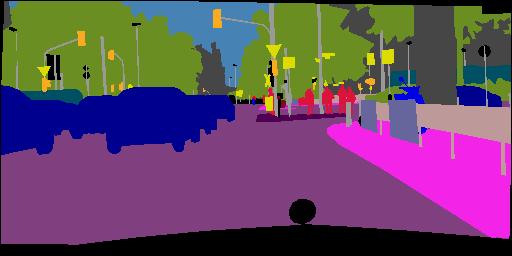
\includegraphics[width=0.493\textwidth]{figures/Label_000027.png} &
  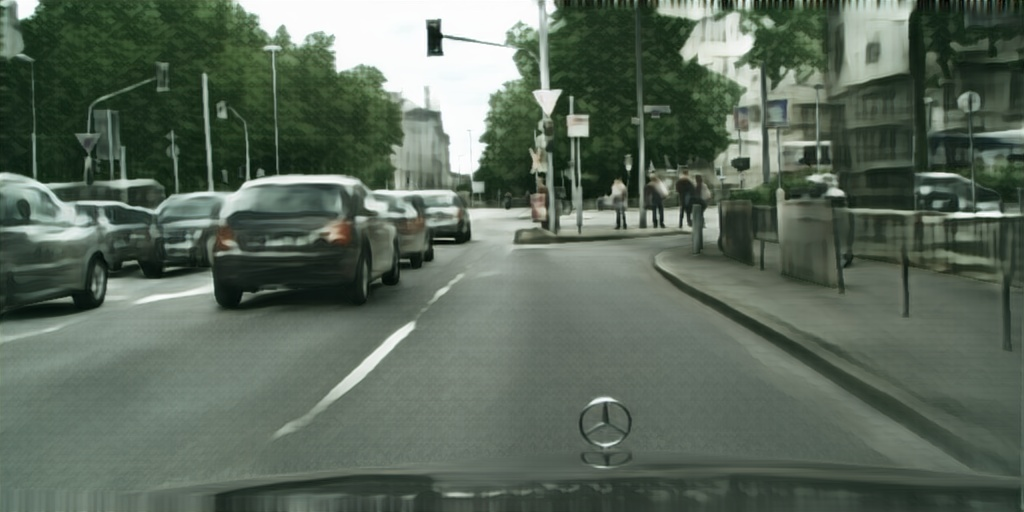
\includegraphics[width=0.493\textwidth]{figures/Ours_000027.jpg}\vspace{0mm}\\
  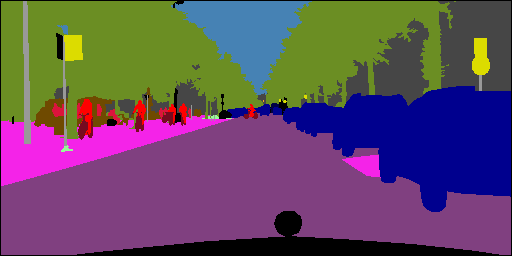
\includegraphics[width=0.493\textwidth]{figures/Label_000338.png} &
  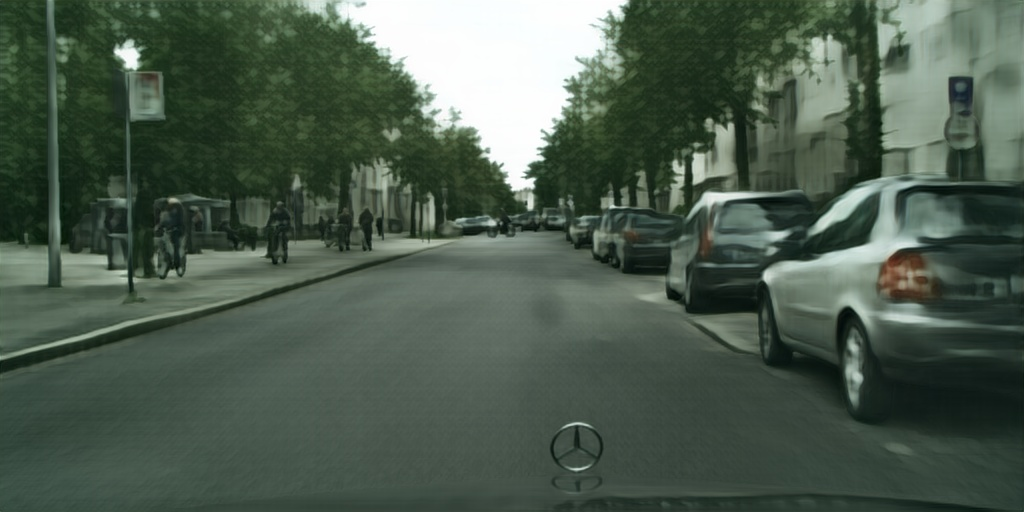
\includegraphics[width=0.493\textwidth]{figures/Ours_000338.jpg}\\
\small (a) Input semantic layouts & \small (b) Synthesized images
 	\end{tabular}
  \vspace{1mm}
  \caption{Given a pixelwise semantic layout, the presented model synthesizes an image that conforms to this layout. (a) Semantic layouts from the Cityscapes dataset of urban scenes; semantic classes are coded by color. (b) Images synthesized by our model for these layouts. The layouts shown here and throughout the paper are from the validation set and depict scenes from new cities that were never seen during training. Best viewed on the screen.}
  \label{fig:teaser}
%  \vspace{2mm}
  \end{figure}
}
\makeatother

\maketitle
%\thispagestyle{empty}

%%%%%%%%% ABSTRACT
\begin{abstract}
We present an approach to synthesizing photographic images conditioned on semantic layouts. Given a semantic label map, our approach produces an image with photographic appearance that conforms to the input layout. The approach thus functions as a rendering engine that takes a two-dimensional semantic specification of the scene and produces a corresponding photographic image. Unlike recent and contemporaneous work, our approach does not rely on adversarial training. We show that photographic images can be synthesized from semantic layouts by a single feedforward network with appropriate structure, trained end-to-end with a direct regression objective. The presented approach scales seamlessly to high resolutions; we demonstrate this by synthesizing photographic images at 2-megapixel resolution, the full resolution of our training data. Extensive perceptual experiments on datasets of outdoor and indoor scenes demonstrate that images synthesized by the presented approach are considerably more realistic than alternative approaches.
\end{abstract}

%%%%%%%%% BODY TEXT

\section{Introduction}
\label{sec:introduction}
\section{Introduction}

Locating visual landmarks, such as human body joints \cite{toshev2014deeppose} and facial key points \cite{xiong2013supervised}, is an important yet challenging problem. The stacked U-Nets, {\it e.g.} hourglasses (HGs) \cite{newell2016stacked}, are widely used in landmark localization. Generally speaking, their success can be attributed to design patterns: 1) within each U-Net, connect the top-down and bottom-up feature blocks to encourage gradient flow; and 2) stack multiple U-Nets in a cascade to refine prediction stage by stage.

However, the shortcut connection exists only ``locally'' inside each U-Net \cite{ronneberger2015u}. There is no ``global'' connection across U-Nets except the cascade. Blocks in different U-Nets cannot share features, which may impede the information flow and lead to redundant parameters.

We propose densely connected U-Nets (DU-Net) to address this issue. The key idea is to directly connect blocks of the same semantic meanings, {\it i.e.} having the same resolution in either top-down or bottom-up context, from any U-Net to all subsequent U-Nets. Please refer to Fig. \ref{fig:framework} for an illustration. The dense connectivity is similar to DenseNet \cite{huang2016densely} but generalizing the design philosophy from feature to semantic level. It encourages information flow as well as feature reuse ``globally'' across the stacked U-Nets, yielding improved localization accuracy. 

Yet there are critical issues in designing DU-Net: 1) The number of parameters would have a quadratic growth since $n$ stacked U-Nets could generate $O(n^2)$ connections. 2) A naive implementation may allocate new memory for every connection, making the training highly expensive and limiting the maximum depth of DU-Nets. 

% The training would be extremely memory expensive since a naive implementation has to make a copy of every connected feature for network forward and back propagation.  



\begin{figure*}[t!]
\centering
  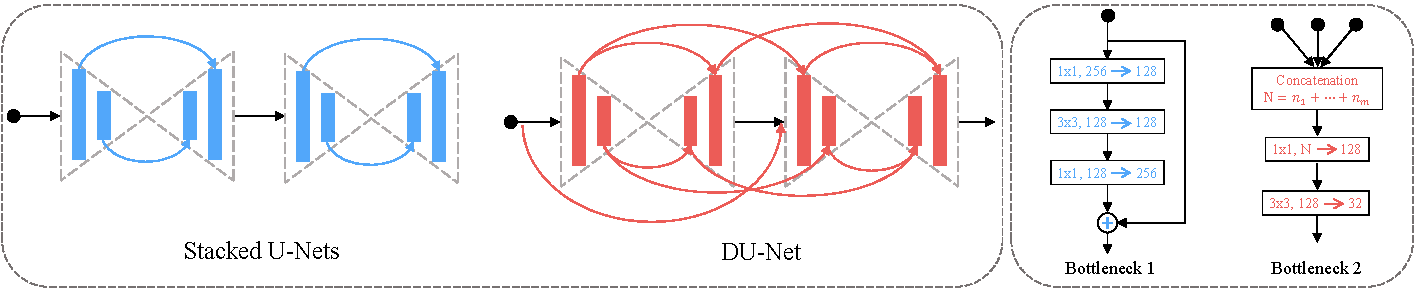
\includegraphics[width=1.0\linewidth]{figures/framework-cropped.pdf}
\caption{Illustration of stacked U-Nets and DU-Net. Stacked U-Nets has skip connections only within each U-Net. In contrast, DU-Net also connects blocks with the same semantic meanings across different U-Nets. The feature reuse could significantly reduce the size of bottleneck in each block, as shown in the right figure. Consequently, with the same number of U-Nets, DU-Net has only 30\% parameters of stacked U-Nets.}
\label{fig:framework}
\end{figure*}

% 
Our solution to those efficiency issues is threefold. {\bf First}, instead of connecting all stacked U-Nets, we only connect a U-Net to its $K$ successors. We name it as the $order$-$K$ connectivity, which aims to balance the fitting accuracy and parameter efficiency by cutting off long-distance connections. {\bf Second}, we employ a memory-efficient implementation in training. The key idea is to reuse a pre-allocated memory so all connected blocks could share the same memory. Compared with the naive implementation, this strategy makes it possible to train a very deep DU-Net (actually, $2\times$ deeper). {\bf Third}, to further improve the efficiency, we investigate an iterative design that may reduce the model size to one half. More specifically, the output of the first pass of the DU-Net is used as the input of the second pass, where detection or regression loss is applied as supervision. 

% %G%
% In view of deploying our approach on mobile devices, we further attempt to quantize weights, inputs, and gradients of DU-Net to low bit-width discrete values. This not only decreases the high precision operations but also shrinks the memory usage during training. By network quantization, the size of trained model can also be largely compressed.
% %G%
Besides shrinking the number of network parameters, we also study to further quantize each parameter. This motivates from the ubiquitous mobile applications. Although current mobile devices could carry models of dozens of MBs, deploying such networks requires high-end GPUs. However, quantized models could be accelerated by some specifically designed low-cost hardwares. Beyond only deploying models on mobile devices \cite{li2017deeprebirth}, training deep neural networks on distributed mobile devices emerges recently \cite{mcmahan2016communication}. To this end, we also try to quantize not only the model parameters but also its inputs (intermediate features) and gradients in training. This is the first attempt to investigate training landmark localizers using quantized inputs and gradients.


In summary, our key contributions are:
\begin{itemize}
    \item To the best of our knowledge, we are the first to propose quantized densely connected U-Nets for visual landmark localization, which largely improves the information flow and feature reuse at the semantic level.
    \item We propose the $order$-$K$ connectivity to balance accuracy and efficiency. It decreases the growth of model size from quadratic to linear by removing trivial connections. Experiments show it could reduce $\sim$70\% parameters of state-of-the-art landmark localizers.
    \item Very deep U-Nets can be trained using a memory-efficient implementation, where pre-allocated memory is reused by all connected blocks.
    \item We further investigate an iterative refinement that may cut down half of the model size, by forwarding DU-Net twice using either detection or regression supervision.
    %G%
    \item Different from previous efforts of quantizing only the model parameters, we are the first to quantize their inputs and gradients for better training efficiency on landmark localization tasks. By choosing appropriate quantization bit-widths for weights, inputs and gradients, quantized DU-Net achieves $\sim$75\% training memory saving with comparable performance. 
    %G%
    \item Exhaustive experiments are performed to validate DU-Net in different aspects. In both human pose estimation and face alignment, DU-Net demonstrates comparable localization accuracy and use $\sim$2\% model size compared with state-of-the-art methods.
\end{itemize}

% We are the first to deploy network quantization for better training efficiency on localization tasks. By choosing appropriate quantization bit-widths for weights, inputs and gradients, quantized DU-Net achieves at least 32$\times$ memory saving with comparable performance to the-state-of-art approaches. 


%The landmark localization such as human pose estimation \cite{toshev2014deeppose,newell2016stacked,wei2016convolutional}, facial landmark localization \cite{xiong2013supervised,zhang2014facial,sagonas2013300}, etc, plays an important role in the higher-level image understanding. The Convolutional Neural Networks (CNNs) have dominated this field, among which recent architecture of stacked hourglasses \cite{newell2016stacked}, a variant of the U-Net \cite{ronneberger2015unet}, becomes a standard solution. The skip connections between top-down and bottom-up blocks within a U-Net could preserve the spatial information and increase the gradient flow. With multiple U-Nets stacked together, the prediction could be refined stage by stage. However, the connections are only within each U-Net of the stacked hourglasses and no explicit connections exist between U-Nets, which may impede the information flow across them. And the blocks with the same semantics in different U-Nets cannot share features, leading to many redundant parameters. 

% Its success attributes to three key factors: repeated top-down, bottom-up inferences, intermediate supervisions and residual bottlenecks \cite{}. 

% The multiple stage top-down and bottom-up processing could better integrate both the local and global visual contexts into the final prediction. The intermediate supervision and residual bottlenecks, on the other hand, could alleviate the gradient vanish problem in deep networks.
%In this paper, we propose to densely connect stacked U-Nets by linking blocks with the same semantics in different U-Nets. We refer to this architecture as {\it Dense U-Nets}. The blocks in a U-Net could get direct inputs from its connected blocks in all preceding U-Nets, making the information flow more efficiently among the U-Nets. The feature reuse at each resolution could reduce the parameters in each block. The dense connectivity in our Dense U-Nets is different from that of DenseNet \cite{huang2016densely}. More specifically, layers only within each single block of the DenseNet are connected. In contrast, we connect blocks lying across the whole Dense U-Nets and connections of hierarchical blocks are mixed together. An illustration is given in Figure \ref{fig:framework}. We name it as the {\it global dense connectivity} to differentiate from the local one in the DenseNet.

% Besides, features in the Dense U-Nets are fused by the concatenation which could facilitate the information flow compared with the summation operation in the stacked hourglasses.

% Although the dense connectivity in our Dense U-Nets is similar with that of DenseNet \cite{}, 
% More recently, the DenseNet \cite{} achieves superior image classification performance over the ResNet \cite{} in terms of both the accuracy and model size, which benefits from the dense connections between layers. Its key insight is the feature reuse between layers of the same resolutions. The dense connectivity in the DenseNet, existing within one block, is local. By extending this principle, we propose a global dense connectivity, in contrast to the local connectivity in \cite{}, that blocks at the same locations of different U-Nets are connected. Hence, we refer to this architecture as {\it Dense U-Nets}. To our best knowledge, we are the first to generalize the local dense connectivity into the stacked U-Nets. 
% The global dense connectivity could make it easier to train much deeper stacked U-Nets.

% This motivates us to replace the residual modules  in the stacked hourglasses with the dense connected layers. However, this dense connectivity exists only locally within a contiguous  block in which all feature maps have the same spatial resolution. A U-Net, on the other hand, consists of a sequence of top-down and bottom-up blocks. A straight way is to turn each block into a dense block with multiple layers. However, this would sacrifice the spirit of stacked hourglasses that multiple stacked hourglasses outperform a single hourglass with multiple layers in each block.

% In order to integrate the structure of stacked U-Nets together with the idea of dense connectivity, we propose a global dense connectivity, in contrast to the local connectivity in \cite{}, that blocks at the same locations of different U-Nets are connected. Hence, we refer to this architecture as {\it Dense U-Nets}. The connected layers in the Dense U-Nets distribute along the whole network rather than in local continuous blocks. Compared with the local residual modules in the stacked hourglasses, the global dense connections could significantly facilitate the gradient to flow across stacked U-Nets.

%In practice, the Dense U-Nets have the efficiency problems of both parameter and training memory. First, suppose a Dense U-Nets contains $n$ U-Nets, there would be $O(n(n-1)/2)$ connections. Even though we use the dense bottleneck in Figure \ref{fig:framework}, the number of conv($1\times 1$) parameters still has the quadratic growth. Inspired from the Variable Order Markov (VOM) models \cite{begleiter2004prediction}, we propose the order-K connectivity that, instead of linking all the U-Nets, we connect only a fixed number of U-Nets. The goal is to use the minimum connections achieving the most obvious improvements. The multiple intermediate supervisions in the Dense U-Nets are good compensates for the order-K connectivity since they could provide additional gradients. The DenseNet does not have this advantage since it has only one supervision at the end.

% Furthermore, different from the DenseNet with only one supervision, the Dense U-Nets have multiple intermediate supervisions. The global dense connections plus the intermediate supervisions could bring faster convergence on the training set, but also gives rise to the concern of overfitting. Inspired from the Variable Order Markov (VOM) models \cite{}, we propose the order-K connectivity that, instead of linking all the U-Nets, we connect only a fixed number of U-Nets. The goal is to use the minimum connections achieving the most obvious improvement. Another advantage of order-K connectivity is that it has fewer parameters compared with the dense connectivity.

%Benefiting from the order-K connectivity, the Dense U-Nets could achieve comparable performance of stacked hourglasses with only one-third parameters. However, a naive implementation of the order-K connectivity could make the training very memory expensive. Therefore, we employ the memory efficient implementation \cite{pleiss2017memory}. The key idea is to share memories for time efficient operations such as concatenation and batch norm \cite{ioffe2015batch} within the connected layers. By pre-allocating a fixed memory, the later features produced by these operations would replace earlier features. So we need to re-compute those replaced features in the backward phase. The memory efficient implementation makes it possible to train Dense U-Nets two times deeper than the stacked hourglasses. 

%Furthermore, we also investigate to use the iterative refinement improving the parameter efficiency. Given a Dense U-Nets, we compare its performance with another Dense U-Nets with only half depth but an additional iteration. Besides, both detection and regression losses \cite{bulat2016human} were used in the landmark detection tasks, but there is no investigation yet about how they independently and collaboratively affect the prediction. We will give their detailed comparison in our experiments.

%In summary, the key contributions are:
%\begin{itemize}
%    \item To our best knowledge, we are the first to use the dense connectivity among the stacked U-Nets. The global dense connectivity in our Dense U-Nets is different from the local one in the DenseNet \cite{huang2016densely}.
%    \item We propose the order-K connectivity to make the Dense U-Nets parameter efficient. The order-K connectivity could decrease the growth of conv($1\times 1$) parameters from quadratic to linear. With comparable performance as the stacked hourglasses \cite{newell2016stacked}, it makes the Dense U-Nets require only one-third parameters. 
%    \item The memory efficient implementation of Dense U-Nets is provided to reduce its training memory usage. It makes it possible to train Dense U-Nets two times deeper than the stacked hourglasses.
%    \item We further explore using iterative refinement to improvement the parameter efficiency. At the same time, we investigate how different combinations of the detection and regression losses affect the performance.
%\end{itemize}

\section{Related Work}
\label{sec:related}
% !TEX root = ../multi_task.tex

\noindent \textbf{Multi-task learning.}
We summarize the work most closely related to ours and refer the interested reader to reviews by \citet{Ruder2017} and \citet{zhou2011malsar} for additional background.
%As the review of the Multi-Task learning (MTL) literature is beyond the scope of this paper, we recommend the literature review by \citet{Ruder2017} for an interested reader while we only summarise the work closely related to us here.
Multi-task learning (MTL) is typically conducted via hard or soft parameter sharing. In hard parameter sharing, a subset of the parameters is shared between tasks while other parameters are task-specific. In soft parameter sharing, all parameters are task-specific but they are jointly constrained via Bayesian priors \citep{Xue2007, Bakker2003} or a joint dictionary \citep{Argyriou2007, Long2015, Yang2017, Ruder2017}.  We focus on hard parameter sharing with gradient-based optimization, following the success of deep MTL in computer vision \citep{Bilen2016, Misra2016, Rudd2016, Yang2017, Kokkinos2016, Zamir2018}, natural language processing \citep{Collobert2008, Dong2015, Liu2015, Luong2015, Hashimoto2016}, speech processing \citep{Huang2013,Seltzer2013,Huang2015}, and even seemingly unrelated domains over multiple modalities \citep{Kaiser2017}.

\citet{Baxter2000} theoretically analyze the MTL problem as interaction between individual learners and a meta-algorithm. Each learner is responsible for one task and a meta-algorithm decides how the shared parameters are updated. All aforementioned MTL algorithms use weighted summation as the meta-algorithm. Meta-algorithms that go beyond weighted summation have also been explored. \citet{Cong2014} consider the case where each individual learner is based on kernel learning and utilize multi-objective optimization. \citet{Zhang2010} consider the case where each learner is a linear model and use a task affinity matrix. \citet{Zhou2011} and \citet{Bagherjeiran2005} use the assumption that tasks share a dictionary and develop an expectation-maximization-like meta-algorithm. \citet{Miranda2012} and \citet{ZhouDi2017} use swarm optimization. None of these methods apply to gradient-based learning of high-capacity models such as modern deep networks. \citet{Kendall2018} and \citet{Chen2018} propose heuristics based on uncertainty and gradient magnitudes, respectively, and apply their methods to convolutional neural networks. Another recent work uses multi-agent reinforcement learning \citep{Rosenbaum2017}.
%In comparison, we derive a principled algorithm using gradient-based multi-objective optimization.

\noindent \textbf{Multi-objective optimization.}
Multi-objective optimization addresses the problem of optimizing a set of possibly contrasting objectives. We recommend \citet{Miettinen1999} and \citet{Ehrgott2005} for surveys of this field. Of particular relevance to our work is gradient-based multi-objective optimization, as developed by \citet{Fliege2000}, \citet{Schaffler2002}, and \citet{Desideri2012}. These methods use multi-objective Karush-Kuhn-Tucker (KKT) conditions \citep{Kuhn1951} and find a descent direction that decreases all objectives. This approach was extended to stochastic gradient descent by \citet{Peitz2017} and \citet{Poirion2017}. In machine learning, these methods have been applied to multi-agent learning \citep{Ghish2013, Pirotta2016, Parisi2014}, kernel learning \citep{Cong2014}, sequential decision making \citep{Whiteson2018}, and Bayesian optimization \citep{Shah2016, Lobato2016}. Our work applies gradient-based multi-objective optimization to multi-task learning.


\section{Method}
\label{sec:method}
\begin{figure*}
\centering
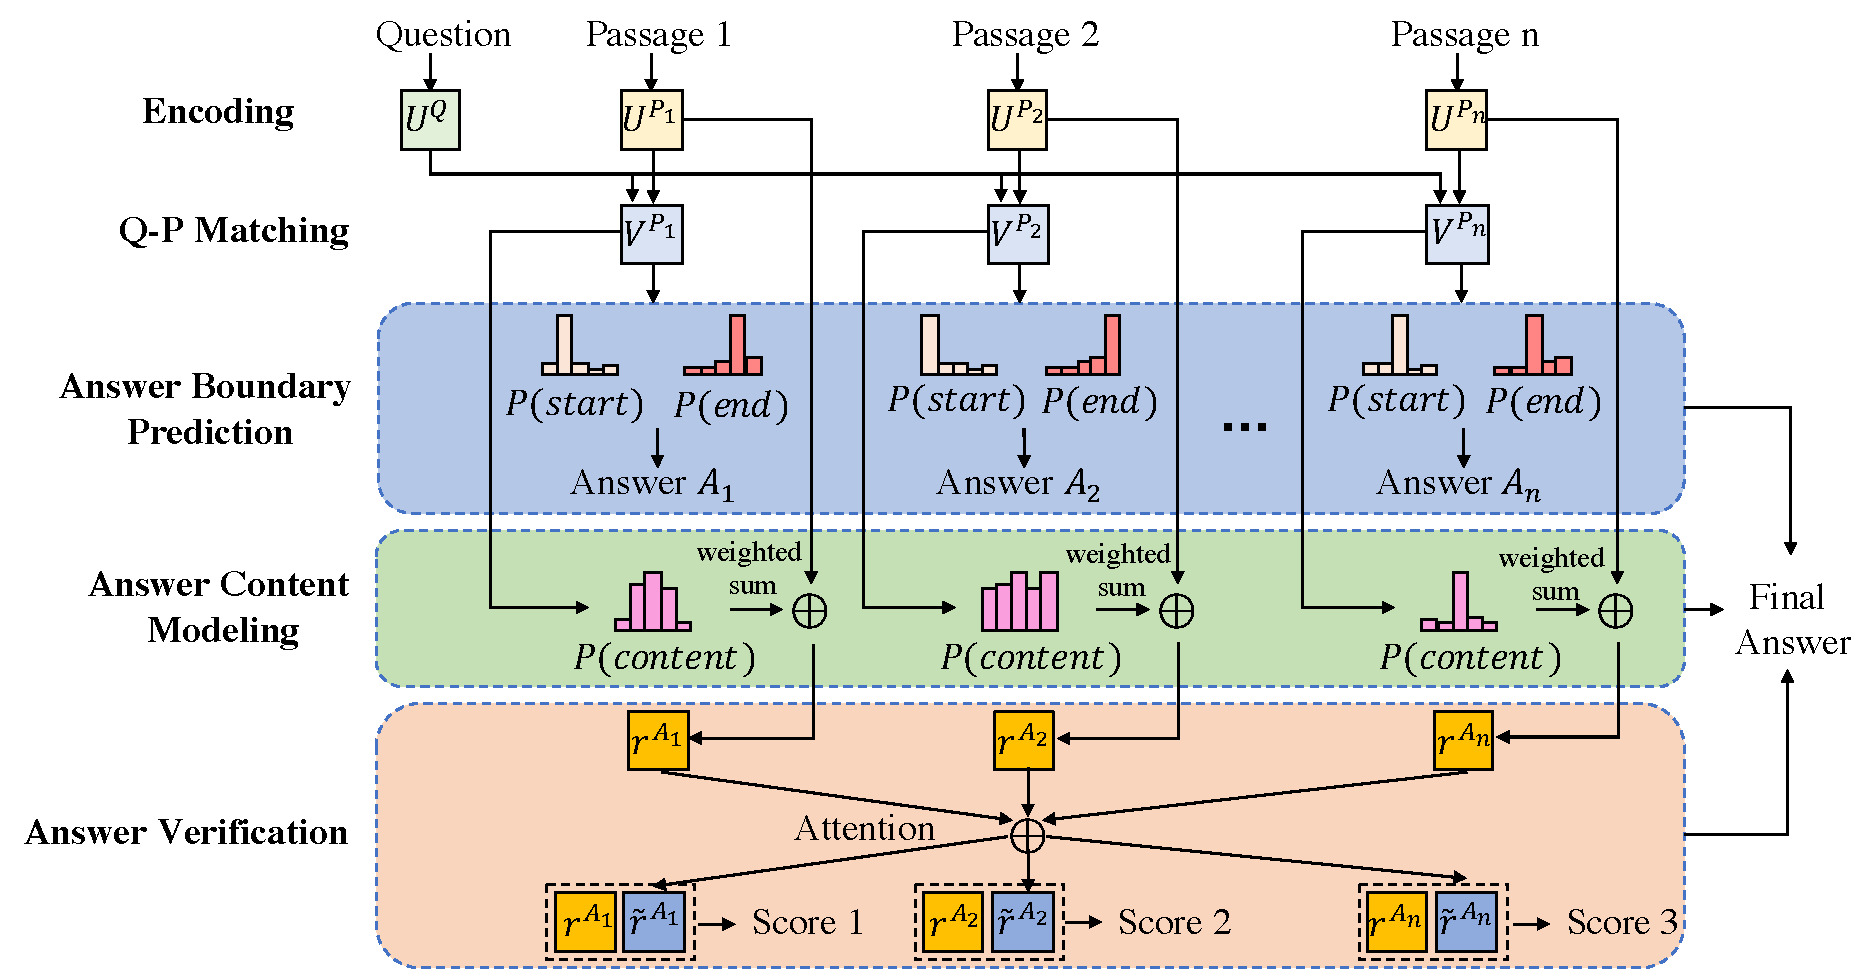
\includegraphics[width=0.85\textwidth]{architecture}
\caption{The overall architecture of our proposed network. The network
contains layers of symmetric convolution (encoder) and deconvolution (decoder).
Skip shortcuts are connected every a few (in our experiments, two) layers from
convolutional feature maps to their mirrored deconvolutional feature maps.
The response from a convolutional layer is directly propagated to the corresponding
mirrored deconvolutional layer, both forwardly and backwardly.}
\label{fig1}
\end{figure*}

\section{Very deep convolutional auto-encoder for image restoration}
\label{sec:main}

The proposed framework mainly contains a chain of convolutional layers and symmetric
deconvolutional layers, as shown in Figure \ref{fig1}. Skip connections are connected
symmetrically from convolutional layers to deconvolutional layers. We term our method
``RED-Net''---very deep Residual Encoder-Decoder Networks.


\subsection{Architecture}

The framework is fully convolutional (and deconvolutional.  Deconvolution is essentially unsampling convolution). Rectification layers are added
after each convolution and deconvolution. For low-level image restoration problems, we
use neither pooling nor unpooling in the network as usually pooling discards useful image
details that are essential for these tasks. It is worth mentioning that since the convolutional
and deconvolutional layers are symmetric, the network is essentially pixel-wise prediction,
thus the size of input image can be arbitrary. The input and output of the network are images
of the same size $w\times h\times c$, where $w$, $h$ and $c$ are width, height and number of channels.

Our main idea is that the convolutional layers act as a feature extractor, which preserve the
primary components of objects in the image and meanwhile eliminating the corruptions.
After forwarding through the convolutional layers, the corrupted input  image is converted into
a ``clean" one. The subtle details of the image contents may be lost during this process.
The deconvolutional layers are then combined to recover the details of image contents.
The output of the deconvolutional layers is the recovered clean version of the input image.
Moreover, we add skip connections  from a convolutional layer to its corresponding
mirrored deconvolutional layer. The passed convolutional feature maps are summed to the
deconvolutional feature maps element-wise, and passed to the next layer after rectification.
Deriving from the above architecture, we have used two networksvin our experiments, which are of 20 layers
 and 30 layers
respectively, for image denoising, image super-resolution, JPEG deblocking and image inpainting.



\subsection{Deconvolution decoder}

Architectures combining layers of convolution and deconvolution~\cite{DBLP:conf/iccv/NohHH15,
hong2015decoupled} have been proposed for semantic segmentation recently. In contrast to
convolutional layers, in which multiple input activations within a filter window are fused
to output a single activation, deconvolutional layers associate a single input activation with
multiple outputs. Deconvolution is usually used as {\em learnable up-sampling layers}.

 In our network,
the convolutional layers successively down-sample the input image content into a  small
size abstraction. Deconvolutional layers then up-sample the abstraction back into its original resolution.

Besides the use of skip connections, a main difference between our model and
~\cite{DBLP:conf/iccv/NohHH15,hong2015decoupled} is that our network is fully convolutional and
deconvolutional, i.e., without pooling and un-pooling. The reason is that for low-level image restoration,
the aim is to eliminate low level corruption while preserving image details instead of learning
image abstractions. Different from high-level applications such as segmentation or recognition,
pooling typically eliminates the abundant image details and can deteriorate restoration performance.



One can simply replace deconvolution with convolution, which results in an architecture that is
very similar to recently proposed very deep fully convolutional neural networks
~\cite{DBLP:conf/cvpr/LongSD15,DBLP:journals/pami/DongLHT16}. However, there exist essential
differences between a fully convolution model and our model. Take image denoising as an example.
We compare the 5-layer and 10-layer fully convolutional network with our network
(combining convolution and deconvolution, but without skip connection). For fully convolutional
networks, we use padding or up-sampling the input to make the input and output be of the same size.
For our network, the first 5 layers are convolutional and the second 5 layers are deconvolutional.
All the other parameters for training are identical, i.e., trained with SGD and learning rate of
$10^{-6}$, noise level $\sigma=70$. The Peak Signal-to-Noise Ratio (PSNR) on the validation set
is reported, which shows that using deconvolution works better than the fully convolutional
counterpart, as shown in Figure \ref{fig2}.


Furthermore, in Figure \ref{fig3}, we visualize some results that are outputs of layer 2, 5, 8 and 10
from the 10-layer fully convolutional network and ours. In the fully convolution case, the noise
is eliminated step by step, i.e., the noise level is reduced after each layer. During this process,
the details of the image content may be lost. Nevertheless, in our network, convolution  preserves
the primary image content. Then deconvolution is used to compensate the details.


\begin{figure}[htb!]
\centering
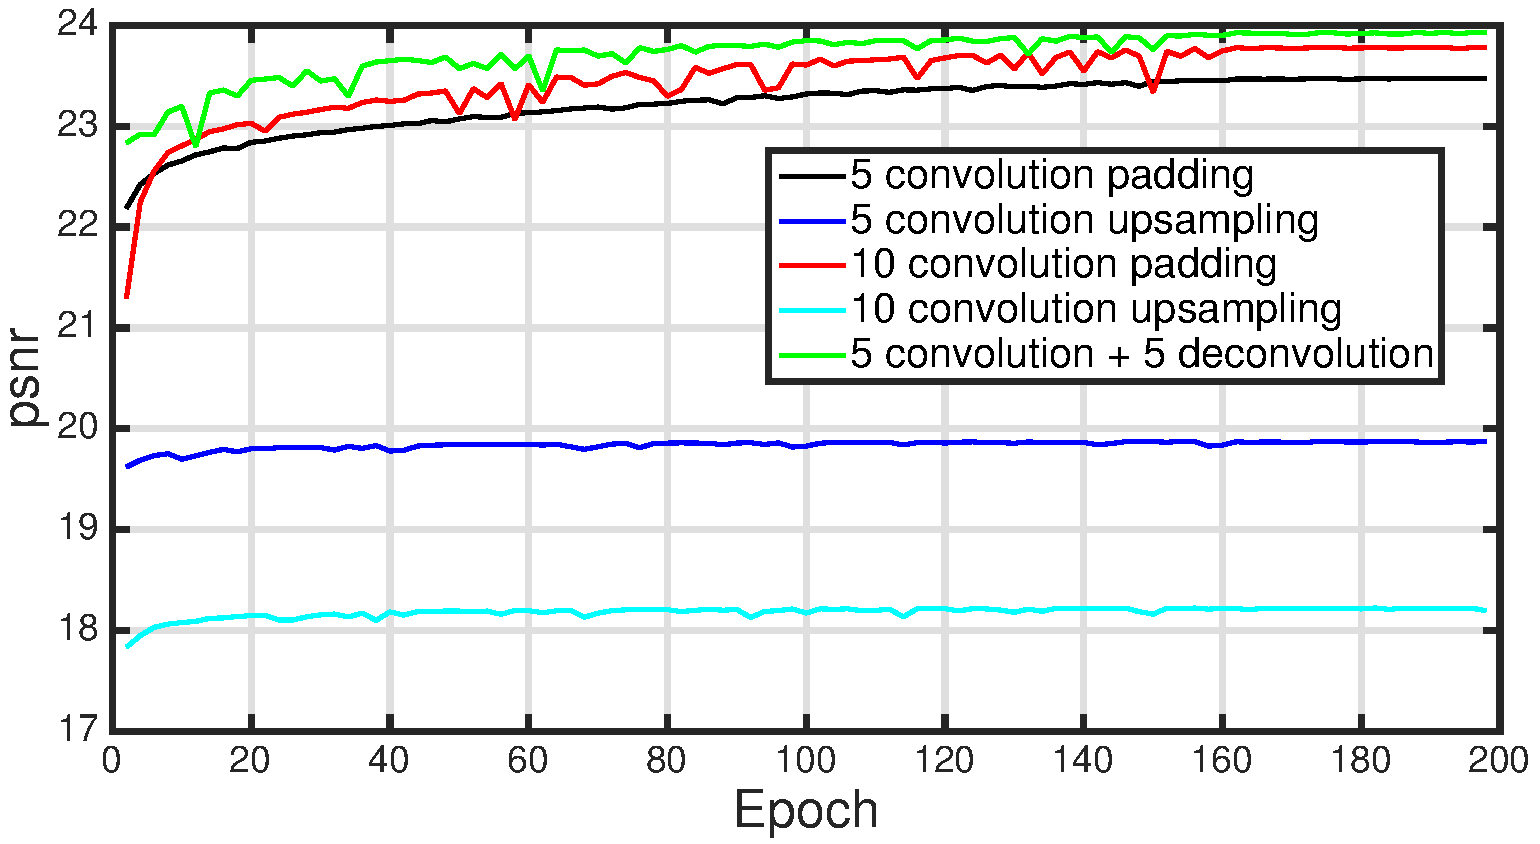
\includegraphics[width=0.48\textwidth]{conv-vs-decv}
\caption{ PSNR  values  on the validation set during training. Our model  exhibits better PSNR
than the compared ones upon convergence.}
\label{fig2}
\end{figure}



\begin{figure}[htb!]
\centering
\subfigure[]{ 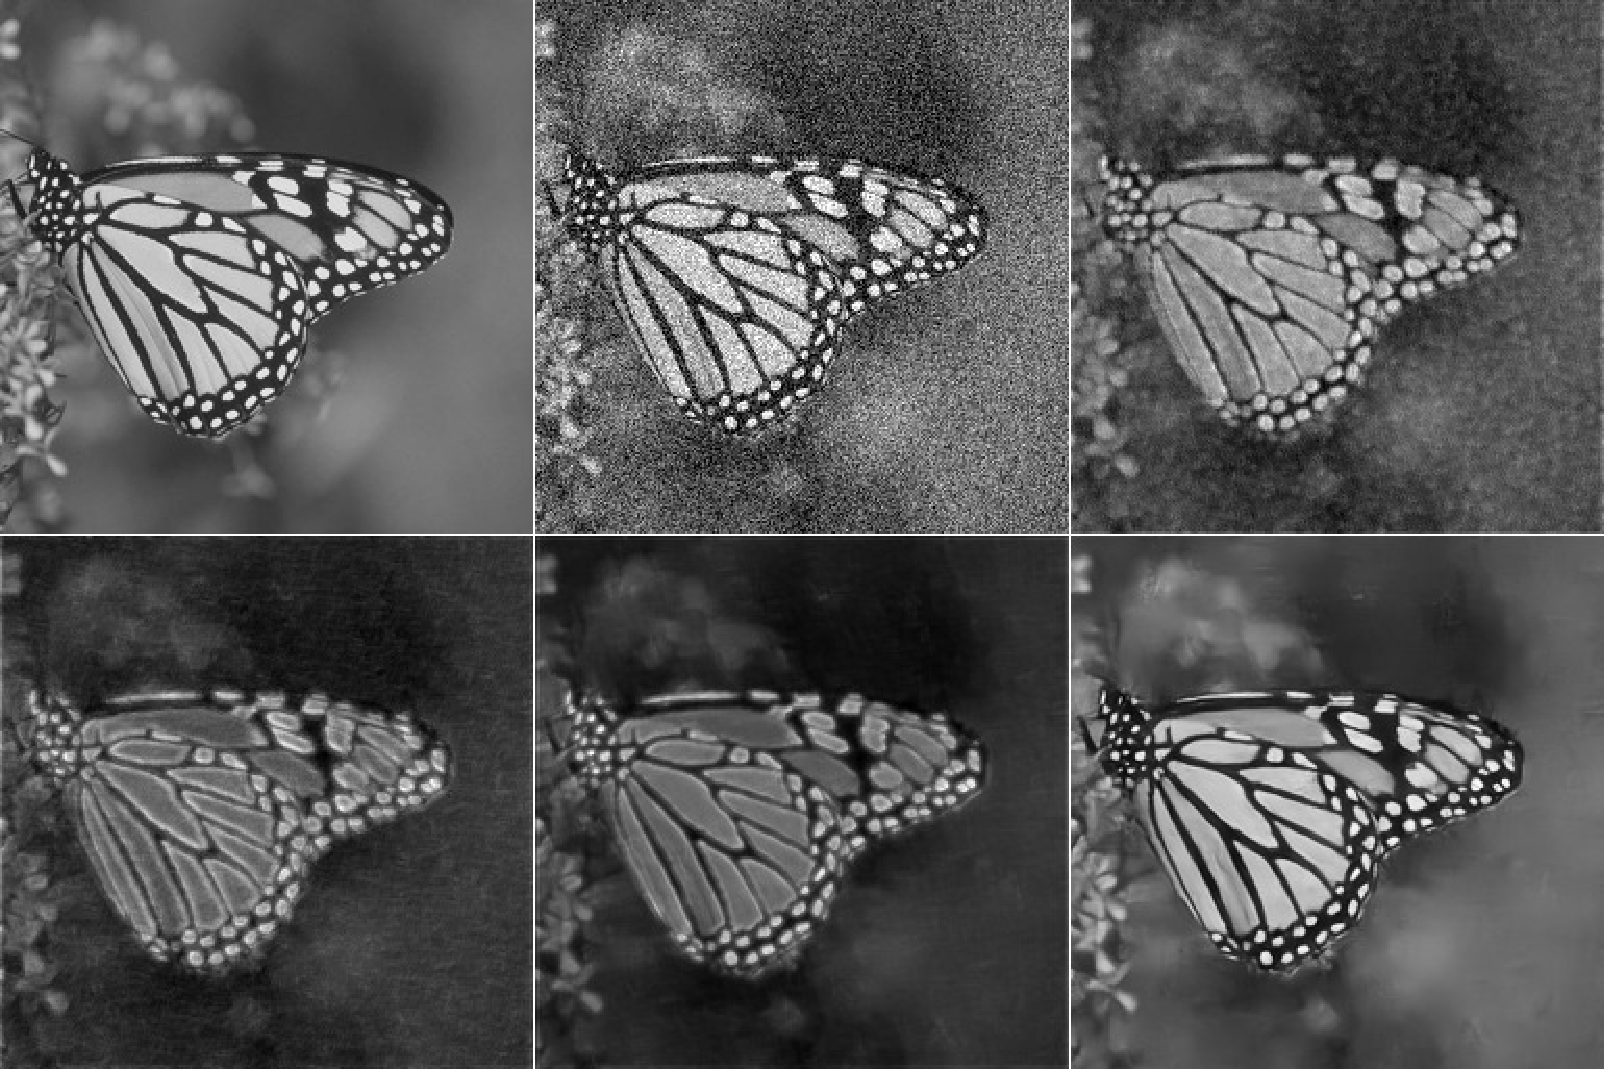
\includegraphics[width=0.48\textwidth]{show-denoising-conv} }
\subfigure[]{ 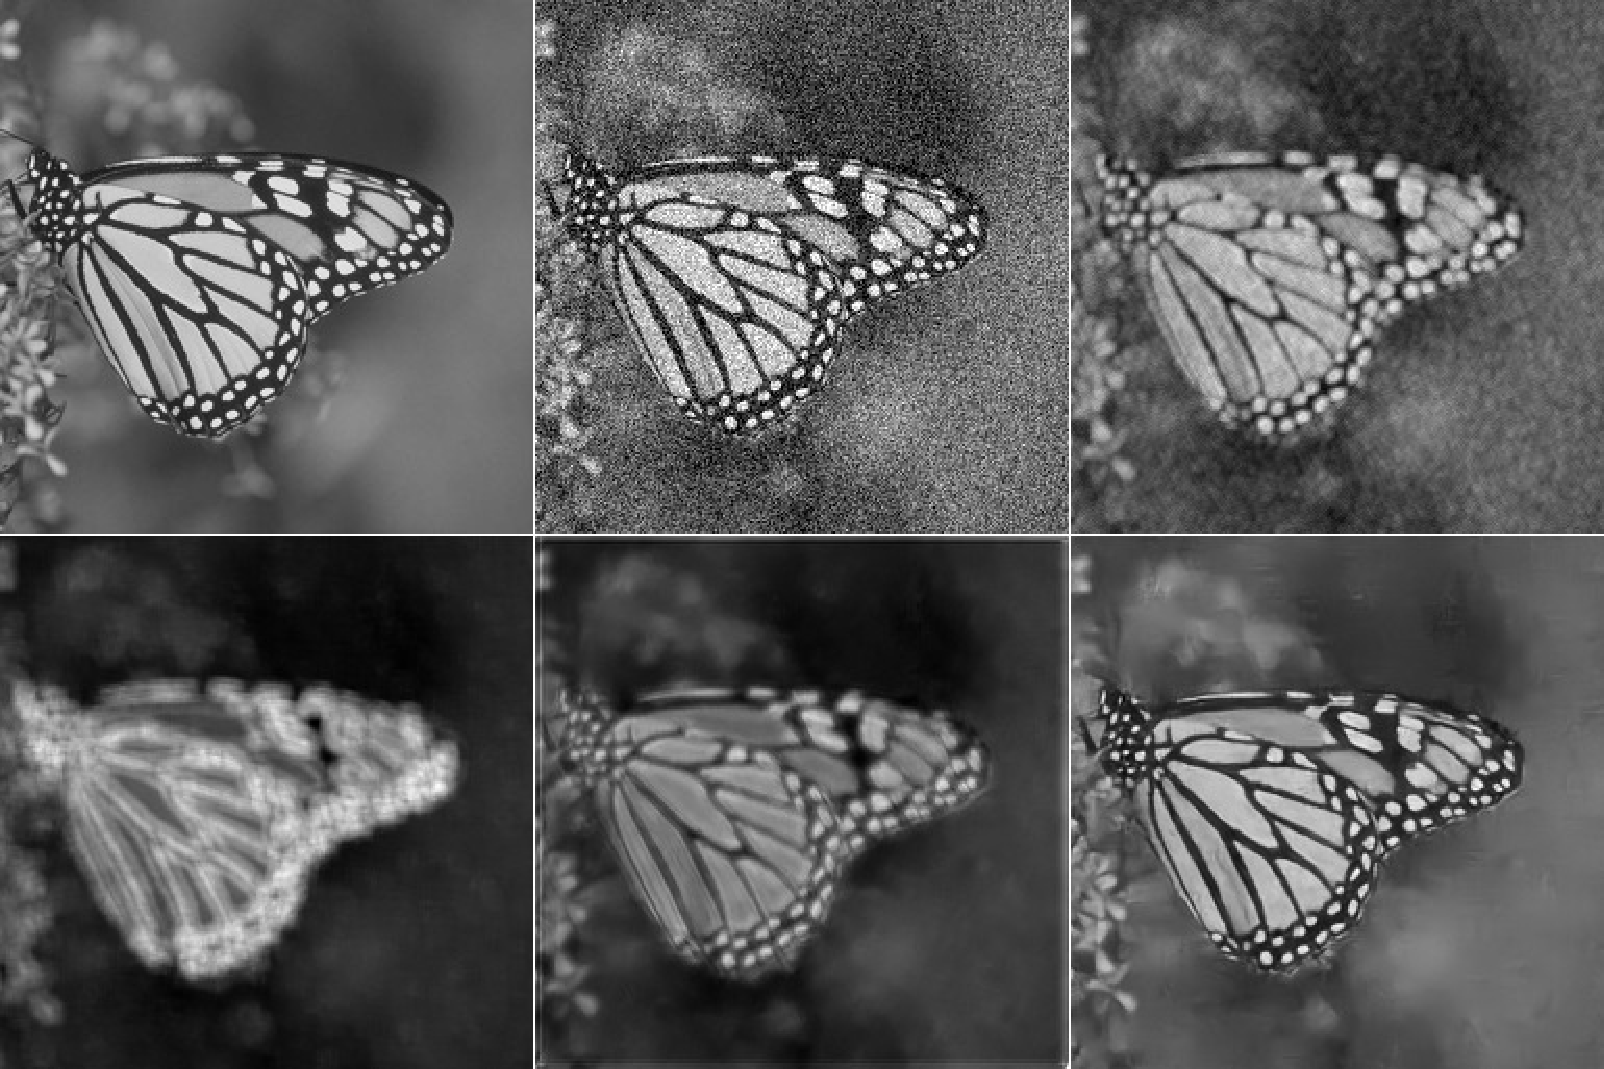
\includegraphics[width=0.48\textwidth]{show-denoising-decv} }
\caption{ (a) Visualization of the 10-layer fully convolutional network. The images from
top-left to bottom-right are: clean image, noisy image, output of conv-2, output of conv-5,
output of conv-8 and output of conv-10, where ``conv-$i$" stands for the $i$-th convolutional layer;
(b) Visualization of the 10-layer convolutional and deconvolutional network. The images from
top-left to bottom-right are: clean image, noisy image, output of conv-2, output of conv-5,
output of deconv-3 and output of deconv-5, where ``deconv-$i$" stands for the $i$-th deconvolutional layer.}
\label{fig3}
\end{figure}




\subsection{Skip connections}

An intuitive question is that, is a network with deconvolution able to recover image details from
the image abstraction only? We find that in shallow networks with only a few layers
of convolution layers, deconvolution is able to recover the details. However, when the
network goes deeper or using operations such as max pooling, even with deconvolution layers, it does not work
that well, possibly because too much details are already lost in the convolution and pooling.


The second question is that, when our network goes deeper, does it achieve performance gain?
We observe that deeper networks in image restoration tasks tend to easily suffer from
performance degradation. The reason may be two folds. First of all, with more layers of
convolution, a significant amount of image details could be lost or corrupted. Given only the image abstraction,
recovering its details is an under-determined problem. Secondly, in terms of optimization,
deep networks often suffer from gradients vanishing and become much harder to train---a problem
that is well addressed in the literature of neural networks.


To address the above two problems, inspired by highway networks \cite{DBLP:journals/corr/SrivastavaGS15}
and deep residual networks \cite{DBLP:journals/corr/HeZRS15}, we add skip connections between
two corresponding convolutional and deconvolutional layers as shown in Figure \ref{fig1}.
A building block is shown in Figure \ref{fig4}. There are two reasons for using such connections.
First, when the network goes deeper, as mentioned above, image details can be lost, making deconvolution
weaker in recovering them. However, the feature maps passed by skip connections carry much image detail,
which helps deconvolution to recover an improved clean version of the image. Second, the skip connections also achieve
benefits on back-propagating the gradient to bottom layers, which makes training deeper network much
easier as observed in \cite{DBLP:journals/corr/SrivastavaGS15} and \cite{DBLP:journals/corr/HeZRS15}.

Note that our skip layer connections are very different from the ones proposed in
\cite{DBLP:journals/corr/SrivastavaGS15} and \cite{DBLP:journals/corr/HeZRS15}, where the only concern
is on the optimization side. In our case, we want to pass information of the convolutional feature maps
to the corresponding deconvolutional layers. The very deep highway networks
\cite{DBLP:journals/corr/SrivastavaGS15} are essentially feedforward long short-term memory (LSTMs)
with forget gates, and the CNN layers of deep residual network \cite{DBLP:journals/corr/HeZRS15}
are feedforward LSTMs without gates. Note that our networks are in general not in the format of
standard feedforward LSTMs.

\begin{figure}[htb!]
\centering
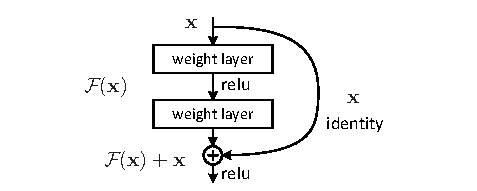
\includegraphics[width=0.48\textwidth]{block}
\caption{An example of a building block in the proposed framework. The rectangle in solid and
dotted lines denote convolution and deconvolution respectively. $\oplus$ denotes element-wise sum of feature maps.}
\label{fig4}
\end{figure}

Instead of directly learning the mappings from the input $X$ to the output $Y$, we would like the network
to fit the residual~\cite{DBLP:journals/corr/HeZRS15} of the problem, which is denoted as $\mathcal{F}(X)=Y-X$.
Such a learning strategy is applied to inner blocks of the encoding-decoding network to make training more
effective. Skip connections are passed every two convolutional layers to their mirrored deconvolutional
layers. Other configurations are possible and our experiments show that this configuration already works
very well. Using such shortcuts makes the network easier to be trained and gains restoration performance
by increasing the network depth.




\subsection{Training}

In general, there are three types of layers in our network: convolution, deconvolution
and element-wise sum. Each layer is followed by a Rectified Linear Unit (ReLU)
~\cite{DBLP:conf/icml/NairH10}. Let $X$ be the input, the convolutional and
deconvolutional layers are expressed as:
\begin{equation}
F(X) = \max(0,W_k * X + B_k),
\end{equation}
where $W_k$ and $B_k$ represent the filters and biases, and $*$ denotes either
convolution or deconvolution operation for the convenience of formulation.
For element-wise sum layer, the output is the element-wise sum of two inputs
of the same size, followed by the ReLU activation:
\begin{equation}
F(X_1,X_2) = \max(0, X_1 + X_2)
\end{equation}

Learning the end-to-end mapping from corrupted images to clean images needs to
estimate the weights $\Theta$ represented by the convolutional and deconvolutional
kernels. Specifically, given a collection of $N$ training sample pairs $\{X^i,Y^i\}$,
where $X^i$ is a noisy image and $Y^i$ is the clean version as the groundtruth.
We minimize the following Mean Squared Error (MSE):
\begin{equation}
  \mathcal{L}(\Theta) = \frac{1}{N}\sum_{i=1}^{N}\|\mathcal{F}(X^i;\Theta)-Y^i\|_F^2.
\label{eq1}
\end{equation}

Traditionally, a  network can learn the mapping from the corrupted image to the clean version
directly. However, our network learns for the additive corruption from the input since there
is a skip connection between the input and the output of the network.
%
%
%
We found that optimizing for the corruption converges better than
optimizing for the clean image. In the extreme case, if the input is a clean image, it would be easier
to push the network to be zero mapping (learning the corruption) than to fit an identity
mapping (learning the clean image) with a stack of nonlinear layers.

We implement and train our network using Caffe~\cite{jia2014caffe}. Empirically, we find
that using Adam~\cite{DBLP:journals/corr/KingmaB14} with base learning rate of $10^{-4}$ for
training converges faster than traditional stochastic gradient descent (SGD). The base
learning rate for all layers are the same, different from ~\cite{DBLP:journals/pami/DongLHT16,
DBLP:conf/nips/JainS08}, in which a smaller learning rate is set for the last layer.
This  is not necessary in our network. Specifically, gradients with respect to the
parameters of $i$th layer is firstly computed as:
\begin{equation}
g = \nabla_{\theta_i}\mathcal{L}(\theta_i).
\end{equation}
Then, the two momentum vectors are computed as:
\begin{equation}
m = \beta_1m + (1 - \beta_1)g,\quad v = \beta_2v + (1-\beta_2)g^2.
\end{equation}
The update rule is:
\begin{equation}
\alpha = \alpha\sqrt{1-\beta_2^t}/(1-\beta_1^t), \quad \theta_i=\theta_i-\alpha m/(\sqrt{v}+\epsilon).
\end{equation}
$\beta_1$, $\beta_2$ and $\epsilon$ are set as the recommended values in~\cite{DBLP:journals/corr/KingmaB14}.

300 images from the Berkeley Segmentation Dataset (BSD)~\cite{MartinFTM01} are used to
generate image patches as the training set for each image restoration task.
%
%
%




\subsection{Testing}

Although trained on local patches, our network can perform restoration on images of arbitrary sizes.
Given a testing image, one can simply go forward through the network, which is already able to
 outperform existing methods. To achieve even better results, we propose
to process a corrupted image on multiple orientations. Different from segmentation, the
filter kernels in our network only eliminate the corruptions, which is usually not sensitive
to the orientation of image contents in low level restoration tasks. Therefore, we can rotate
and mirror flip the kernels and perform forward multiple times, and then average the output to
achieve an ensemble of multiple tests. We see that this can lead to slightly better performance.


%\section{Extensions}
%\label{sec:extensions}
%\label{sec:extension}
Inherently, there is no unique "ground-truth" image that conforms to the given semantic layout. For example, given a semantic layout of a car, we can synthesize a black, red, or white car and it might be facing front or back. Our CRN is able to generate diverse images explicitly.

In order to generate $k$ images from our network, we simply change the number of feature channels in the final layer from $3$ to $3k$. Every three feature maps can form an image, totally $k$ images. With $k$ output images, we also need to adjust our loss function. We need a loss function that measures the distance between a reference image in the training data and $k$ generated images. Intuitively, we should not penalize as long as the reference is close to one of $k$ output images. Let $g_u(L,\theta)$ denote the $u$-th image the network synthesize. The loss $\lL(I,L;\theta)$ for our CRN with $k$ output images would become \cite{Lee2016},

\begin{equation}
\min_u{\sum_l{\lambda_l\| \Phi_l(I)-\Phi_l(g_u(L;\theta))\|_1}}.
\label{eqn:diversity_loss_1}
\end{equation}
This loss encourage diversity in the output images, because having the same output images does not help reduce the loss. We only need one of them for comparison. This loss is similar to k-means clustering loss and the centroid is unlikely to collide.

Furthermore, the loss (\ref{eqn:diversity_loss_1}) can be improved as we could construct up to $k^c$ different images from just $k$ output images: for each class out of $c$ semantic classes, we can choose one $k$ images to fill the content of the regions of that class. However, it is computationally intractable to explicit compute $k^c$ images.

In fact, computing the loss between the reference image and $k^c$ constructed images can be computed efficiently, semantic classes are sperable during construction. Intuitively, as long as one of $k$ images has similar output with the reference image in the areas of that semantic class, we should not penalize. Therefore, we can have a loss that sum up the per-class losses:
$$
\sum_{p=1}^c{\min_u{\sum_l{\lambda_l\|mask(L,p,l) \odot \left(\Phi_l(I)-\Phi_l(g_u(L;\theta))\right)\|_1}}},
$$
where $mask(L,p,l)$ is a mask image $M$ with the same shape of $\Phi_l$. Suppose $M$ has shape $m'\times n' \times w'$ and let $L'$ be the resized semantic layout of $L$ with size $m'\times n'\times c$. Then $M_{i,j,z}=L'_{i,j,p}$ for all $z$. $M$ eliminates penalty in regions where the semantic class is not $p$.

\begin{figure}[H]
  \centering
  \begin{tabular}{@{}c@{\hspace{0.5mm}}c@{}}
  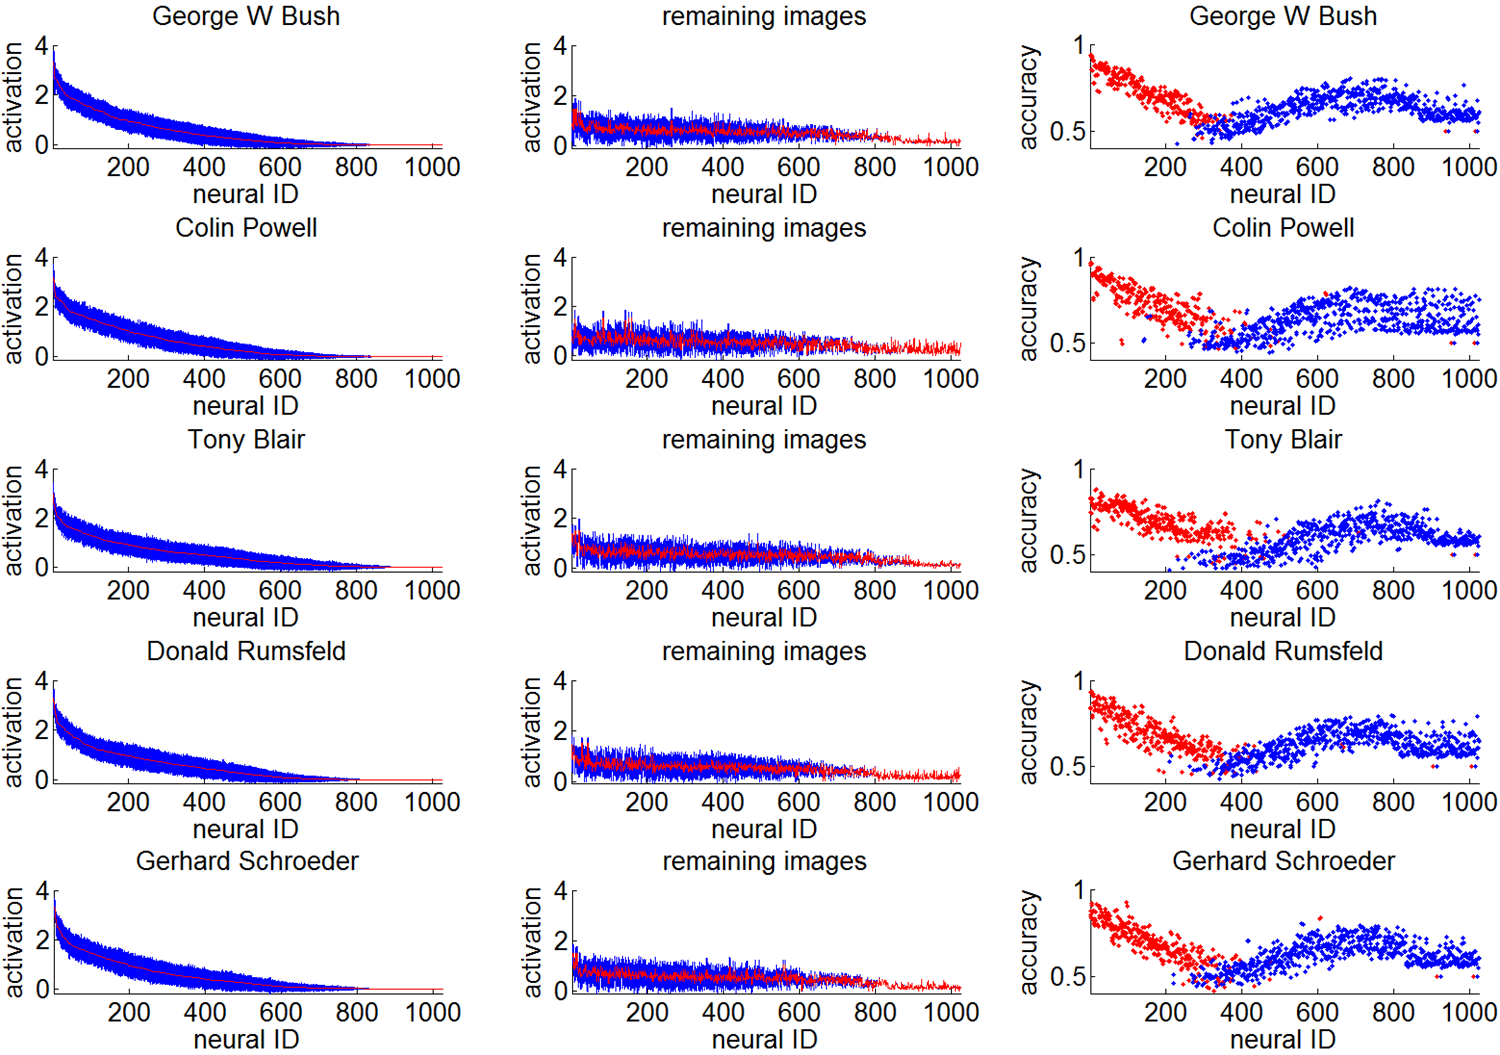
\includegraphics[width=0.235\textwidth]{figures/diversity/1.png}&
  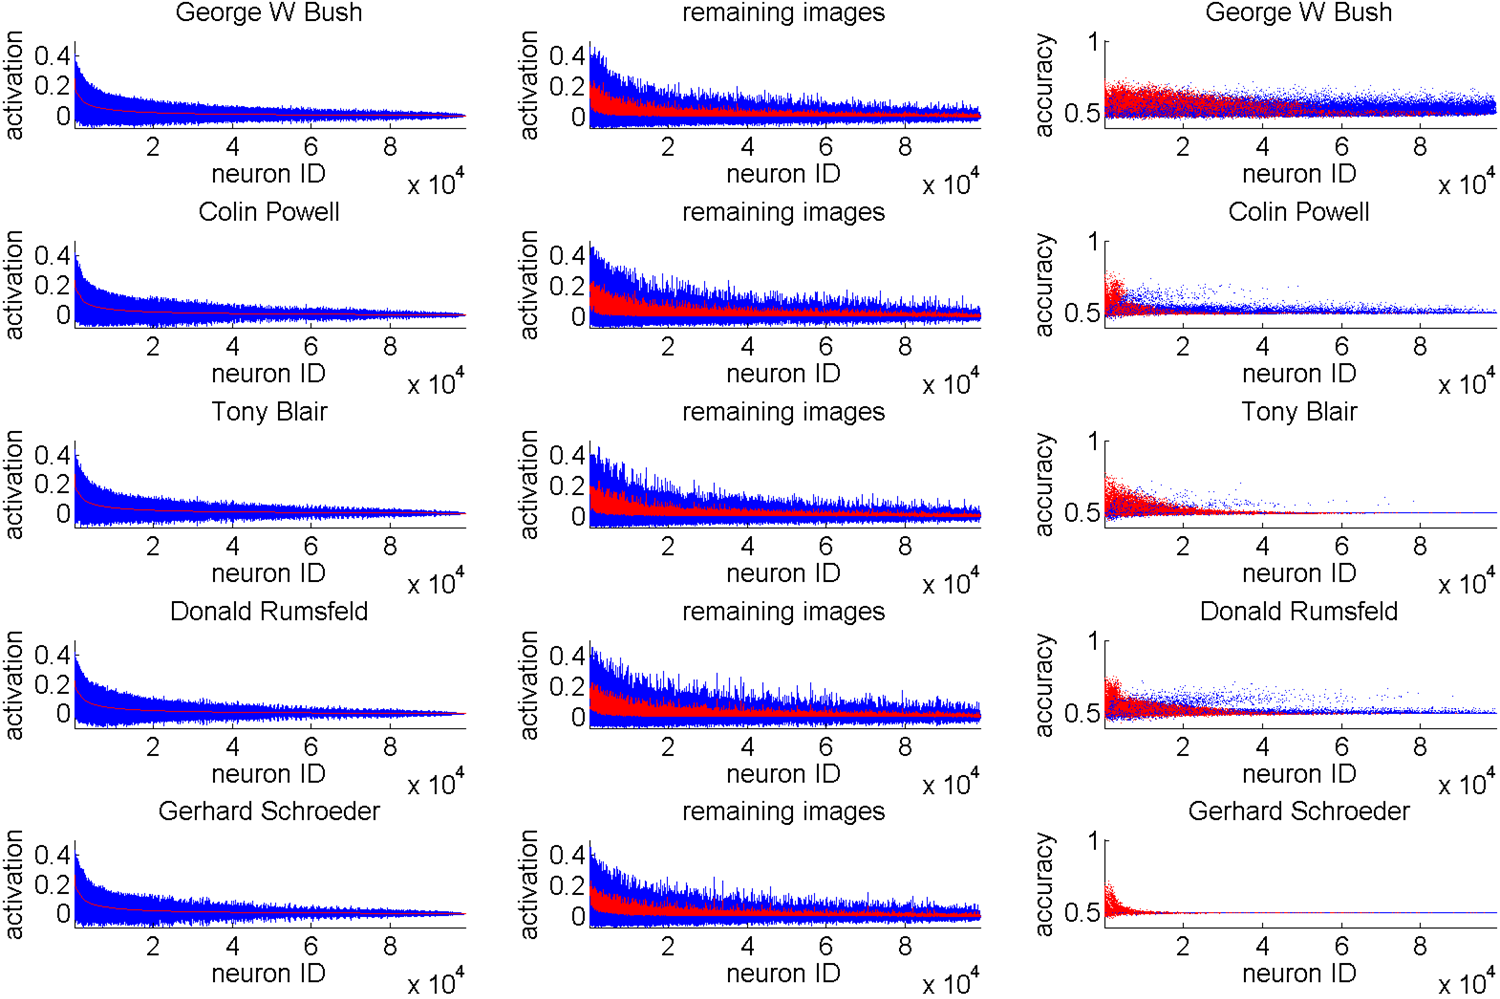
\includegraphics[width=0.235\textwidth]{figures/diversity/2.png}\\
  Output A& Output B\\
  \end{tabular}
  \caption{diversity.}
\label{fig:diversity}
\end{figure}


\section{Baselines}
\label{sec:baselines}
%\vspace{\sectionReduceTop}
\section{VQA Baselines and Methods}
%\vspace{\sectionReduceBot}
\begin{figure*}[h]
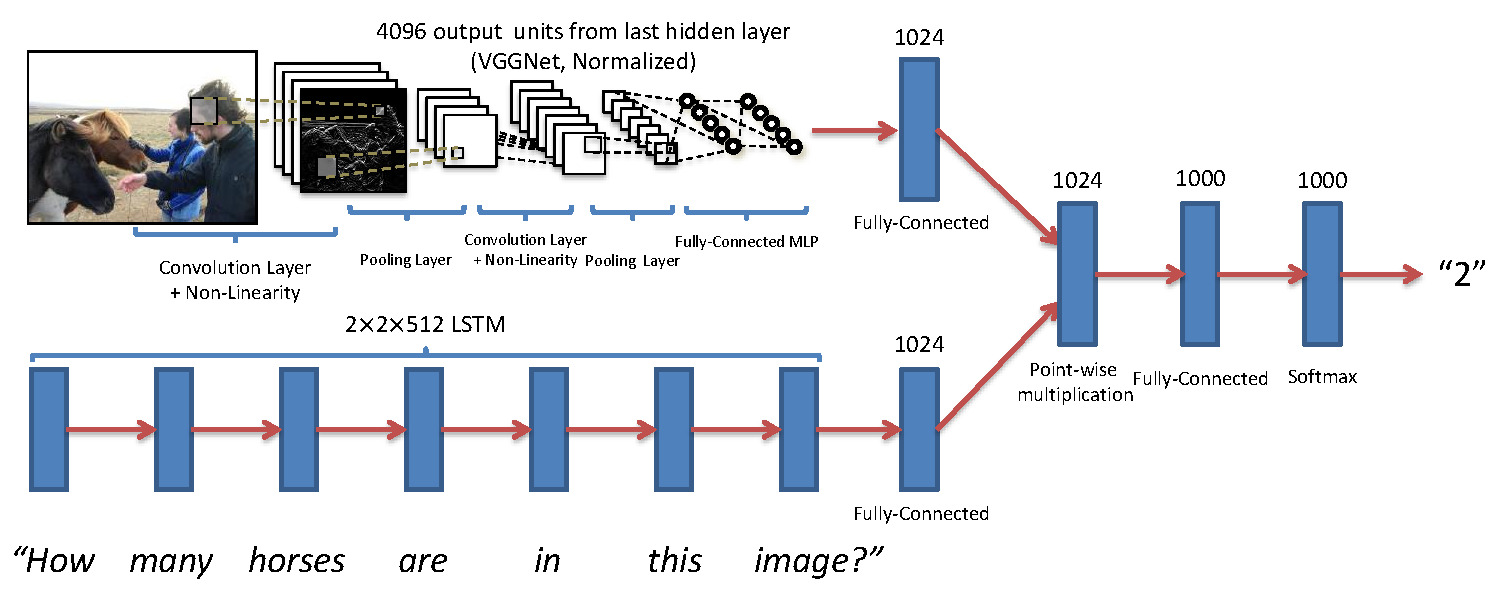
\includegraphics[width=1\linewidth]{figures/best_model_compressed.pdf}
\centering
\caption{Our best performing model (deeper LSTM Q + norm I). This model uses a two layer LSTM to encode the questions and the last hidden layer of VGGNet~\cite{Simonyan14c} to encode the images. The image features are then $\ell_2$ normalized. Both the question and image features are transformed to a common space and fused via element-wise multiplication, which is then passed through a fully connected layer followed by a softmax layer to obtain a distribution over answers.}
\label{fig:best_model}
%\vspace{\captionReduceBot}
\end{figure*}
In this section, we explore the difficulty of the VQA dataset for the MS COCO images using several baselines 
and novel methods. We train on VQA train+val. Unless stated otherwise, all human accuracies are on test-standard, machine accuracies are on test-dev, and results involving human captions (in gray font) are trained on train and tested on val (because captions are not available for test). 

\subsection{Baselines}
\label{sec:baselinesmain}
We implemented the following baselines:
\begin{enumerate}
\item \textbf{random:} We randomly choose an answer from the top 1K answers of the VQA train/val dataset.

\item \textbf{prior (``yes''):} We always select the most popular answer (``yes'') for both the open-ended and multiple-choice tasks. Note that ``yes'' is always one of the choices for the multiple-choice questions.

\item \textbf{per Q-type prior:} For the open-ended task, we pick the most popular answer per question type (see the appendix for details). For the multiple-choice task, we pick the answer (from the provided choices) that is most similar to the picked answer for the open-ended task using cosine similarity in Word2Vec\cite{word2vec} feature space.

\item \textbf{nearest neighbor:} Given a test image, question pair, we first find the $K$ nearest neighbor questions and associated images from the training set. See appendix for details on how neighbors are found. Next, for the open-ended task, we pick the most frequent ground truth answer from this set of nearest neighbor question, image pairs. Similar to the ``per Q-type prior'' baseline, for the multiple-choice task, we pick the answer (from the provided choices) that is most similar to the picked answer for the open-ended task using cosine similarity in \\ Word2Vec\cite{word2vec} feature space.
\end{enumerate}

%If we randomly choose an answer from the top 1K answers of the VQA train/val dataset, 
%the test-standard accuracy is $0.12\%$. 
%If we always select the most popular answer (``yes''), the accuracy is $29.72\%$. Picking the most popular answer per question type does $37.55\%$ and a nearest neighbor approach does $42.73\%$ on test-standard (see the appendix for details).
%For testing, we use the same train/val/test splits as COCO$^2$. 
%we split our real image dataset into a training and testing dataset. Our training dataset contains $30,000$ images and our testing dataset contains $20,000$ images. \jiasen{change image numbers, also including the NN baseline?}
\vspace{-5pt}
\subsection{Methods}
\label{sec:methods}
For our methods, we develop a 2-channel vision (image) + language (question) model that culminates with a softmax over $K$ possible outputs. We choose the top $K = 1000$ most frequent answers as possible outputs. This set of answers covers $82.67\%$ of the train+val answers. We describe the different components of our model below:

\textbf{Image Channel:} This channel provides an embedding for the image. We experiment with two embeddings -- 
\begin{compactenum}
\item \textbf{I:} The activations from the last hidden layer of VGGNet~\cite{Simonyan14c} are used as 4096-dim image embedding.
\item \textbf{norm I:} These are $\ell_2$ normalized activations from the last hidden layer of VGGNet~\cite{Simonyan14c}.
\end{compactenum}

\textbf{Question Channel:} This channel provides an embedding for the question. We experiment with three embeddings --
\begin{compactenum}
\item \textbf{Bag-of-Words Question (BoW Q)}: The top 1,000 words in the questions are used to create a bag-of-words representation. Since there is a strong correlation between the words that start a question and the answer (see \figref{fig:AnsPerQues}), we find the top 10 first, second, and third words of the questions and create a 30 dimensional bag-of-words representation. These features are concatenated to get a 1,030-dim embedding for the question.
\item \textbf{LSTM Q:} An LSTM with one hidden layer is used to obtain 1024-dim embedding for the question. The embedding obtained from the LSTM is a concatenation of last cell state and last hidden state representations (each being 512-dim) from the hidden layer of the LSTM. Each question word is encoded with 300-dim embedding by a fully-connected layer + tanh non-linearity which is then fed to the LSTM. The input vocabulary to the embedding layer consists of all the question words seen in the training dataset.
\item \textbf{deeper LSTM Q:} An LSTM with two hidden layers is used to obtain 2048-dim embedding for the question. The embedding obtained from the LSTM is a concatenation of last cell state and last hidden state representations (each being 512-dim) from each of the two hidden layers of the LSTM. Hence 2 (hidden layers) x 2 (cell state and hidden state) x 512 (dimensionality of each of the cell states, as well as hidden states) in \figref{fig:best_model}. This is followed by a fully-connected layer + tanh non-linearity to transform 2048-dim embedding to 1024-dim. The question words are encoded in the same way as in LSTM Q.   
\end{compactenum}

\textbf{Multi-Layer Perceptron (MLP):} The image and question embeddings 
%obtained from the image and question channels respectively 
are combined to obtain a single embedding. 
\begin{compactenum}
\item For \textbf{BoW Q + I} method, we simply concatenate the BoW Q and I embeddings. 
\item For \textbf{LSTM Q + I}, and \textbf{deeper LSTM Q + norm I} (\figref{fig:best_model}) methods, the image embedding is first transformed to 1024-dim by a fully-connected layer + tanh non-linearity to match the LSTM embedding of the question. The transformed image and LSTM embeddings (being in a common space) are then fused via element-wise multiplication. 
\end{compactenum}
This combined image + question embedding is then passed to an MLP -- a fully connected neural network classifier with 2 hidden layers and 1000 hidden units (dropout 0.5) in each layer with tanh non-linearity, followed by a softmax layer to obtain a distribution over $K$ answers. The entire model is learned end-to-end with a cross-entropy loss. VGGNet parameters are frozen to those learned for ImageNet classification and not fine-tuned in the image channel.   

We also experimented with providing captions as input to our model. Similar to \tableref{table:commonsense_acc}, we assume that a human-generated caption is given as input. We use a bag-of-words representation containing the 1,000 most popular words in the captions as the caption embedding (\textbf{Caption}). For \textbf{BoW Question + Caption (BoW Q + C)} method, we simply concatenate the BoW Q and C embeddings. 
%\jiasen{We don't know the coverage on test set, should we report the coverage on train+val set?} All baselines train a softmax neural network classifier with a single hidden layer containing 50 units. \jiasen{We have MLP baseline and LSTM baseline. For the MLP baseline, we train a softmax neural network classifier with 2 hidden layer each containing 1000 units. We use Tanh() as non-linear function and apply Dropout with probability 0.5 in each hidden layer.} 
%We experiment with three models: 
%(i) a multi-layer perceptron (MLP) neural network classifier with 2 hidden layers and 1000 hidden 
%units (dropout 0.5) in each layer with tanh non-linearity,  
%(ii) an LSTM model followed by a softmax layer to obtain a distribution over answers, and
%(iii) a two layer deeper LSTM model followed by softmax layer to obtain a distribution over answers.
%We experimented with five inputs for the MLP model. \textbf{Bag-of-Words Question (BoW Q)}: The top 1,000 words in the questions are used to create a bag-of-words representation. Since there is a strong correlation between the words that start a question and the answer (see \figref{fig:AnsPerQues}), we find the top 10 first, second, and third words of the questions and create a 30 dimensional bag-of-words representation. These features are concatenated to get a 1,030 dimensional input representation. \textbf{Caption:} Similar to \tableref{table:commonsense_acc}, we assume that a human-generated caption is given as input. We use a bag-of-words representation containing the 1,000 most popular words in the captions as the input feature. \textbf{Image (I):} We use the last hidden layer of VGGNet~\cite{Simonyan14c} as our 4096-dim feature. We also report the learned baseline results on \textbf{BoW Question + Image (BoW Q + I)} and \textbf{BoW Question + Caption (BoW Q + C)} by simply concatenating the first hidden layer representations of networks trained on each feature individually. The LSTM model uses a one-hot encoding for the question words, and the same image features as above followed by a linear + tanh transformation to transform the image features to 1024 dimensions to match the LSTM encoding of the question. The question and image encodings are fused via element-wise multiplication. The deeper LSTM Q model uses two hidden layers in the LSTM unlike only one hidden layer in the LSTM model. The deeper LSTM Q + norm I model (\figref{fig:best_model}) has almost the same architecture as the LSTM Q + I model except that it uses deeper LSTM (two hidden layer) and $l2$ normalized image features.

%For LSTM question only baseline, we simply input the question words into the LSTM along and fed into a softmax layer at the last timestep to generate the answers. For the LSTM vis baseline, we use the same VGG Conv Net fc7 layer feature, and use a linear trainsforamtion to map 4096 dimension image feature vectors to 1024 dimensional vector that match the dimension of encoded question feature. We fuse the image and question feature by doing an element-wise multiplication and further fed into a softmax layer. } 
For testing, we report the result on two different tasks: open-ended selects the answer with highest activation from all possible $K$ answers and multiple-choice picks the answer that has the highest activation from the potential answers. 

\subsection{Results}
\label{sec:results}

\begin{table}[t] \scriptsize
\setlength{\tabcolsep}{1.8pt}
\begin{center}
\begin{tabular}{@{} l  c  c  c  c  c  c c c@{}}
%\hline
\toprule
& \multicolumn{4}{c}{Open-Ended} & \multicolumn{4}{c}{ Multiple-Choice} \\

\cmidrule[0.75pt](l){2-5}
\cmidrule[0.75pt](l){6-9}
 & All & Yes/No & Number & Other & All & Yes/No & Number & Other \\
%\hline
\midrule
prior (``yes'') & 29.66 & 70.81 & 00.39 & 01.15 & 29.66 & 70.81 & 00.39 & 01.15 \\
per Q-type prior & 37.54 & 71.03 & 35.77 & 09.38 &  39.45 & 71.02 & 35.86 & 13.34 \\
nearest neighbor & 42.70 & 71.89 & 24.36 & 21.94 & 48.49 & 71.94 & 26.00 & 33.56 \\
BoW Q & \textcolor{black}{48.09} & \textcolor{black}{75.66} &  \textcolor{black}{36.70}& \textcolor{black}{27.14} 
& \textcolor{black}{53.68} & \textcolor{black}{75.71} & \textcolor{black}{37.05} & \textcolor{black}{38.64}\\
I & \textcolor{black}{28.13} & \textcolor{black}{64.01} & 00.42 & \textcolor{black}{03.77}  
&\textcolor{black}{30.53} & \textcolor{black}{69.87} & 00.45 & \textcolor{black}{03.76}\\
BoW Q + I & \textcolor{black}{52.64} & \textcolor{black}{75.55} & 33.67 & \textcolor{black}{37.37} 
& \textcolor{black}{58.97} & \textcolor{black}{75.59} & 34.35 & \textcolor{black}{50.33}\\
LSTM Q & \textcolor{black}{48.76} & \textcolor{black}{78.20} & 35.68 & \textcolor{black}{26.59} 
& \textcolor{black}{54.75} & \textcolor{black}{78.22} & 36.82 &\textcolor{black}{38.78}\\
LSTM Q + I & \textcolor{black}{53.74} & \textcolor{black}{78.94} & 35.24 & \textcolor{black}{36.42} 
& \textcolor{black}{57.17} & \textcolor{black}{78.95}& 35.80 & \textcolor{black}{43.41}\\
deeper LSTM Q & \textcolor{black}{50.39} & \textcolor{black}{78.41} & 34.68 & \textcolor{black}{30.03} 
& \textcolor{black}{55.88} & \textcolor{black}{78.45} & 35.91 &\textcolor{black}{41.13}\\
%\textcolor{red}{deeper LSTM Q} \\
deeper LSTM Q + norm I & \textbf{57.75} & \textbf{80.50} & \textbf{36.77} & \textbf{43.08} 
& \textbf{62.70} & \textbf{80.52}& \textbf{38.22} & \textbf{53.01}\\
%\textcolor{red}{norm I} \\
\midrule
\textcolor{gray}{Caption} & \textcolor{gray}{26.70} & \textcolor{gray}{65.50} & \textcolor{gray}{02.03} & \textcolor{gray}{03.86} 
& \textcolor{gray}{28.29} & \textcolor{gray}{69.79} & \textcolor{gray}{02.06} & \textcolor{gray}{03.82}\\
\textcolor{gray}{BoW Q + C} & \textcolor{gray}{54.70} & \textcolor{gray}{75.82} & \textcolor{gray}{40.12} & \textcolor{gray}{42.56} 
& \textcolor{gray}{59.85} & \textcolor{gray}{75.89} & \textcolor{gray}{41.16}  & \textcolor{gray}{52.53}\\
\bottomrule
\end{tabular}	
\caption{Accuracy of our methods for the open-ended and multiple-choice tasks on the VQA test-dev for real images. 
Q = Question, I = Image, C = Caption. (Caption and BoW Q + C results are on val). 
See text for details.
}
%\vspace{-10pt}
\label{tab:acc}
\end{center}
\end{table}
\tableref{tab:acc} shows the accuracy of our baselines and methods for both the open-ended and multiple-choice tasks on the VQA test-dev for real images.

As expected, the vision-alone model (I) that completely ignores the question performs rather poorly (open-ended: 28.13\% / multiple-choice: 30.53\%). In fact, on open-ended task, the vision-alone model (I) performs worse than the prior (``yes'') baseline, which ignores both the image \emph{and} question (responding to every question with a ``yes''). 

Interestingly, the language-alone methods (per Q-type prior, BoW Q, LSTM Q) that ignore the image perform surprisingly well, with BoW Q achieving 48.09\% on open-ended (53.68\% on multiple-choice) and LSTM Q achieving 48.76\% on open-ended (54.75\% on multiple-choice); both outperforming the nearest neighbor baseline (open-ended: 42.70\%, multiple-choice: 48.49\%). Our quantitative results and analyses suggest that this might be due to the language-model exploiting subtle statistical priors about the question types (e.g. ``What color is the banana?'' can be answered with ``yellow'' without looking at the image). For a detailed discussion of the subtle biases in the questions, please see \cite{yinyang}. 

The accuracy of our \textbf{best model} (deeper LSTM Q + norm I (\figref{fig:best_model}), selected using VQA test-dev accuracies) on VQA test-standard is 58.16\% (open-ended) / 63.09\% (multiple-choice). We can see that our model is able to significantly outperform both the vision-alone and language-alone baselines. As a general trend, results on multiple-choice are better than open-ended. All methods are significantly worse than human performance.
%The accuracy of our \textbf{best model} (deeper LSTM Q + norm I (\figref{fig:best_model}), selected using VQA test-dev accuracies) on VQA test-standard is $\textbf{58.16\%}$.
%The accuracy using only the question is $\sim$48\%, which demonstrates that the type of question is informative of the answer. As expected, results on multiple-choice are better than open-ended. 
%%In comparison to 
%All methods are significantly worse than human performance. 

Our VQA demo is available on CloudCV \cite{cloudcv} -- \url{http://cloudcv.org/vqa}. This will be updated with newer models as we develop them.

%\textcolor{red}{In \tableref{tab:acc}, the results of (Q + I) are very similar to the results of only using the questions, while the addition of captions (Q + C) provides minimal improvement $\sim2-4\%$.} 
To gain further insights into these results, we computed accuracies by question type in \tableref{tab:typeacc}. Interestingly, for question types that require more reasoning, such as ``Is the'' or ``How many'', the scene-level image features do not provide any additional information. However, for questions that can be answered using scene-level information, such as ``What sport,'' 
%or ``What animal''
we do see an improvement. Similarly, for questions whose answer may be contained in a generic caption we see improvement, such as ``What animal''. For all question types, the results are worse than human accuracies.

We also analyzed the accuracies of our best model (deeper LSTM Q + norm I) on a subset of questions with certain specific (ground truth) answers. In \figref{fig:prob_1}, we show the average accuracy of the model on questions with 50 most frequent ground truth answers on the VQA validation set (plot is sorted by accuracy, not frequency). We can see that the model performs well for answers that are common visual objects such as ``wii'', ``tennis'', ``bathroom'' while the performance is somewhat underwhelming for counts (\eg, ``2'', ``1'', ``3''), and particularly poor for higher counts (\eg, ``5'', ``6'', ``10'', ``8'', ``7''). 

In \figref{fig:prob_2}, we show the distribution of 50 most frequently predicted answers when the system is correct on the VQA validation set (plot is sorted by prediction frequency, not accuracy). In this analysis, ``system is correct'' implies that it has VQA accuracy $1.0$ (see section \ref{sec:dataset} for accuracy metric). We can see that the frequent ground truth answers (\eg, ``yes'', ``no'', ``2'', ``white'', ``red'', ``blue'', ``1'', ``green'') are more frequently predicted than others when the model is correct. 

%This observation suggests that the model is probably learning the distribution of answers in the training dataset.

%%%%%%%%%%%%%%%%%%%%%%%%%%%%%%%%%%%%%%%%%%%%%%%%%%%%%%%%%


\begin{table}[h] \scriptsize
\setlength{\tabcolsep}{2pt}
\begin{center}
\begin{tabular}{@{} l  c  c  c  c c c c@{}  }
%\hline
\toprule
& \multicolumn{5}{c}{Open-Ended}   & Human Age & Commonsense\\

%\cline{2-6}
\cmidrule[0.9pt](l){2-6}

\multicolumn{1}{c}{Question} & \multicolumn{3}{c}{K = 1000} & \multicolumn{2}{c}{Human} & To Be Able & To Be Able\\
\cmidrule[0.5pt](lr){2-4}
\cmidrule[0.5pt](l){5-6}

\multicolumn{1}{c}{Type}  & Q & Q + I & Q + C & Q & Q + I & To Answer & To Answer (\%)\\
%\hline
\midrule
what is \textcolor{black}{(13.84)} & \textcolor{black}{23.57} & \textcolor{black}{34.28} & \textcolor{gray}{43.88} & \textcolor{black}{16.86} & \textcolor{black}{73.68} &\textcolor{black}{09.07} & 27.52\\
what color \textcolor{black}{(08.98)} & \textcolor{black}{33.37} & \textcolor{black}{43.53} & \textcolor{gray}{48.61} & \textcolor{black}{28.71} & \textcolor{black}{86.06} &\textcolor{black}{06.60} & 13.22\\
what kind \textcolor{black}{(02.49)} & \textcolor{black}{27.78} & \textcolor{black}{42.72} & \textcolor{gray}{43.88} & \textcolor{black}{19.10} & \textcolor{black}{70.11} &\textcolor{black}{10.55} & 40.34\\
what are \textcolor{black}{(02.32)} & \textcolor{black}{25.47} & \textcolor{black}{39.10} & \textcolor{gray}{47.27} & \textcolor{black}{17.72} & \textcolor{black}{69.49} &\textcolor{black}{09.03} & 28.72\\
what type \textcolor{black}{(01.78)} & \textcolor{black}{27.68} & \textcolor{black}{42.62} & \textcolor{gray}{44.32} & \textcolor{black}{19.53} & \textcolor{black}{70.65} &\textcolor{black}{11.04} & 38.92\\
is the \textcolor{black}{(10.16)} & \textcolor{black}{70.76} & \textcolor{black}{69.87} & \textcolor{gray}{70.50} & \textcolor{black}{65.24} & \textcolor{black}{95.67} &\textcolor{black}{08.51} & 30.30\\
is this \textcolor{black}{(08.26)} & \textcolor{black}{70.34} & \textcolor{black}{70.79} & \textcolor{gray}{71.54} & \textcolor{black}{63.35} & \textcolor{black}{95.43} &\textcolor{black}{10.13} & 45.32\\
how many \textcolor{black}{(10.28)} & \textcolor{black}{43.78} & \textcolor{black}{40.33} & \textcolor{gray}{47.52} & \textcolor{black}{30.45} & \textcolor{black}{86.32} &\textcolor{black}{07.67}& 15.93 \\
are \textcolor{black}{(07.57)} & \textcolor{black}{73.96} & \textcolor{black}{73.58} & \textcolor{gray}{72.43} & \textcolor{black}{67.10} & \textcolor{black}{95.24} &\textcolor{black}{08.65} & 30.63\\
does \textcolor{black}{(02.75)} & \textcolor{black}{76.81} & \textcolor{black}{75.81} & \textcolor{gray}{75.88} & \textcolor{black}{69.96} & \textcolor{black}{95.70} &\textcolor{black}{09.29} & 38.97\\
where \textcolor{black}{(02.90)} & \textcolor{black}{16.21} & \textcolor{black}{23.49} & \textcolor{gray}{29.47} & \textcolor{black}{11.09} & \textcolor{black}{43.56} &\textcolor{black}{09.54} & 36.51\\
is there \textcolor{black}{(03.60)} & \textcolor{black}{86.50} & \textcolor{black}{86.37} & \textcolor{gray}{85.88} & \textcolor{black}{72.48} & \textcolor{black}{96.43} &\textcolor{black}{08.25} & 19.88\\
why \textcolor{black}{(01.20)} & \textcolor{black}{16.24} & \textcolor{black}{13.94} & \textcolor{gray}{14.54} & \textcolor{black}{11.80} & \textcolor{black}{21.50} &\textcolor{black}{11.18} & 73.56\\
which \textcolor{black}{(01.21)} & \textcolor{black}{29.50} & \textcolor{black}{34.83} & \textcolor{gray}{40.84} & \textcolor{black}{25.64} & \textcolor{black}{67.44} &\textcolor{black}{09.27} & 30.00\\
do \textcolor{black}{(01.15)} & \textcolor{black}{77.73} & \textcolor{black}{79.31} & \textcolor{gray}{74.63} & \textcolor{black}{71.33} & \textcolor{black}{95.44} &\textcolor{black}{09.23} & 37.68\\
what does \textcolor{black}{(01.12)} & \textcolor{black}{19.58} & \textcolor{black}{20.00} & \textcolor{gray}{23.19} & \textcolor{black}{11.12} & \textcolor{black}{75.88} &\textcolor{black}{10.02} & 33.27\\
what time \textcolor{black}{(00.67)} & \textcolor{black}{8.35} & \textcolor{black}{14.00} & \textcolor{gray}{18.28} & \textcolor{black}{07.64} & \textcolor{black}{58.98} &\textcolor{black}{09.81} & 31.83\\
who \textcolor{black}{(00.77)} & \textcolor{black}{19.75} & \textcolor{black}{20.43} & \textcolor{gray}{27.28} & \textcolor{black}{14.69} & \textcolor{black}{56.93} &\textcolor{black}{09.49} & 43.82\\
what sport \textcolor{black}{(00.81)} & \textcolor{black}{37.96} & \textcolor{black}{81.12} & \textcolor{gray}{93.87} & \textcolor{black}{17.86} & \textcolor{black}{95.59} &\textcolor{black}{08.07} & 31.87\\
what animal \textcolor{black}{(00.53)} & \textcolor{black}{23.12} & \textcolor{black}{59.70} & \textcolor{gray}{71.02} & \textcolor{black}{17.67} & \textcolor{black}{92.51} &\textcolor{black}{06.75} & 18.04\\
what brand \textcolor{black}{(00.36)} & \textcolor{black}{40.13} & \textcolor{black}{36.84} & \textcolor{gray}{32.19} & \textcolor{black}{25.34} & \textcolor{black}{80.95} &\textcolor{black}{12.50} & 41.33\\
                                                                                                                                                             
\bottomrule
\end{tabular}
\caption{Open-ended test-dev results for different question types on real images (Q+C is reported on val).
Machine performance is reported using the bag-of-words representation for questions.
Questions types are determined by the one or two words that start the question. 
The percentage of questions for each type is shown in parentheses. 
%All results are the percentage of answers in agreement with human subjects. 
Last and second last columns respectively show the average human age and average degree of commonsense required to answer the questions 
(as reported by AMT workers), respectively. 
See text for details.}
\vspace{-10pt}
\label{tab:typeacc}
\end{center}
\end{table}
%%%%%%%%%%%%%%%%%%%%%%%%%%%%%%%%%%%%%%%%%%%%%%%%%%%%%%%%%

%We also tested our baselines on only binary $K=2$ (\ie, ``yes/no'' questions). The results are shown in \tableref{tab:acc} (right column). The results generally improve upon the baseline of answering ``yes'' to every question (\textcolor{red}{$66.97\%$}). However, they are again significantly worse than human performance.

Finally, evaluating our best model (deeper LSTM Q + norm I) on the validation questions for which we have age annotations (how old a human needs to be to answer the question correctly), we estimate that our model performs as well as a $4.74$ year old child! The average age required on the same set of questions is $8.98$. Evaluating the same model on the validation questions for which we have commonsense annotations (whether the question requires commonsense to answer it), we estimate that it has degree of commonsense of $17.35\%$. The average degree of commonsense required on same set of questions is $31.23\%$. Again, these estimates reflect the age and commonsense perceived by MTurk workers that would be required to answer the question. See the appendix for details. 

We further analyzed the performance of the model for different age groups on the validation questions for which we have age annotations. In \figref{fig:age_1}, we computed the average accuracy of the predictions made by the model for questions belonging to different age groups. Perhaps as expected, the accuracy of the model decreases as the age of the question increases (from $61.07\%$ at $3-4$ age group to $47.83\%$ at $18+$ age group). 

In \figref{fig:age_2}, we show the distribution of age of questions for different levels of accuracies achieved by our system on the validation questions for which we have age annotations. It is interesting to see that the relative proportions of different age groups is consistent across all accuracy bins with questions belonging to the age group 5-8 comprising the majority of the predictions which is expected because 5-8 is the most common age group in the dataset (see \figref{fig:age}).

%\begin{figure*}[t]
%\includegraphics[width=1\linewidth]{figures/prob1_sorted_pvalues_OpenEnded_val2014.pdf}
%\centering
%\caption{$\Pr\text{(system is correct }|\text{ answer\_i)}$ for 50 most accurate answers.}
%\label{fig:prob_1_sorted_pvalues}
%%\vspace{\captionReduceBot}
%\end{figure*}
\begin{figure*}[h]
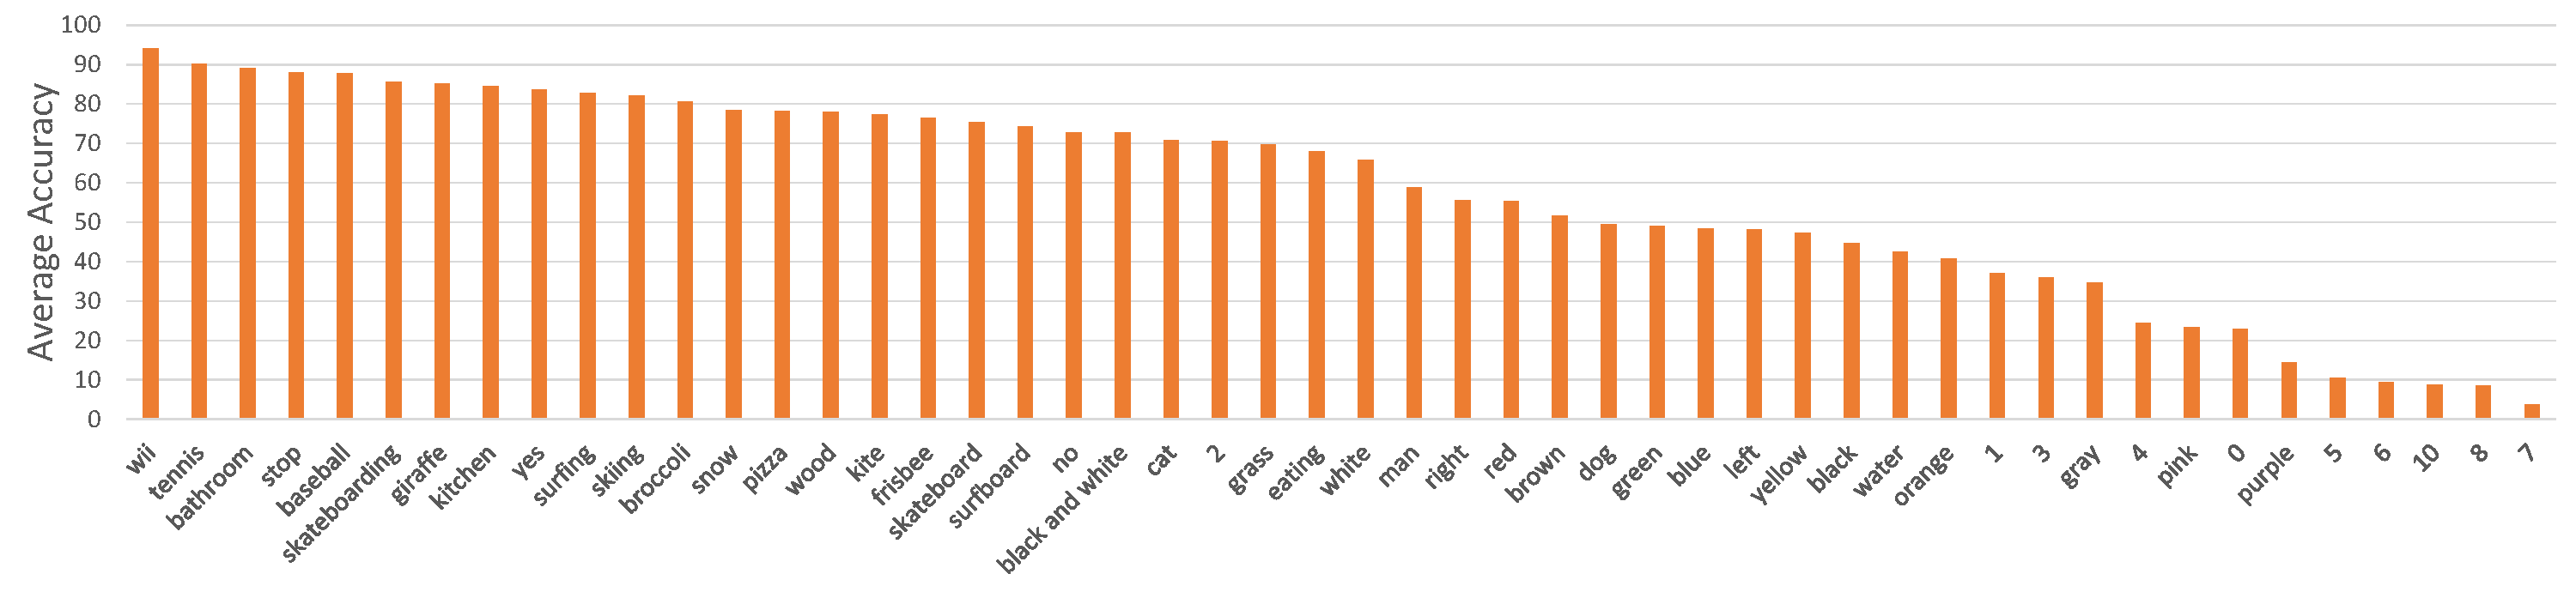
\includegraphics[width=1\linewidth]{figures/prob1_OpenEnded_val2014_sorted.pdf}
\centering
\caption{$\Pr\text{(system is correct } | \text{ answer)}$ for 50 most frequent ground truth answers on the VQA validation set (plot is sorted by accuracy, not frequency). System refers to our best model (deeper LSTM Q + norm I).}
\label{fig:prob_1}
%\vspace{\captionReduceBot}
\end{figure*}
\begin{figure*}[h]
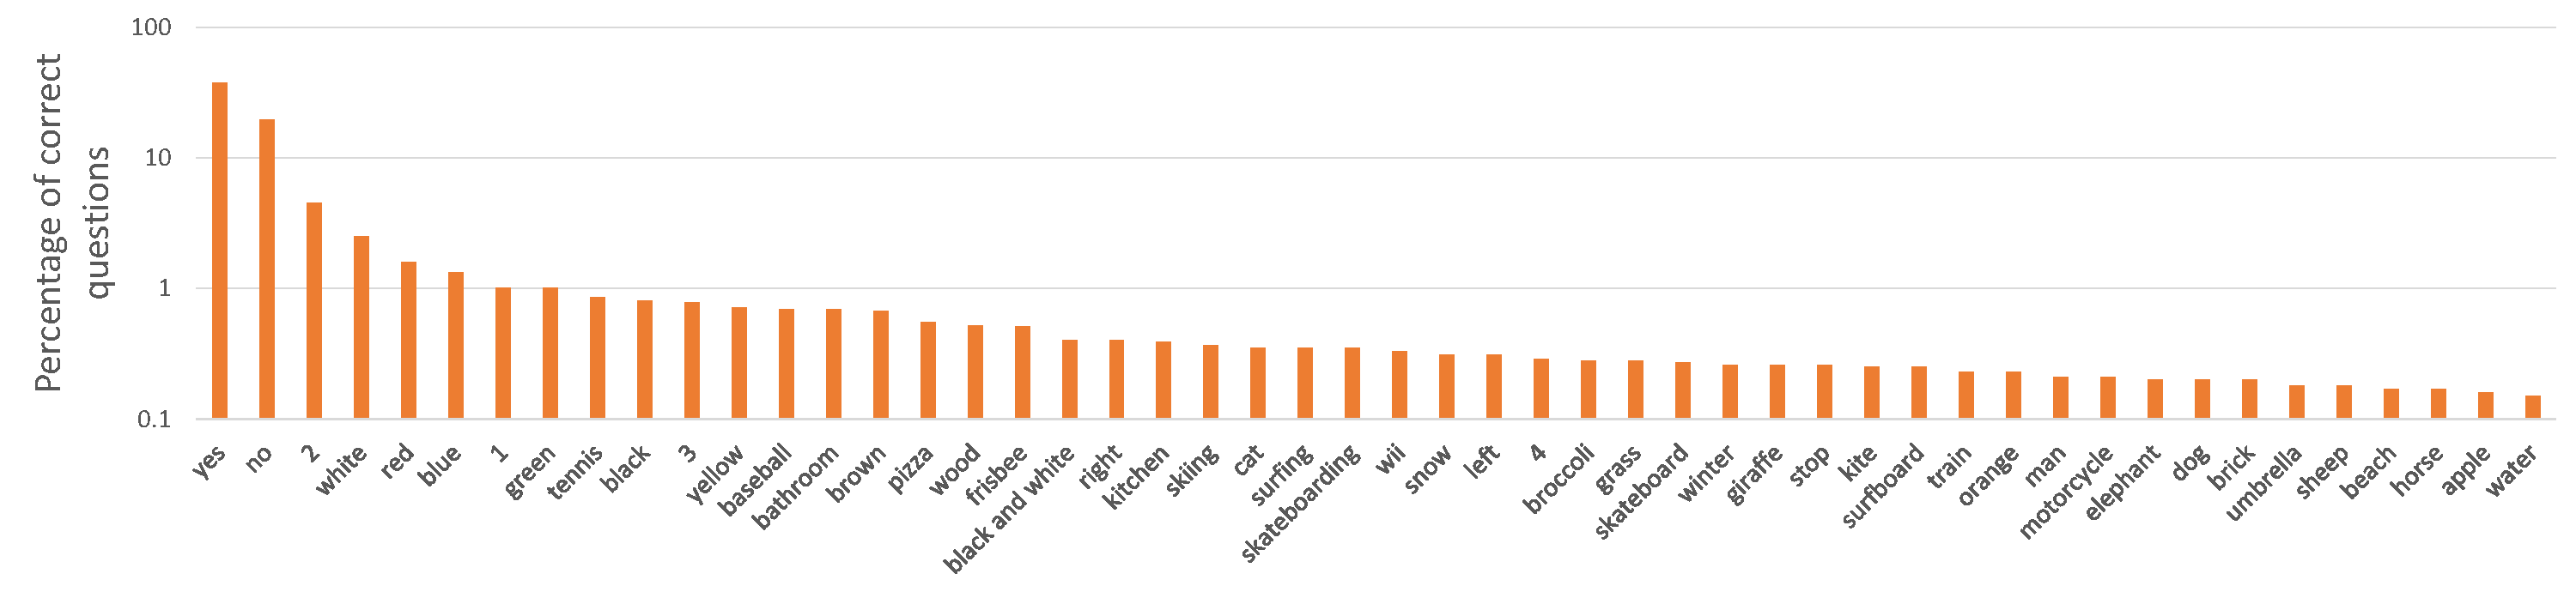
\includegraphics[width=1\linewidth]{figures/prob2_OpenEnded_val2014_100_logscale.pdf}
\centering
\caption{$\Pr\text{(answer } | \text{ system is correct)}$ for 50 most frequently predicted answers on the VQA validation set (plot is sorted by prediction frequency, not accuracy). System refers to our best model (deeper LSTM Q + norm I).}
\label{fig:prob_2}
%\vspace{\captionReduceBot}
\end{figure*}
\begin{figure}[h]
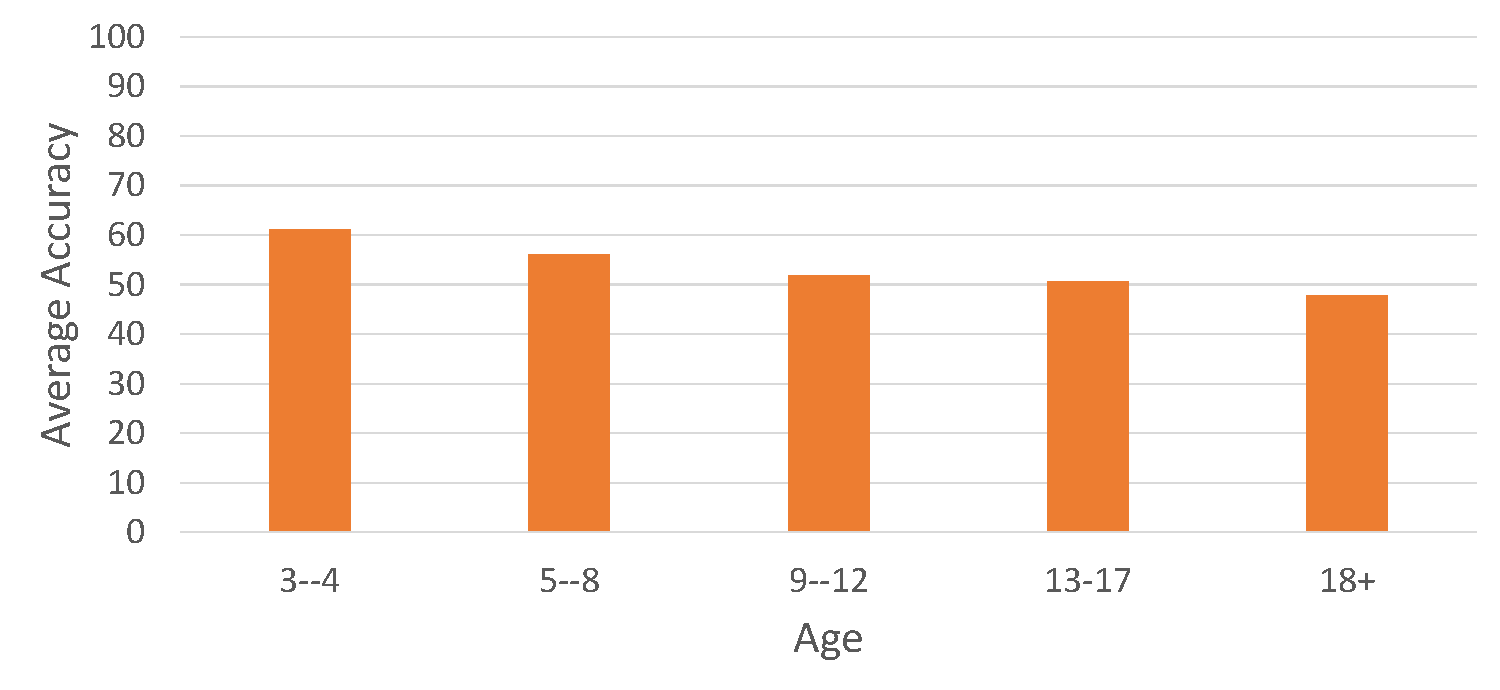
\includegraphics[width=1\linewidth]{figures/OpenEnded_val2014_predAgeDict2.pdf}
\centering
\caption{$\Pr\text{(system is correct } | \text{ age of question)}$ on the VQA validation set. System refers to our best model (deeper LSTM Q + norm I).}
\label{fig:age_1}
%\vspace{\captionReduceBot}
\end{figure}
\begin{figure}[h]
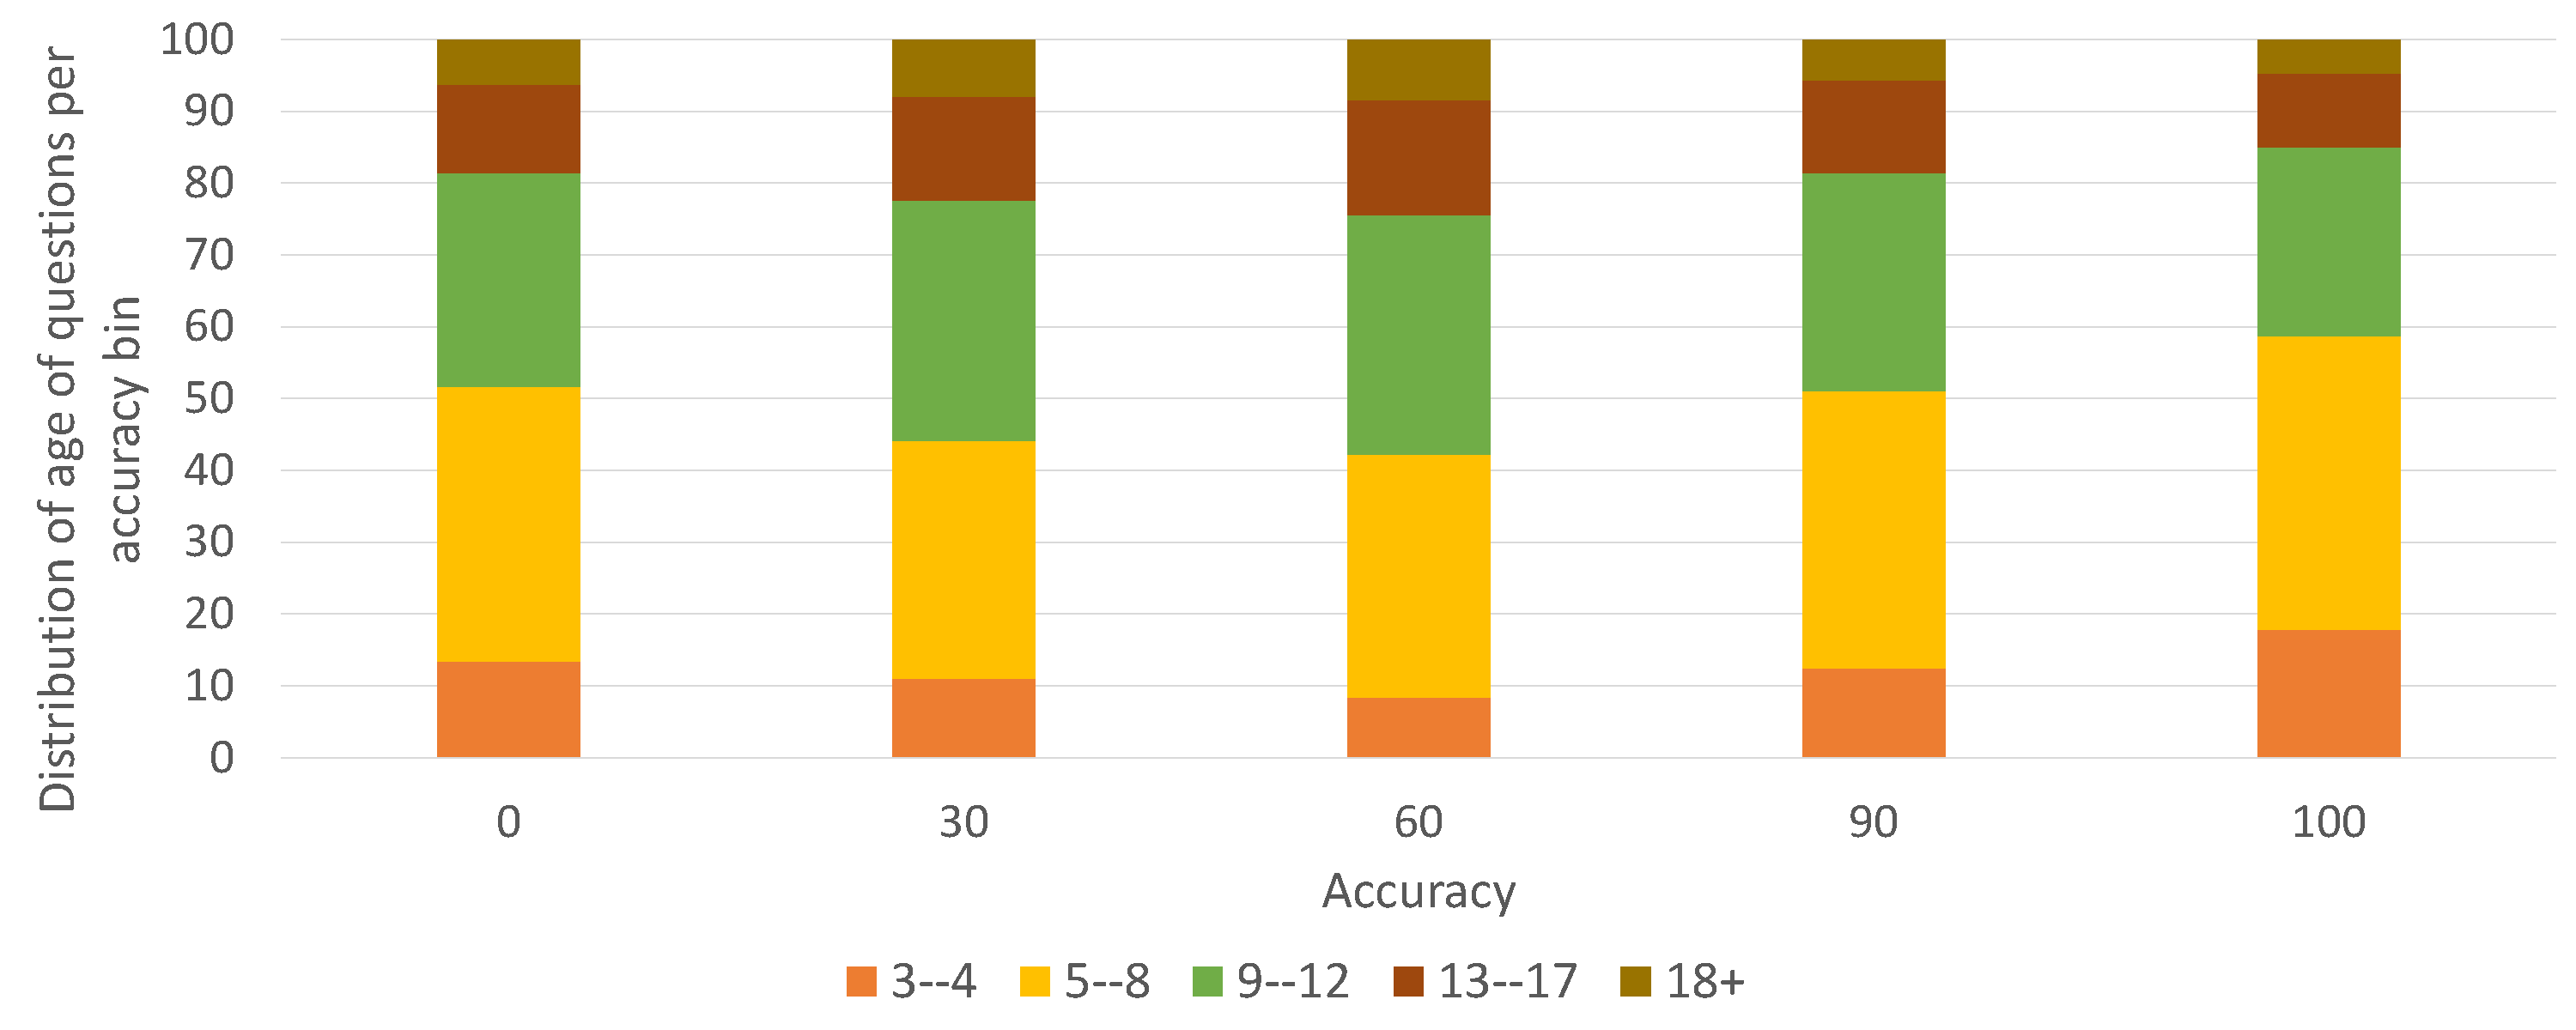
\includegraphics[width=1\linewidth]{figures/OpenEnded_val2014_predAgeDict1.pdf}
\centering
\caption{$\Pr\text{(age of question } | \text{ system is correct)}$ on the VQA validation set. System refers to our best model (deeper LSTM Q + norm I).}
\label{fig:age_2}
%\vspace{\captionReduceBot}
\end{figure}

\tableref{tab:abl_acc} shows the accuracy of different ablated versions of our best model (deeper LSTM Q + norm I) for both the open-ended and multiple-choice tasks on the VQA test-dev for real images. The different ablated versions are as follows --

\begin{compactenum}
\item \textbf{Without I Norm:} In this model, the activations from the last hidden layer of VGGNet~\cite{Simonyan14c} are not $\ell_2$-normalized. Comparing the accuracies in \tableref{tab:abl_acc} and \tableref{tab:acc}, we can see that $\ell_2$-normalization of image features boosts the performance by 0.16\% for open-ended task and by 0.24\% for multiple-choice task. 

\item \textbf{Concatenation:} In this model, the transformed image and LSTM embeddings are concatenated (instead of element-wise multiplied), resulting in doubling the number of parameters in the following fully-connected layer. Comparing the accuracies in \tableref{tab:abl_acc} and \tableref{tab:acc}, we can see that element-wise fusion performs better by 0.95\% for open-ended task and by 1.24\% for multiple-choice task.

\item \textbf{K = 500:} In this model, we use K = 500 most frequent answers as possible outputs. Comparing the accuracies in \tableref{tab:abl_acc} and \tableref{tab:acc}, we can see that K = 1000 performs better than K = 500 by 0.82\% for open-ended task and by 1.92\% for multiple-choice task.

\item \textbf{K = 2000:} In this model, we use K = 2000 most frequent answers as possible outputs. Comparing the accuracies in \tableref{tab:abl_acc} and \tableref{tab:acc}, we can see that K = 2000 performs better then K = 1000 by 0.40\% for open-ended task and by 1.16\% for multiple-choice task.

\item \textbf{Truncated Q Vocab $@$ 5:} In this model, the input vocabulary to the embedding layer (which encodes the question words) consists of only those question words which occur atleast 5 times in the training dataset, thus reducing the vocabulary size from 14770 (when all question words are used) to 5134 (65.24\% reduction). Remaining question words are replaced with UNK (unknown) tokens. Comparing the accuracies in \tableref{tab:abl_acc} and \tableref{tab:acc}, we can see that truncating the question vocabulary $@$ 5 performs better than using all questions words by 0.24\% for open-ended task and by 0.17\% for multiple-choice task.

\item \textbf{Truncated Q Vocab $@$ 11:} In this model, the input vocabulary to the embedding layer (which encodes the question words) consists of only those question words which occur atleast 11 times in the training dataset, thus reducing the vocabulary size from 14770 (when all question words are used) to 3561 (75.89\% reduction). Remaining question words are replaced with UNK (unknown) tokens. Comparing the accuracies in \tableref{tab:abl_acc} and \tableref{tab:acc}, we can see that truncating the question vocabulary $@$ 11 performs better than using all questions words by 0.06\% for open-ended task and by 0.02\% for multiple-choice task.

\item \textbf{Filtered Dataset:} We created a filtered version of the VQA train + val dataset in which we only keep the answers with subject confidence ``yes''. Also, we keep only those questions for which at least 50\% (5 out of 10) answers are annotated with subject confidence ``yes''. The resulting filtered dataset consists of 344600 questions, compared to 369861 questions in the original dataset, thus leading to only 6.83\% reduction in the size of the dataset. The filtered dataset has 8.77 answers per question on average. We did not filter the test set so that accuracies of the model trained on the filtered dataset can be compared with that of the model trained on the original dataset. The row ``Filtered Dataset'' in \tableref{tab:abl_acc} shows the performance of the deeper LSTM Q + norm I model when trained on the filtered dataset. Comparing these accuracies with the corresponding accuracies in \tableref{tab:acc}, we can see that the model trained on filtered version performs worse by 1.13\% for open-ended task and by 1.88\% for multiple-choice task.
\end{compactenum}

\begin{table}[t] \scriptsize
\setlength{\tabcolsep}{1.8pt}
\begin{center}
\begin{tabular}{@{} l  c  c  c  c  c  c c c@{}}
%\hline
\toprule
& \multicolumn{4}{c}{Open-Ended} & \multicolumn{4}{c}{Multiple-Choice} \\

\cmidrule[0.75pt](l){2-5}
\cmidrule[0.75pt](l){6-9}
 & All & Yes/No & Number & Other & All & Yes/No & Number & Other \\
%\hline
\midrule
Without I Norm & 57.59 & 80.41 & 36.63 & 42.84 & 62.46 & 80.43 & 38.10 & 52.62 \\
Concatenation & 56.80 & 78.49 & 35.08 & 43.19 & 61.46 & 78.52 & 36.43 & 52.54 \\
K = 500 & 56.93 & 80.61 & 36.24 & 41.39 & 60.78 & 80.64 & 37.44 & 49.10 \\
K = 2000 & 58.15 & 80.56 & 37.04 & 43.79 & 63.86 & 80.59 & 38.97 & 55.20 \\
Truncated Q Vocab $@$ 5 & 57.99 & 80.67 & 36.99 & 43.38 & 62.87 & 80.71 & 38.22 & 53.20\\
Truncated Q Vocab $@$ 11 & 57.81 & 80.42 & 36.97 & 43.22 & 62.72 & 80.45 & 38.30 & 53.09\\
Filtered Dataset & 56.62 & 80.19 & 37.48 & 40.95 & 60.82 & 80.19 & 37.48 & 49.57 \\
\bottomrule
\end{tabular}	
\caption{Accuracy of ablated versions of our best model (deeper LSTM Q + norm I) for the open-ended and multiple-choice tasks on the VQA test-dev for real images. 
Q = Question, I = Image. 
See text for details.
}
%\vspace{-10pt}
\label{tab:abl_acc}
\end{center}
\end{table}

\section{Experiments}
\label{sec:experiments}
\section{Experiments}
\label{sect:experiments}

% \begin{figure*}
%   \centering
%   \setlength{\tabcolsep}{0pt}
%   \setlength\figurewidth{0.05\textwidth}
%   \newcommand{\example}[1]{\raisebox{-.4\height}{\includegraphics[width=\figurewidth]{./figures/domains_examples/#1}}}
%   \begin{sc}
%   \begin{tabular}{r@{\hskip 1cm} ccccccccccc}
%     MNIST \cite{LeCun98} &
%     \example{mnist_0.png} &
%     \example{mnist_1.png} &
%     \example{mnist_2.png} &
%     \example{mnist_3.png} &
%     \example{mnist_4.png} &
%     \example{mnist_5.png} &
%     \example{mnist_6.png} &
%     \example{mnist_7.png} &
%     \example{mnist_8.png} &
%     \example{mnist_9.png} &
%     \example{mnist_10.png}\\
%     MNIST ($ | \Delta | $, BG) &
%     \example{mnisti_0.png} &
%     \example{mnisti_1.png} &
%     \example{mnisti_2.png} &
%     \example{mnisti_3.png} &
%     \example{mnisti_4.png} &
%     \example{mnisti_5.png} &
%     \example{mnisti_6.png} &
%     \example{mnisti_7.png} &
%     \example{mnisti_8.png} &
%     \example{mnisti_9.png} &
%     \example{mnisti_10.png}\\
%     Syn Numbers &
%     \example{syn_0.png} &
%     \example{syn_1.png} &
%     \example{syn_2.png} &
%     \example{syn_3.png} &
%     \example{syn_4.png} &
%     \example{syn_5.png} &
%     \example{syn_6.png} &
%     \example{syn_7.png} &
%     \example{syn_8.png} &
%     \example{syn_9.png} &
%     \example{syn_10.png}\\
%     SVHN \cite{Netzer11} &
%     \example{svhn_0.png} &
%     \example{svhn_1.png} &
%     \example{svhn_2.png} &
%     \example{svhn_3.png} &
%     \example{svhn_4.png} &
%     \example{svhn_5.png} &
%     \example{svhn_6.png} &
%     \example{svhn_7.png} &
%     \example{svhn_8.png} &
%     \example{svhn_9.png} &
%     \example{svhn_10.png}\\
%     Syn Signs &
%     \example{synsgn_11.png} &
%     \example{synsgn_1.png} &
%     \example{synsgn_2.png} &
%     \example{synsgn_3.png} &
%     \example{synsgn_4.png} &
%     \example{synsgn_5.png} &
%     \example{synsgn_12.png} &
%     \example{synsgn_7.png} &
%     \example{synsgn_8.png} &
%     \example{synsgn_9.png} &
%     \example{synsgn_10.png}\\
%     GTSRB \cite{Stallkamp12} &
%     \example{gtsrb_0.png} &
%     \example{gtsrb_1.png} &
%     \example{gtsrb_2.png} &
%     \example{gtsrb_3.png} &
%     \example{gtsrb_4.png} &
%     \example{gtsrb_5.png} &
%     \example{gtsrb_6.png} &
%     \example{gtsrb_7.png} &
%     \example{gtsrb_8.png} &
%     \example{gtsrb_9.png} &
%     \example{gtsrb_10.png}\\
%     % CIFAR-10 \cite{Krizhevsky09} &
%     % \example{cifar10_0.png} &
%     % \example{cifar10_1.png} &
%     % \example{cifar10_2.png} &
%     % \example{cifar10_3.png} &
%     % \example{cifar10_4.png} &
%     % \example{cifar10_5.png} &
%     % \example{cifar10_11.png} &
%     % \example{cifar10_7.png} &
%     % \example{cifar10_8.png} &
%     % \example{cifar10_9.png} &
%     % \example{cifar10_10.png}\\
%     % STL-10 \cite{Coates11} &
%     % \example{stl10_12.png} &
%     % \example{stl10_1.png} &
%     % \example{stl10_2.png} &
%     % \example{stl10_3.png} &
%     % \example{stl10_4.png} &
%     % \example{stl10_5.png} &
%     % \example{stl10_6.png} &
%     % \example{stl10_13.png} &
%     % \example{stl10_8.png} &
%     % \example{stl10_9.png} &
%     % \example{stl10_10.png}\\
%   \end{tabular}
%   \end{sc}
%   \vskip 2.5mm
%   \caption{\todo[What to do with this figure? Add Office? Remove?]Random samples from the datasets used in the experiments. See \sect{exper_quant} for details.}
%   \label{fig:exper_domains_examples}
% \end{figure*}

\begin{figure*}
  \centering
  \setlength{\tabcolsep}{0pt}
  \setlength\figurewidth{0.05\textwidth}
  \newcommand{\example}[1]{\raisebox{-.4\height}{\includegraphics[width=\figurewidth]{./figures/domains_examples/#1}}}
  \begin{sc}
  \begin{small}
  \begin{tabular}{r@{\hskip 0.5cm} ccc c@{\hskip 0.4cm} ccc c@{\hskip 0.4cm} ccc c@{\hskip 0.4cm} ccc}
    &
    \multicolumn{3}{c}{MNIST} & &
    \multicolumn{3}{c}{Syn Numbers} & &
    \multicolumn{3}{c}{SVHN} & &
    \multicolumn{3}{c}{Syn Signs}\\
    
    Source &
    \example{mnist_0.png} &
    \example{mnist_1.png} &
    \example{mnist_3.png} & &
    
    \example{syn_0.png} &
    \example{syn_1.png} &
    \example{syn_2.png} & &
    
    \example{svhn_3.png} &
    \example{svhn_4.png} &
    \example{svhn_5.png} & &
    
    \example{synsgn_3.png} &
    \example{synsgn_4.png} &
    \example{synsgn_5.png}\\
    
    Target &
    \example{mnisti_0.png} &
    \example{mnisti_1.png} &
    \example{mnisti_2.png} & &
    
    \example{svhn_0.png} &
    \example{svhn_1.png} &
    \example{svhn_2.png} & &
    
    \example{mnist_4.png} &
    \example{mnist_5.png} &
    \example{mnist_6.png} & &
    
    \example{gtsrb_2.png} &
    \example{gtsrb_3.png} &
    \example{gtsrb_4.png}\\
    
    &
    \multicolumn{3}{c}{\rule{0pt}{0.35cm} MNIST-M} & &
    \multicolumn{3}{c}{SVHN} & &
    \multicolumn{3}{c}{MNIST} & &
    \multicolumn{3}{c}{GTSRB}\\
  \end{tabular}
  \end{small}
  \end{sc}
  \caption{Examples of domain pairs used in the experiments. See \sect{exper_quant} for details.}
  \label{fig:exper_domains_examples}
\end{figure*}


\begin{table*}[t]
  \vskip 0.15in
  \begin{center}
    \begin{small}
      \begin{sc}
        \renewcommand{\arraystretch}{1.5}
        \begin{tabular}{l r | c c c c}
          \hline
          \multirow{2}{*}{Method} & {\scriptsize Source} & MNIST & Syn Numbers & SVHN & Syn Signs \\
          & {\scriptsize Target} & MNIST-M & SVHN & MNIST & GTSRB \\
          \hline
          \multicolumn{2}{l |}{Source only} & 
          $ .5749 $                      & $ .8665 $                      & $ .5919 $                      & $ .7400 $                      \\
          \multicolumn{2}{l |}{SA \cite{Fernando13}} & 
          $ .6078 \; (7.9\%) $           & $ .8672 \; (1.3\%) $           & $ .6157 \; (5.9\%) $           & $ .7635 \; (9.1\%) $           \\
          \multicolumn{2}{l |}{Proposed approach} & 
          $ \mathbf{.8149} \; (57.9\%) $ & $ \mathbf{.9048} \; (66.1\%) $ & $ \mathbf{.7107} \; (29.3\%) $ & $ \mathbf{.8866} \; (56.7\%) $ \\
          \multicolumn{2}{l |}{Train on target} & 
          $ .9891 $                      & $ .9244 $                      & $ .9951 $                      & $ .9987 $                      \\
          \hline
        \end{tabular}
      \end{sc}
    \end{small}
  \end{center}
    \caption{Classification accuracies for digit image classifications for different source and target domains. {\sc MNIST-M} corresponds to difference-blended digits over non-uniform background. The first row corresponds to the lower performance bound (i.e.\ if no adaptation is performed). The last row corresponds to training on the target domain data with known class labels (upper bound on the DA performance). For each of the two DA methods (ours and \cite{Fernando13}) we show how much of the gap between the lower and the upper bounds was covered (in brackets). For all five cases, our approach outperforms \cite{Fernando13} considerably, and covers a big portion of the gap.\vspace{-0mm} }
  \label{tab:results}
  \vskip -0.1in
\end{table*}

\begin{table*}[t]
  \vskip 0.15in
  \begin{center}
    \begin{small}
      \begin{sc}
        \renewcommand{\arraystretch}{1.5}
        \begin{tabular}{l r | c c c}
          \hline
          \multirow{2}{*}{Method} & {\scriptsize Source} & Amazon & DSLR & Webcam \\
          & {\scriptsize Target} & Webcam & Webcam & DSLR \\
          \hline
          \multicolumn{2}{l |}{GFK(PLS, PCA) \cite{Gong12}} & 
          $ .464 \pm .005 $ & $ .613 \pm .004 $ & $ .663 \pm .004 $\\ 
          \multicolumn{2}{l |}{SA \cite{Fernando13}} & 
          $ .450 $ & $ .648 $ & $ .699 $\\ 
          \multicolumn{2}{l |}{DA-NBNN \cite{Tommasi13}} & 
          $ .528 \pm .037 $ & $ .766 \pm .017 $ & $ .762 \pm .025 $\\ 
          \multicolumn{2}{l |}{DLID \cite{Chopra13}} & 
          $ .519 $ & $ .782 $ & $ .899 $\\
          \multicolumn{2}{l |}{DeCAF$_6$ Source Only \cite{Donahue14}} &
          $ .522 \pm .017 $ & $ .915 \pm .015 $ & --\\ 
          \multicolumn{2}{l |}{DaNN \cite{Ghifary14}} & 
          $ .536 \pm .002 $ & $ .712 \pm .000 $ & $ .835 \pm .000 $\\ 
          \multicolumn{2}{l |}{DDC \cite{Tzeng14}} & 
          $ .594 \pm .008 $ & $ .925 \pm .003 $ & $ .917 \pm .008 $\\ 
          \multicolumn{2}{l |}{Proposed Approach} & 
          $ \mathbf{ .673 \pm .017 } $ & $ \mathbf{ .940 \pm .008 } $ & $ \mathbf{ .937 \pm .010 } $\\
          \hline
        \end{tabular}
      \end{sc}
    \end{small}
  \end{center}
    \caption{Accuracy evaluation of different DA approaches on the standard {\sc Office} \cite{Saenko10} dataset. Our method (last row) outperforms competitors setting the new state-of-the-art.}
  \label{tab:results_office}
\end{table*}

% Other rows refer to the following algorithms (from top to bottom): Geodesic Flow Kernel \cite{Gong12}, Subspace Alignment \cite{Fernando13}, Naive Bayes Nearest Neighbor \cite{Tommasi13},  deep learning approach from \cite{Chopra13}, DeCAF$_6$-features described in \cite{Donahue14}, Domain Adaptive NNs \cite{Ghifary14}, Deep Domain Confusion \cite{Tzeng14}.

\def\X{{\mathbf X}}
\def\y{{\mathbf y}}

% \vspace{2mm}\noindent {\bf Datasets.}
% \label{sect:exper_datasets}

% In order to test our method in the setting of traffic signs classification we obtained~100,000 synthetic images ({\sc Syn~Signs}) simulating various photoshooting conditions. This dataset was used in conjunction with {\it The German Traffic Sign Recognition Benchmark} ({\sc GTSRB}) \cite{Stallkamp12}.

% Finally, we perform domain adaption for the {\sc CIFAR-10} and the {\sc STL-10} downsampled to the size of $ 32 \times 32 $. This pair is considerably different from the previously mentioned datasets as the intra-class variability here is higher.

We perform extensive evaluation of the proposed approach on a number of popular image datasets and their modifications. These include large-scale datasets of small images popular with deep learning methods, and the {\sc Office} datasets \cite{Saenko10}, which are a {\em de facto} standard for domain adaptation in computer vision, but have much fewer images.

\vspace{2mm}\noindent {\bf Baselines.} For the bulk of experiments the following baselines are evaluated. The \textbf{source-only} model is trained without consideration for target-domain data (no domain classifier branch included into the network). The \textbf{train-on-target} model is trained on the target domain with class labels revealed. This model serves as an upper bound on DA methods, assuming that target data are abundant and the shift between the domains is considerable. 

In addition, we compare our approach against the recently proposed unsupervised DA method based on \textbf{subspace alignment (SA)} \cite{Fernando13}, which is simple to setup and test on new datasets, but has also been shown to perform very well in experimental comparisons with other ``shallow'' DA methods. To boost the performance of this baseline, we pick its most important free parameter (the number of principal components) from the range $ \{ 2, \ldots, 60 \} $, so that the test performance on the target domain is maximized. To apply SA in our setting, we train a source-only model and then consider the activations of the last hidden layer in the label predictor (before the final linear classifier) as descriptors/features, and learn the mapping between the source and the target domains \cite{Fernando13}.

Since the SA baseline requires to train a new classifier after adapting the features, and in order to put all the compared settings on an equal footing, we retrain the last layer of the label predictor using a standard linear SVM~\cite{liblinear} for all four considered methods (including ours; the performance on the target domain remains approximately the same after the retraining). 

For the {\sc Office} dataset \cite{Saenko10}, we directly compare the performance of our full network (feature extractor and label predictor) against recent DA approaches using previously published results.

\vspace{2mm}\noindent {\bf CNN architectures.} In general, we compose feature extractor from two or three convolutional layers, picking their exact configurations from previous works. We give the exact architectures in \ref{sect:appendix_archs}.

For the domain adaptator we stick to the three fully connected layers ($x\rightarrow1024\rightarrow1024\rightarrow2$), except for {\sc MNIST} where we used a simpler ($x\rightarrow100\rightarrow2$) architecture to speed up the experiments.

For loss functions, we set $ L_y $ and $ L_d $ to be the logistic regression loss and the binomial cross-entropy respectively.

\vspace{2mm}\noindent {\bf CNN training procedure.}
The model is trained on $128$-sized batches. Images are preprocessed by the mean subtraction. A half of each batch is populated by the samples from the source domain (with known labels), the rest is comprised of the target domain (with unknown labels).

In order to suppress noisy signal from the domain classifier at the early stages of the training procedure instead of fixing the adaptation factor $ \lambda $, we gradually change it from $0$ to $1$ using the following schedule:
\begin{equation}
  \lambda_p = \frac{2}{1 + \exp(-\gamma \cdot p)} - 1,
\end{equation}
where $\gamma$ was set to $10$ in all experiments (the schedule was not optimized/tweaked). Further details on the CNN training can be found in \ref{sect:appendix_training}.

\vspace{2mm}\noindent {\bf Visualizations.}
We use t-SNE \cite{Maaten13} projection to visualize feature distributions at different points of the network, while color-coding the domains (\fig{exper_adapt_vis}). We observe strong correspondence between the success of the adaptation in terms of the classification accuracy for the target domain, and the overlap between the domain distributions in such visualizations.
 
\vspace{2mm}\noindent {\bf Choosing meta-parameters.} 
In general, good unsupervised DA methods should provide ways to set meta-parameters (such as $\lambda$, the learning rate, the momentum rate, the network architecture for our method) in an unsupervised way, i.e.\ without referring to labeled data in the target domain. %Here we would like to give few recommendations concerning this matter. First, as it was pointed out in \sect{theory} the domain classifier should not be significantly more complex than the label predictor. 
In our method, one can assess the performance of the whole system (and the effect of changing hyper-parameters) by observing the test error on the source domain {\em and} the domain classifier error. In general, we observed a good correspondence between the success of adaptation and these errors (adaptation is more successful when the source domain test error is low, while the domain classifier error is high).
In addition, the layer, where the the domain adaptator is attached can be picked by computing difference between means as suggested in \cite{Tzeng14}. 

% \begin{figure*}
%   \centering
%   {\sc MNIST $ \rightarrow $ MNIST ($ | \Delta | $, bg)}: top feature extractor layer
%   \setcounter{subfigure}{0}
%   \subfigure[Non-adapted]{%%
%     \scalebox{0.8}{%% Creator: Matplotlib, PGF backend
%%
%% To include the figure in your LaTeX document, write
%%   \input{<filename>.pgf}
%%
%% Make sure the required packages are loaded in your preamble
%%   \usepackage{pgf}
%%
%% Figures using additional raster images can only be included by \input if
%% they are in the same directory as the main LaTeX file. For loading figures
%% from other directories you can use the `import` package
%%   \usepackage{import}
%% and then include the figures with
%%   \import{<path to file>}{<filename>.pgf}
%%
%% Matplotlib used the following preamble
%%   \usepackage[utf8x]{inputenc}
%%   \usepackage[T1]{fontenc}
%%
\begingroup%
\makeatletter%
\begin{pgfpicture}%
\pgfpathrectangle{\pgfpointorigin}{\pgfqpoint{3.338520in}{2.040000in}}%
\pgfusepath{use as bounding box}%
\begin{pgfscope}%
\pgfsetbuttcap%
\pgfsetroundjoin%
\definecolor{currentfill}{rgb}{1.000000,1.000000,1.000000}%
\pgfsetfillcolor{currentfill}%
\pgfsetlinewidth{0.000000pt}%
\definecolor{currentstroke}{rgb}{1.000000,1.000000,1.000000}%
\pgfsetstrokecolor{currentstroke}%
\pgfsetdash{}{0pt}%
\pgfpathmoveto{\pgfqpoint{0.000000in}{-0.000000in}}%
\pgfpathlineto{\pgfqpoint{3.338520in}{-0.000000in}}%
\pgfpathlineto{\pgfqpoint{3.338520in}{2.040000in}}%
\pgfpathlineto{\pgfqpoint{0.000000in}{2.040000in}}%
\pgfpathclose%
\pgfusepath{fill}%
\end{pgfscope}%
\begin{pgfscope}%
\pgftext[at=\pgfqpoint{0.510000in}{0.348333in},left,bottom]{\pgfimage[interpolate=true,width=2.553333in,height=1.500000in]{./figures/adaptation_vis/pool2_mnist2inv_before-img0.png}}%
\end{pgfscope}%
\begin{pgfscope}%
\pgftext[at=\pgfqpoint{0.805000in}{0.383333in},left,bottom]{\pgfimage[interpolate=true,width=2.201667in,height=1.371667in]{./figures/adaptation_vis/pool2_mnist2inv_before-img1.png}}%
\end{pgfscope}%
\end{pgfpicture}%
\makeatother%
\endgroup%
}}%%
%   \subfigure[Adapted]{%%
%     \scalebox{0.8}{%% Creator: Matplotlib, PGF backend
%%
%% To include the figure in your LaTeX document, write
%%   \input{<filename>.pgf}
%%
%% Make sure the required packages are loaded in your preamble
%%   \usepackage{pgf}
%%
%% Figures using additional raster images can only be included by \input if
%% they are in the same directory as the main LaTeX file. For loading figures
%% from other directories you can use the `import` package
%%   \usepackage{import}
%% and then include the figures with
%%   \import{<path to file>}{<filename>.pgf}
%%
%% Matplotlib used the following preamble
%%   \usepackage[utf8x]{inputenc}
%%   \usepackage[T1]{fontenc}
%%
\begingroup%
\makeatletter%
\begin{pgfpicture}%
\pgfpathrectangle{\pgfpointorigin}{\pgfqpoint{3.340000in}{2.040000in}}%
\pgfusepath{use as bounding box}%
\begin{pgfscope}%
\pgfsetbuttcap%
\pgfsetroundjoin%
\definecolor{currentfill}{rgb}{1.000000,1.000000,1.000000}%
\pgfsetfillcolor{currentfill}%
\pgfsetlinewidth{0.000000pt}%
\definecolor{currentstroke}{rgb}{1.000000,1.000000,1.000000}%
\pgfsetstrokecolor{currentstroke}%
\pgfsetdash{}{0pt}%
\pgfpathmoveto{\pgfqpoint{0.000000in}{-0.000000in}}%
\pgfpathlineto{\pgfqpoint{3.340000in}{-0.000000in}}%
\pgfpathlineto{\pgfqpoint{3.340000in}{2.040000in}}%
\pgfpathlineto{\pgfqpoint{0.000000in}{2.040000in}}%
\pgfpathclose%
\pgfusepath{fill}%
\end{pgfscope}%
\begin{pgfscope}%
\pgftext[at=\pgfqpoint{0.518333in}{0.321667in},left,bottom]{\pgfimage[interpolate=true,width=2.565000in,height=1.550000in]{./figures/adaptation_vis/pool2_mnist2inv_after-img0.png}}%
\end{pgfscope}%
\begin{pgfscope}%
\pgftext[at=\pgfqpoint{0.518333in}{0.321667in},left,bottom]{\pgfimage[interpolate=true,width=2.565000in,height=1.553333in]{./figures/adaptation_vis/pool2_mnist2inv_after-img1.png}}%
\end{pgfscope}%
\end{pgfpicture}%
\makeatother%
\endgroup%
}}\\
%   \vspace{5mm}
%   {\sc Syn Numbers $ \rightarrow $ SVHN}: last hidden layer of the label predictor
%   \setcounter{subfigure}{0}
%   \subfigure[Non-adapted]{%%
%     \scalebox{0.8}{%% Creator: Matplotlib, PGF backend
%%
%% To include the figure in your LaTeX document, write
%%   \input{<filename>.pgf}
%%
%% Make sure the required packages are loaded in your preamble
%%   \usepackage{pgf}
%%
%% Figures using additional raster images can only be included by \input if
%% they are in the same directory as the main LaTeX file. For loading figures
%% from other directories you can use the `import` package
%%   \usepackage{import}
%% and then include the figures with
%%   \import{<path to file>}{<filename>.pgf}
%%
%% Matplotlib used the following preamble
%%   \usepackage[utf8x]{inputenc}
%%   \usepackage[T1]{fontenc}
%%
\begingroup%
\makeatletter%
\begin{pgfpicture}%
\pgfpathrectangle{\pgfpointorigin}{\pgfqpoint{3.340000in}{2.040000in}}%
\pgfusepath{use as bounding box}%
\begin{pgfscope}%
\pgfsetbuttcap%
\pgfsetroundjoin%
\definecolor{currentfill}{rgb}{1.000000,1.000000,1.000000}%
\pgfsetfillcolor{currentfill}%
\pgfsetlinewidth{0.000000pt}%
\definecolor{currentstroke}{rgb}{1.000000,1.000000,1.000000}%
\pgfsetstrokecolor{currentstroke}%
\pgfsetdash{}{0pt}%
\pgfpathmoveto{\pgfqpoint{0.000000in}{-0.000000in}}%
\pgfpathlineto{\pgfqpoint{3.340000in}{-0.000000in}}%
\pgfpathlineto{\pgfqpoint{3.340000in}{2.040000in}}%
\pgfpathlineto{\pgfqpoint{0.000000in}{2.040000in}}%
\pgfpathclose%
\pgfusepath{fill}%
\end{pgfscope}%
\begin{pgfscope}%
\pgftext[at=\pgfqpoint{0.491667in}{0.335000in},left,bottom]{\pgfimage[interpolate=true,width=2.618333in,height=1.531667in]{./figures/adaptation_vis/before-img0.png}}%
\end{pgfscope}%
\begin{pgfscope}%
\pgftext[at=\pgfqpoint{0.758333in}{0.331667in},left,bottom]{\pgfimage[interpolate=true,width=2.171667in,height=1.436667in]{./figures/adaptation_vis/before-img1.png}}%
\end{pgfscope}%
\begin{pgfscope}%
\pgfsetbuttcap%
\pgfsetroundjoin%
\definecolor{currentfill}{rgb}{0.000000,0.000000,1.000000}%
\pgfsetfillcolor{currentfill}%
\pgfsetfillopacity{0.300000}%
\pgfsetlinewidth{0.150562pt}%
\definecolor{currentstroke}{rgb}{0.000000,0.000000,0.000000}%
\pgfsetstrokecolor{currentstroke}%
\pgfsetstrokeopacity{0.300000}%
\pgfsetdash{}{0pt}%
\pgfpathmoveto{\pgfqpoint{2.521160in}{1.775861in}}%
\pgfpathcurveto{\pgfqpoint{2.525278in}{1.775861in}}{\pgfqpoint{2.529228in}{1.777497in}}{\pgfqpoint{2.532140in}{1.780409in}}%
\pgfpathcurveto{\pgfqpoint{2.535052in}{1.783321in}}{\pgfqpoint{2.536688in}{1.787271in}}{\pgfqpoint{2.536688in}{1.791389in}}%
\pgfpathcurveto{\pgfqpoint{2.536688in}{1.795507in}}{\pgfqpoint{2.535052in}{1.799457in}}{\pgfqpoint{2.532140in}{1.802369in}}%
\pgfpathcurveto{\pgfqpoint{2.529228in}{1.805281in}}{\pgfqpoint{2.525278in}{1.806917in}}{\pgfqpoint{2.521160in}{1.806917in}}%
\pgfpathcurveto{\pgfqpoint{2.517042in}{1.806917in}}{\pgfqpoint{2.513092in}{1.805281in}}{\pgfqpoint{2.510180in}{1.802369in}}%
\pgfpathcurveto{\pgfqpoint{2.507268in}{1.799457in}}{\pgfqpoint{2.505631in}{1.795507in}}{\pgfqpoint{2.505631in}{1.791389in}}%
\pgfpathcurveto{\pgfqpoint{2.505631in}{1.787271in}}{\pgfqpoint{2.507268in}{1.783321in}}{\pgfqpoint{2.510180in}{1.780409in}}%
\pgfpathcurveto{\pgfqpoint{2.513092in}{1.777497in}}{\pgfqpoint{2.517042in}{1.775861in}}{\pgfqpoint{2.521160in}{1.775861in}}%
\pgfpathclose%
\pgfusepath{stroke,fill}%
\end{pgfscope}%
\begin{pgfscope}%
\pgfsetbuttcap%
\pgfsetroundjoin%
\definecolor{currentfill}{rgb}{0.000000,0.000000,1.000000}%
\pgfsetfillcolor{currentfill}%
\pgfsetfillopacity{0.300000}%
\pgfsetlinewidth{0.150562pt}%
\definecolor{currentstroke}{rgb}{0.000000,0.000000,0.000000}%
\pgfsetstrokecolor{currentstroke}%
\pgfsetstrokeopacity{0.300000}%
\pgfsetdash{}{0pt}%
\pgfpathmoveto{\pgfqpoint{2.598938in}{1.785583in}}%
\pgfpathcurveto{\pgfqpoint{2.603056in}{1.785583in}}{\pgfqpoint{2.607006in}{1.787219in}}{\pgfqpoint{2.609918in}{1.790131in}}%
\pgfpathcurveto{\pgfqpoint{2.612830in}{1.793043in}}{\pgfqpoint{2.614466in}{1.796993in}}{\pgfqpoint{2.614466in}{1.801111in}}%
\pgfpathcurveto{\pgfqpoint{2.614466in}{1.805229in}}{\pgfqpoint{2.612830in}{1.809179in}}{\pgfqpoint{2.609918in}{1.812091in}}%
\pgfpathcurveto{\pgfqpoint{2.607006in}{1.815003in}}{\pgfqpoint{2.603056in}{1.816639in}}{\pgfqpoint{2.598938in}{1.816639in}}%
\pgfpathcurveto{\pgfqpoint{2.594819in}{1.816639in}}{\pgfqpoint{2.590869in}{1.815003in}}{\pgfqpoint{2.587957in}{1.812091in}}%
\pgfpathcurveto{\pgfqpoint{2.585045in}{1.809179in}}{\pgfqpoint{2.583409in}{1.805229in}}{\pgfqpoint{2.583409in}{1.801111in}}%
\pgfpathcurveto{\pgfqpoint{2.583409in}{1.796993in}}{\pgfqpoint{2.585045in}{1.793043in}}{\pgfqpoint{2.587957in}{1.790131in}}%
\pgfpathcurveto{\pgfqpoint{2.590869in}{1.787219in}}{\pgfqpoint{2.594819in}{1.785583in}}{\pgfqpoint{2.598938in}{1.785583in}}%
\pgfpathclose%
\pgfusepath{stroke,fill}%
\end{pgfscope}%
\begin{pgfscope}%
\pgfsetbuttcap%
\pgfsetroundjoin%
\definecolor{currentfill}{rgb}{0.000000,0.000000,1.000000}%
\pgfsetfillcolor{currentfill}%
\pgfsetfillopacity{0.300000}%
\pgfsetlinewidth{0.150562pt}%
\definecolor{currentstroke}{rgb}{0.000000,0.000000,0.000000}%
\pgfsetstrokecolor{currentstroke}%
\pgfsetstrokeopacity{0.300000}%
\pgfsetdash{}{0pt}%
\pgfpathmoveto{\pgfqpoint{2.676715in}{1.771000in}}%
\pgfpathcurveto{\pgfqpoint{2.680833in}{1.771000in}}{\pgfqpoint{2.684783in}{1.772636in}}{\pgfqpoint{2.687695in}{1.775548in}}%
\pgfpathcurveto{\pgfqpoint{2.690607in}{1.778460in}}{\pgfqpoint{2.692244in}{1.782410in}}{\pgfqpoint{2.692244in}{1.786528in}}%
\pgfpathcurveto{\pgfqpoint{2.692244in}{1.790646in}}{\pgfqpoint{2.690607in}{1.794596in}}{\pgfqpoint{2.687695in}{1.797508in}}%
\pgfpathcurveto{\pgfqpoint{2.684783in}{1.800420in}}{\pgfqpoint{2.680833in}{1.802056in}}{\pgfqpoint{2.676715in}{1.802056in}}%
\pgfpathcurveto{\pgfqpoint{2.672597in}{1.802056in}}{\pgfqpoint{2.668647in}{1.800420in}}{\pgfqpoint{2.665735in}{1.797508in}}%
\pgfpathcurveto{\pgfqpoint{2.662823in}{1.794596in}}{\pgfqpoint{2.661187in}{1.790646in}}{\pgfqpoint{2.661187in}{1.786528in}}%
\pgfpathcurveto{\pgfqpoint{2.661187in}{1.782410in}}{\pgfqpoint{2.662823in}{1.778460in}}{\pgfqpoint{2.665735in}{1.775548in}}%
\pgfpathcurveto{\pgfqpoint{2.668647in}{1.772636in}}{\pgfqpoint{2.672597in}{1.771000in}}{\pgfqpoint{2.676715in}{1.771000in}}%
\pgfpathclose%
\pgfusepath{stroke,fill}%
\end{pgfscope}%
\begin{pgfscope}%
\pgftext[x=2.798938in,y=1.762222in,left,base]{{\rmfamily\fontsize{8.000000}{9.600000}\selectfont Source}}%
\end{pgfscope}%
\begin{pgfscope}%
\pgfsetbuttcap%
\pgfsetroundjoin%
\definecolor{currentfill}{rgb}{1.000000,0.000000,0.000000}%
\pgfsetfillcolor{currentfill}%
\pgfsetfillopacity{0.300000}%
\pgfsetlinewidth{0.150562pt}%
\definecolor{currentstroke}{rgb}{0.000000,0.000000,0.000000}%
\pgfsetstrokecolor{currentstroke}%
\pgfsetstrokeopacity{0.300000}%
\pgfsetdash{}{0pt}%
\pgfpathmoveto{\pgfqpoint{2.521160in}{1.620928in}}%
\pgfpathcurveto{\pgfqpoint{2.525278in}{1.620928in}}{\pgfqpoint{2.529228in}{1.622564in}}{\pgfqpoint{2.532140in}{1.625476in}}%
\pgfpathcurveto{\pgfqpoint{2.535052in}{1.628388in}}{\pgfqpoint{2.536688in}{1.632338in}}{\pgfqpoint{2.536688in}{1.636456in}}%
\pgfpathcurveto{\pgfqpoint{2.536688in}{1.640574in}}{\pgfqpoint{2.535052in}{1.644524in}}{\pgfqpoint{2.532140in}{1.647436in}}%
\pgfpathcurveto{\pgfqpoint{2.529228in}{1.650348in}}{\pgfqpoint{2.525278in}{1.651984in}}{\pgfqpoint{2.521160in}{1.651984in}}%
\pgfpathcurveto{\pgfqpoint{2.517042in}{1.651984in}}{\pgfqpoint{2.513092in}{1.650348in}}{\pgfqpoint{2.510180in}{1.647436in}}%
\pgfpathcurveto{\pgfqpoint{2.507268in}{1.644524in}}{\pgfqpoint{2.505631in}{1.640574in}}{\pgfqpoint{2.505631in}{1.636456in}}%
\pgfpathcurveto{\pgfqpoint{2.505631in}{1.632338in}}{\pgfqpoint{2.507268in}{1.628388in}}{\pgfqpoint{2.510180in}{1.625476in}}%
\pgfpathcurveto{\pgfqpoint{2.513092in}{1.622564in}}{\pgfqpoint{2.517042in}{1.620928in}}{\pgfqpoint{2.521160in}{1.620928in}}%
\pgfpathclose%
\pgfusepath{stroke,fill}%
\end{pgfscope}%
\begin{pgfscope}%
\pgfsetbuttcap%
\pgfsetroundjoin%
\definecolor{currentfill}{rgb}{1.000000,0.000000,0.000000}%
\pgfsetfillcolor{currentfill}%
\pgfsetfillopacity{0.300000}%
\pgfsetlinewidth{0.150562pt}%
\definecolor{currentstroke}{rgb}{0.000000,0.000000,0.000000}%
\pgfsetstrokecolor{currentstroke}%
\pgfsetstrokeopacity{0.300000}%
\pgfsetdash{}{0pt}%
\pgfpathmoveto{\pgfqpoint{2.598938in}{1.630650in}}%
\pgfpathcurveto{\pgfqpoint{2.603056in}{1.630650in}}{\pgfqpoint{2.607006in}{1.632286in}}{\pgfqpoint{2.609918in}{1.635198in}}%
\pgfpathcurveto{\pgfqpoint{2.612830in}{1.638110in}}{\pgfqpoint{2.614466in}{1.642060in}}{\pgfqpoint{2.614466in}{1.646178in}}%
\pgfpathcurveto{\pgfqpoint{2.614466in}{1.650296in}}{\pgfqpoint{2.612830in}{1.654246in}}{\pgfqpoint{2.609918in}{1.657158in}}%
\pgfpathcurveto{\pgfqpoint{2.607006in}{1.660070in}}{\pgfqpoint{2.603056in}{1.661706in}}{\pgfqpoint{2.598938in}{1.661706in}}%
\pgfpathcurveto{\pgfqpoint{2.594819in}{1.661706in}}{\pgfqpoint{2.590869in}{1.660070in}}{\pgfqpoint{2.587957in}{1.657158in}}%
\pgfpathcurveto{\pgfqpoint{2.585045in}{1.654246in}}{\pgfqpoint{2.583409in}{1.650296in}}{\pgfqpoint{2.583409in}{1.646178in}}%
\pgfpathcurveto{\pgfqpoint{2.583409in}{1.642060in}}{\pgfqpoint{2.585045in}{1.638110in}}{\pgfqpoint{2.587957in}{1.635198in}}%
\pgfpathcurveto{\pgfqpoint{2.590869in}{1.632286in}}{\pgfqpoint{2.594819in}{1.630650in}}{\pgfqpoint{2.598938in}{1.630650in}}%
\pgfpathclose%
\pgfusepath{stroke,fill}%
\end{pgfscope}%
\begin{pgfscope}%
\pgfsetbuttcap%
\pgfsetroundjoin%
\definecolor{currentfill}{rgb}{1.000000,0.000000,0.000000}%
\pgfsetfillcolor{currentfill}%
\pgfsetfillopacity{0.300000}%
\pgfsetlinewidth{0.150562pt}%
\definecolor{currentstroke}{rgb}{0.000000,0.000000,0.000000}%
\pgfsetstrokecolor{currentstroke}%
\pgfsetstrokeopacity{0.300000}%
\pgfsetdash{}{0pt}%
\pgfpathmoveto{\pgfqpoint{2.676715in}{1.616066in}}%
\pgfpathcurveto{\pgfqpoint{2.680833in}{1.616066in}}{\pgfqpoint{2.684783in}{1.617703in}}{\pgfqpoint{2.687695in}{1.620615in}}%
\pgfpathcurveto{\pgfqpoint{2.690607in}{1.623527in}}{\pgfqpoint{2.692244in}{1.627477in}}{\pgfqpoint{2.692244in}{1.631595in}}%
\pgfpathcurveto{\pgfqpoint{2.692244in}{1.635713in}}{\pgfqpoint{2.690607in}{1.639663in}}{\pgfqpoint{2.687695in}{1.642575in}}%
\pgfpathcurveto{\pgfqpoint{2.684783in}{1.645487in}}{\pgfqpoint{2.680833in}{1.647123in}}{\pgfqpoint{2.676715in}{1.647123in}}%
\pgfpathcurveto{\pgfqpoint{2.672597in}{1.647123in}}{\pgfqpoint{2.668647in}{1.645487in}}{\pgfqpoint{2.665735in}{1.642575in}}%
\pgfpathcurveto{\pgfqpoint{2.662823in}{1.639663in}}{\pgfqpoint{2.661187in}{1.635713in}}{\pgfqpoint{2.661187in}{1.631595in}}%
\pgfpathcurveto{\pgfqpoint{2.661187in}{1.627477in}}{\pgfqpoint{2.662823in}{1.623527in}}{\pgfqpoint{2.665735in}{1.620615in}}%
\pgfpathcurveto{\pgfqpoint{2.668647in}{1.617703in}}{\pgfqpoint{2.672597in}{1.616066in}}{\pgfqpoint{2.676715in}{1.616066in}}%
\pgfpathclose%
\pgfusepath{stroke,fill}%
\end{pgfscope}%
\begin{pgfscope}%
\pgftext[x=2.798938in,y=1.607289in,left,base]{{\rmfamily\fontsize{8.000000}{9.600000}\selectfont Target}}%
\end{pgfscope}%
\end{pgfpicture}%
\makeatother%
\endgroup%
}}%%
%   \subfigure[Adapted]{%%
%     \scalebox{0.8}{%% Creator: Matplotlib, PGF backend
%%
%% To include the figure in your LaTeX document, write
%%   \input{<filename>.pgf}
%%
%% Make sure the required packages are loaded in your preamble
%%   \usepackage{pgf}
%%
%% Figures using additional raster images can only be included by \input if
%% they are in the same directory as the main LaTeX file. For loading figures
%% from other directories you can use the `import` package
%%   \usepackage{import}
%% and then include the figures with
%%   \import{<path to file>}{<filename>.pgf}
%%
%% Matplotlib used the following preamble
%%   \usepackage[utf8x]{inputenc}
%%   \usepackage[T1]{fontenc}
%%
\begingroup%
\makeatletter%
\begin{pgfpicture}%
\pgfpathrectangle{\pgfpointorigin}{\pgfqpoint{3.340000in}{2.040000in}}%
\pgfusepath{use as bounding box}%
\begin{pgfscope}%
\pgfsetbuttcap%
\pgfsetroundjoin%
\definecolor{currentfill}{rgb}{1.000000,1.000000,1.000000}%
\pgfsetfillcolor{currentfill}%
\pgfsetlinewidth{0.000000pt}%
\definecolor{currentstroke}{rgb}{1.000000,1.000000,1.000000}%
\pgfsetstrokecolor{currentstroke}%
\pgfsetdash{}{0pt}%
\pgfpathmoveto{\pgfqpoint{0.000000in}{-0.000000in}}%
\pgfpathlineto{\pgfqpoint{3.340000in}{-0.000000in}}%
\pgfpathlineto{\pgfqpoint{3.340000in}{2.040000in}}%
\pgfpathlineto{\pgfqpoint{0.000000in}{2.040000in}}%
\pgfpathclose%
\pgfusepath{fill}%
\end{pgfscope}%
\begin{pgfscope}%
\pgftext[at=\pgfqpoint{0.501667in}{0.330000in},left,bottom]{\pgfimage[interpolate=true,width=2.600000in,height=1.540000in]{./figures/adaptation_vis/after-img0.png}}%
\end{pgfscope}%
\begin{pgfscope}%
\pgftext[at=\pgfqpoint{0.500000in}{0.320000in},left,bottom]{\pgfimage[interpolate=true,width=2.585000in,height=1.556667in]{./figures/adaptation_vis/after-img1.png}}%
\end{pgfscope}%
\begin{pgfscope}%
\pgfsetbuttcap%
\pgfsetroundjoin%
\definecolor{currentfill}{rgb}{0.000000,0.000000,1.000000}%
\pgfsetfillcolor{currentfill}%
\pgfsetfillopacity{0.300000}%
\pgfsetlinewidth{0.150562pt}%
\definecolor{currentstroke}{rgb}{0.000000,0.000000,0.000000}%
\pgfsetstrokecolor{currentstroke}%
\pgfsetstrokeopacity{0.300000}%
\pgfsetdash{}{0pt}%
\pgfpathmoveto{\pgfqpoint{2.521160in}{1.775861in}}%
\pgfpathcurveto{\pgfqpoint{2.525278in}{1.775861in}}{\pgfqpoint{2.529228in}{1.777497in}}{\pgfqpoint{2.532140in}{1.780409in}}%
\pgfpathcurveto{\pgfqpoint{2.535052in}{1.783321in}}{\pgfqpoint{2.536688in}{1.787271in}}{\pgfqpoint{2.536688in}{1.791389in}}%
\pgfpathcurveto{\pgfqpoint{2.536688in}{1.795507in}}{\pgfqpoint{2.535052in}{1.799457in}}{\pgfqpoint{2.532140in}{1.802369in}}%
\pgfpathcurveto{\pgfqpoint{2.529228in}{1.805281in}}{\pgfqpoint{2.525278in}{1.806917in}}{\pgfqpoint{2.521160in}{1.806917in}}%
\pgfpathcurveto{\pgfqpoint{2.517042in}{1.806917in}}{\pgfqpoint{2.513092in}{1.805281in}}{\pgfqpoint{2.510180in}{1.802369in}}%
\pgfpathcurveto{\pgfqpoint{2.507268in}{1.799457in}}{\pgfqpoint{2.505631in}{1.795507in}}{\pgfqpoint{2.505631in}{1.791389in}}%
\pgfpathcurveto{\pgfqpoint{2.505631in}{1.787271in}}{\pgfqpoint{2.507268in}{1.783321in}}{\pgfqpoint{2.510180in}{1.780409in}}%
\pgfpathcurveto{\pgfqpoint{2.513092in}{1.777497in}}{\pgfqpoint{2.517042in}{1.775861in}}{\pgfqpoint{2.521160in}{1.775861in}}%
\pgfpathclose%
\pgfusepath{stroke,fill}%
\end{pgfscope}%
\begin{pgfscope}%
\pgfsetbuttcap%
\pgfsetroundjoin%
\definecolor{currentfill}{rgb}{0.000000,0.000000,1.000000}%
\pgfsetfillcolor{currentfill}%
\pgfsetfillopacity{0.300000}%
\pgfsetlinewidth{0.150562pt}%
\definecolor{currentstroke}{rgb}{0.000000,0.000000,0.000000}%
\pgfsetstrokecolor{currentstroke}%
\pgfsetstrokeopacity{0.300000}%
\pgfsetdash{}{0pt}%
\pgfpathmoveto{\pgfqpoint{2.598938in}{1.785583in}}%
\pgfpathcurveto{\pgfqpoint{2.603056in}{1.785583in}}{\pgfqpoint{2.607006in}{1.787219in}}{\pgfqpoint{2.609918in}{1.790131in}}%
\pgfpathcurveto{\pgfqpoint{2.612830in}{1.793043in}}{\pgfqpoint{2.614466in}{1.796993in}}{\pgfqpoint{2.614466in}{1.801111in}}%
\pgfpathcurveto{\pgfqpoint{2.614466in}{1.805229in}}{\pgfqpoint{2.612830in}{1.809179in}}{\pgfqpoint{2.609918in}{1.812091in}}%
\pgfpathcurveto{\pgfqpoint{2.607006in}{1.815003in}}{\pgfqpoint{2.603056in}{1.816639in}}{\pgfqpoint{2.598938in}{1.816639in}}%
\pgfpathcurveto{\pgfqpoint{2.594819in}{1.816639in}}{\pgfqpoint{2.590869in}{1.815003in}}{\pgfqpoint{2.587957in}{1.812091in}}%
\pgfpathcurveto{\pgfqpoint{2.585045in}{1.809179in}}{\pgfqpoint{2.583409in}{1.805229in}}{\pgfqpoint{2.583409in}{1.801111in}}%
\pgfpathcurveto{\pgfqpoint{2.583409in}{1.796993in}}{\pgfqpoint{2.585045in}{1.793043in}}{\pgfqpoint{2.587957in}{1.790131in}}%
\pgfpathcurveto{\pgfqpoint{2.590869in}{1.787219in}}{\pgfqpoint{2.594819in}{1.785583in}}{\pgfqpoint{2.598938in}{1.785583in}}%
\pgfpathclose%
\pgfusepath{stroke,fill}%
\end{pgfscope}%
\begin{pgfscope}%
\pgfsetbuttcap%
\pgfsetroundjoin%
\definecolor{currentfill}{rgb}{0.000000,0.000000,1.000000}%
\pgfsetfillcolor{currentfill}%
\pgfsetfillopacity{0.300000}%
\pgfsetlinewidth{0.150562pt}%
\definecolor{currentstroke}{rgb}{0.000000,0.000000,0.000000}%
\pgfsetstrokecolor{currentstroke}%
\pgfsetstrokeopacity{0.300000}%
\pgfsetdash{}{0pt}%
\pgfpathmoveto{\pgfqpoint{2.676715in}{1.771000in}}%
\pgfpathcurveto{\pgfqpoint{2.680833in}{1.771000in}}{\pgfqpoint{2.684783in}{1.772636in}}{\pgfqpoint{2.687695in}{1.775548in}}%
\pgfpathcurveto{\pgfqpoint{2.690607in}{1.778460in}}{\pgfqpoint{2.692244in}{1.782410in}}{\pgfqpoint{2.692244in}{1.786528in}}%
\pgfpathcurveto{\pgfqpoint{2.692244in}{1.790646in}}{\pgfqpoint{2.690607in}{1.794596in}}{\pgfqpoint{2.687695in}{1.797508in}}%
\pgfpathcurveto{\pgfqpoint{2.684783in}{1.800420in}}{\pgfqpoint{2.680833in}{1.802056in}}{\pgfqpoint{2.676715in}{1.802056in}}%
\pgfpathcurveto{\pgfqpoint{2.672597in}{1.802056in}}{\pgfqpoint{2.668647in}{1.800420in}}{\pgfqpoint{2.665735in}{1.797508in}}%
\pgfpathcurveto{\pgfqpoint{2.662823in}{1.794596in}}{\pgfqpoint{2.661187in}{1.790646in}}{\pgfqpoint{2.661187in}{1.786528in}}%
\pgfpathcurveto{\pgfqpoint{2.661187in}{1.782410in}}{\pgfqpoint{2.662823in}{1.778460in}}{\pgfqpoint{2.665735in}{1.775548in}}%
\pgfpathcurveto{\pgfqpoint{2.668647in}{1.772636in}}{\pgfqpoint{2.672597in}{1.771000in}}{\pgfqpoint{2.676715in}{1.771000in}}%
\pgfpathclose%
\pgfusepath{stroke,fill}%
\end{pgfscope}%
\begin{pgfscope}%
\pgftext[x=2.798938in,y=1.762222in,left,base]{{\rmfamily\fontsize{8.000000}{9.600000}\selectfont Source}}%
\end{pgfscope}%
\begin{pgfscope}%
\pgfsetbuttcap%
\pgfsetroundjoin%
\definecolor{currentfill}{rgb}{1.000000,0.000000,0.000000}%
\pgfsetfillcolor{currentfill}%
\pgfsetfillopacity{0.300000}%
\pgfsetlinewidth{0.150562pt}%
\definecolor{currentstroke}{rgb}{0.000000,0.000000,0.000000}%
\pgfsetstrokecolor{currentstroke}%
\pgfsetstrokeopacity{0.300000}%
\pgfsetdash{}{0pt}%
\pgfpathmoveto{\pgfqpoint{2.521160in}{1.620928in}}%
\pgfpathcurveto{\pgfqpoint{2.525278in}{1.620928in}}{\pgfqpoint{2.529228in}{1.622564in}}{\pgfqpoint{2.532140in}{1.625476in}}%
\pgfpathcurveto{\pgfqpoint{2.535052in}{1.628388in}}{\pgfqpoint{2.536688in}{1.632338in}}{\pgfqpoint{2.536688in}{1.636456in}}%
\pgfpathcurveto{\pgfqpoint{2.536688in}{1.640574in}}{\pgfqpoint{2.535052in}{1.644524in}}{\pgfqpoint{2.532140in}{1.647436in}}%
\pgfpathcurveto{\pgfqpoint{2.529228in}{1.650348in}}{\pgfqpoint{2.525278in}{1.651984in}}{\pgfqpoint{2.521160in}{1.651984in}}%
\pgfpathcurveto{\pgfqpoint{2.517042in}{1.651984in}}{\pgfqpoint{2.513092in}{1.650348in}}{\pgfqpoint{2.510180in}{1.647436in}}%
\pgfpathcurveto{\pgfqpoint{2.507268in}{1.644524in}}{\pgfqpoint{2.505631in}{1.640574in}}{\pgfqpoint{2.505631in}{1.636456in}}%
\pgfpathcurveto{\pgfqpoint{2.505631in}{1.632338in}}{\pgfqpoint{2.507268in}{1.628388in}}{\pgfqpoint{2.510180in}{1.625476in}}%
\pgfpathcurveto{\pgfqpoint{2.513092in}{1.622564in}}{\pgfqpoint{2.517042in}{1.620928in}}{\pgfqpoint{2.521160in}{1.620928in}}%
\pgfpathclose%
\pgfusepath{stroke,fill}%
\end{pgfscope}%
\begin{pgfscope}%
\pgfsetbuttcap%
\pgfsetroundjoin%
\definecolor{currentfill}{rgb}{1.000000,0.000000,0.000000}%
\pgfsetfillcolor{currentfill}%
\pgfsetfillopacity{0.300000}%
\pgfsetlinewidth{0.150562pt}%
\definecolor{currentstroke}{rgb}{0.000000,0.000000,0.000000}%
\pgfsetstrokecolor{currentstroke}%
\pgfsetstrokeopacity{0.300000}%
\pgfsetdash{}{0pt}%
\pgfpathmoveto{\pgfqpoint{2.598938in}{1.630650in}}%
\pgfpathcurveto{\pgfqpoint{2.603056in}{1.630650in}}{\pgfqpoint{2.607006in}{1.632286in}}{\pgfqpoint{2.609918in}{1.635198in}}%
\pgfpathcurveto{\pgfqpoint{2.612830in}{1.638110in}}{\pgfqpoint{2.614466in}{1.642060in}}{\pgfqpoint{2.614466in}{1.646178in}}%
\pgfpathcurveto{\pgfqpoint{2.614466in}{1.650296in}}{\pgfqpoint{2.612830in}{1.654246in}}{\pgfqpoint{2.609918in}{1.657158in}}%
\pgfpathcurveto{\pgfqpoint{2.607006in}{1.660070in}}{\pgfqpoint{2.603056in}{1.661706in}}{\pgfqpoint{2.598938in}{1.661706in}}%
\pgfpathcurveto{\pgfqpoint{2.594819in}{1.661706in}}{\pgfqpoint{2.590869in}{1.660070in}}{\pgfqpoint{2.587957in}{1.657158in}}%
\pgfpathcurveto{\pgfqpoint{2.585045in}{1.654246in}}{\pgfqpoint{2.583409in}{1.650296in}}{\pgfqpoint{2.583409in}{1.646178in}}%
\pgfpathcurveto{\pgfqpoint{2.583409in}{1.642060in}}{\pgfqpoint{2.585045in}{1.638110in}}{\pgfqpoint{2.587957in}{1.635198in}}%
\pgfpathcurveto{\pgfqpoint{2.590869in}{1.632286in}}{\pgfqpoint{2.594819in}{1.630650in}}{\pgfqpoint{2.598938in}{1.630650in}}%
\pgfpathclose%
\pgfusepath{stroke,fill}%
\end{pgfscope}%
\begin{pgfscope}%
\pgfsetbuttcap%
\pgfsetroundjoin%
\definecolor{currentfill}{rgb}{1.000000,0.000000,0.000000}%
\pgfsetfillcolor{currentfill}%
\pgfsetfillopacity{0.300000}%
\pgfsetlinewidth{0.150562pt}%
\definecolor{currentstroke}{rgb}{0.000000,0.000000,0.000000}%
\pgfsetstrokecolor{currentstroke}%
\pgfsetstrokeopacity{0.300000}%
\pgfsetdash{}{0pt}%
\pgfpathmoveto{\pgfqpoint{2.676715in}{1.616066in}}%
\pgfpathcurveto{\pgfqpoint{2.680833in}{1.616066in}}{\pgfqpoint{2.684783in}{1.617703in}}{\pgfqpoint{2.687695in}{1.620615in}}%
\pgfpathcurveto{\pgfqpoint{2.690607in}{1.623527in}}{\pgfqpoint{2.692244in}{1.627477in}}{\pgfqpoint{2.692244in}{1.631595in}}%
\pgfpathcurveto{\pgfqpoint{2.692244in}{1.635713in}}{\pgfqpoint{2.690607in}{1.639663in}}{\pgfqpoint{2.687695in}{1.642575in}}%
\pgfpathcurveto{\pgfqpoint{2.684783in}{1.645487in}}{\pgfqpoint{2.680833in}{1.647123in}}{\pgfqpoint{2.676715in}{1.647123in}}%
\pgfpathcurveto{\pgfqpoint{2.672597in}{1.647123in}}{\pgfqpoint{2.668647in}{1.645487in}}{\pgfqpoint{2.665735in}{1.642575in}}%
\pgfpathcurveto{\pgfqpoint{2.662823in}{1.639663in}}{\pgfqpoint{2.661187in}{1.635713in}}{\pgfqpoint{2.661187in}{1.631595in}}%
\pgfpathcurveto{\pgfqpoint{2.661187in}{1.627477in}}{\pgfqpoint{2.662823in}{1.623527in}}{\pgfqpoint{2.665735in}{1.620615in}}%
\pgfpathcurveto{\pgfqpoint{2.668647in}{1.617703in}}{\pgfqpoint{2.672597in}{1.616066in}}{\pgfqpoint{2.676715in}{1.616066in}}%
\pgfpathclose%
\pgfusepath{stroke,fill}%
\end{pgfscope}%
\begin{pgfscope}%
\pgftext[x=2.798938in,y=1.607289in,left,base]{{\rmfamily\fontsize{8.000000}{9.600000}\selectfont Target}}%
\end{pgfscope}%
\end{pgfpicture}%
\makeatother%
\endgroup%
}}%%
%   \caption{The effect of adaptation on the distribution of the extracted features. The figure shows t-SNE \cite{Maaten13} visualizations of the CNN's activations {\bf (a)} in case when no adaptation was performed and {\bf (b)} in case when our adaptation procedure was incorporated into training. {\it Blue} points correspond to the source domain examples, while {\it red} ones correspond to the target domain. In all cases, the adaptation in our method makes the two distributions of features much closer.}
%   \label{fig:exper_adapt_vis}
% \end{figure*}

\begin{figure*}
  \addtolength{\subfigcapskip}{0.1cm}
  \centering
  \begin{minipage}{.5\textwidth}
  \centering
  \small{{\sc MNIST $ \rightarrow $ MNIST-M}: top feature extractor layer}
  \setcounter{subfigure}{0}
  \hspace*{\fill}%
  \subfigure[Non-adapted]{%%
    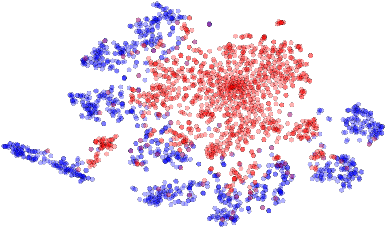
\includegraphics[width=0.45\textwidth]{./figures/adaptation_vis/pool2_mnist2inv_before.pdf}}\hfill%
  \subfigure[Adapted]{%%
    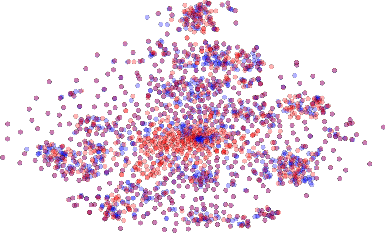
\includegraphics[width=0.45\textwidth]{./figures/adaptation_vis/pool2_mnist2inv_after.pdf}}%%
  \hspace*{\fill}%
  \end{minipage}%
  \begin{minipage}{.5\textwidth}
  \centering
  \small{{\sc Syn Numbers $ \rightarrow $ SVHN}: last hidden layer of the label predictor}
  \setcounter{subfigure}{0}
  \hspace*{\fill}%
  \subfigure[Non-adapted]{%%
    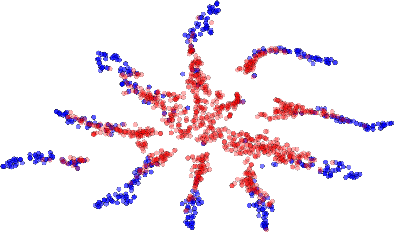
\includegraphics[width=0.45\textwidth]{./figures/adaptation_vis/before.pdf}}\hfill%
  \subfigure[Adapted]{%%
    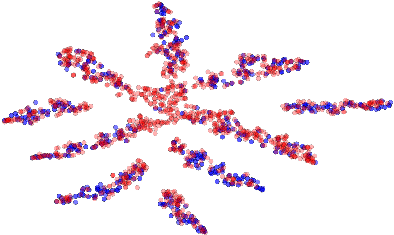
\includegraphics[width=0.45\textwidth]{./figures/adaptation_vis/after.pdf}}%%
  \hspace*{\fill}%
  \end{minipage}
  \caption{The effect of adaptation on the distribution of the extracted features (best viewed in color). The figure shows t-SNE \cite{Maaten13} visualizations of the CNN's activations {\bf (a)} in case when no adaptation was performed and {\bf (b)} in case when our adaptation procedure was incorporated into training. {\it Blue} points correspond to the source domain examples, while {\it red} ones correspond to the target domain. In all cases, the adaptation in our method makes the two distributions of features much closer.}
  \label{fig:exper_adapt_vis}
\end{figure*}

\subsection{Results}
\label{sect:exper_quant}

We now discuss the experimental settings and the results. In each case, we train on the source dataset and test on a different target domain dataset, with considerable shifts between domains (see \fig{exper_domains_examples}). The results are summarized in \tab{results} and \tab{results_office}. 

\vspace{2mm}\noindent {\bf MNIST $ \rightarrow $ MNIST-M.}
Our first experiment deals with the MNIST dataset~\cite{LeCun98} (source). In order to obtain the target domain ({\sc MNIST-M}) we blend digits from the original set over patches randomly extracted from color photos from BSDS500 \cite{Arbelaez11}. This operation is formally defined for two images $ I^{1}, I^{2} $ as $ I_{ijk}^{out} = | I_{ijk}^{1} - I_{ijk}^{2} | $, where $ i, j $ are the coordinates of a pixel and $ k $ is a channel index. In other words, an output sample is produced by taking a patch from a photo and inverting its pixels at positions corresponding to the pixels of a digit. For a human the classification task becomes only slightly harder compared to the original dataset (the digits are still clearly distinguishable) whereas for a CNN trained on MNIST this domain is quite distinct, as the background and the strokes are no longer constant. Consequently, the source-only model performs poorly. Our approach succeeded at aligning feature distributions (\fig{exper_adapt_vis}), which led to successful adaptation results (considering that the adaptation is unsupervised). At the same time, the improvement over source-only model achieved by subspace alignment (SA) \cite{Fernando13} is quite modest, thus highlighting the difficulty of the adaptation task. 

\vspace{2mm}\noindent {\bf Synthetic numbers $ \rightarrow $ SVHN.}
To address a common scenario of training on synthetic data and testing on  real data, we use Street-View House Number dataset {\sc SVHN} \cite{Netzer11} as the target domain and synthetic digits as the source. The latter ({\sc Syn ~Numbers}) consists of ~500,000 images generated by ourselves from Windows fonts by varying the text (that includes different one-, two-, and three-digit numbers), positioning, orientation, background and stroke colors, and the amount of blur. The degrees of variation were chosen manually to simulate SVHN, however the two datasets are still rather distinct, the biggest difference being the structured clutter in the background of SVHN images. 

The proposed backpropagation-based technique works well covering two thirds of the gap between training with source data only and training on target domain data with known target labels. In contrast, SA~\cite{Fernando13} does not result in any significant improvement in the classification accuracy, thus highlighting that the adaptation task is even more challenging than in the case of the MNIST experiment.

\vspace{2mm}\noindent {\bf MNIST $ \leftrightarrow $ SVHN.}
In this experiment, we further increase the gap between distributions, and test on {\sc MNIST} and {\sc SVHN}, which are significantly different in appearance. Training on SVHN even without adaptation is challenging --- classification error stays high during the first 150 epochs. In order to avoid ending up in a poor local minimum we, therefore, do not use learning rate annealing here. Obviously, the two directions ({\sc MNIST} $ \rightarrow $ {\sc SVHN} and {\sc SVHN} $ \rightarrow $ {\sc MNIST}) are not equally difficult. As {\sc SVHN} is more diverse, a model trained on SVHN is expected to be more generic and to perform reasonably on the MNIST dataset. This, indeed, turns out to be the case and is supported by the appearance of the feature distributions. We observe a quite strong separation between the domains when we feed them into the CNN trained solely on { \sc MNIST}, whereas for the {\sc SVHN}-trained network the features are much more intermixed. This difference probably explains why our method succeeded in improving the performance by adaptation in the {\sc SVHN} $ \rightarrow $ {\sc MNIST} scenario (see \tab{results}) but not in the opposite direction (SA is not able to perform adaptation in this case either). Unsupervised adaptation from MNIST to SVHN gives a failure example for our approach (we are unaware of any unsupervised DA methods capable of performing such adaptation).

\vspace{2mm}\noindent {\bf Synthetic Signs $ \rightarrow $ GTSRB.}
Overall, this setting is similar to the {\sc Syn Numbers} $ \rightarrow $ {\sc SVHN} experiment, except the distribution of the features is more complex due to the significantly larger number of classes (43 instead of 10). For the source domain we obtained~100,000 synthetic images (which we call {\sc Syn~Signs}) simulating various photoshooting conditions. Once again, our method achieves a sensible increase in performance once again proving its suitability for the synthetic-to-real data adaptation.

\begin{figure}
  \centering
  \setlength\figureheight{2.7cm}
  \setlength\figurewidth{6.8cm}
  % This file was created by matlab2tikz v0.5.0 running on MATLAB 8.3.
%Copyright (c) 2008--2014, Nico Schlömer <nico.schloemer@gmail.com>
%All rights reserved.
%Minimal pgfplots version: 1.3
%
%The latest updates can be retrieved from
%  http://www.mathworks.com/matlabcentral/fileexchange/22022-matlab2tikz
%where you can also make suggestions and rate matlab2tikz.
%
\begin{tikzpicture}[font=\scriptsize]

\begin{axis}[%
width=0.95092\figurewidth,
height=\figureheight,
at={(0\figurewidth,0\figureheight)},
scale only axis,
xmin=10000,
xmax=50000,
xlabel={Batches seen},
ymin=0,
ymax=1,
ylabel={Validation error},
axis x line*=bottom,
axis y line*=left,
legend style={at={($ (1,1) + (-0.1cm,-0.1cm) $)},anchor=north east,align=left,legend cell align=left,draw=black},
xmajorgrids,
ymajorgrids,
grid style={dashed}
]
\addplot [color=blue,solid,line width=1.0pt]
  table[row sep=crcr]{%
10500	0.199757996632997\\
11000	0.19162984006734\\
11500	0.190788089225589\\
12000	0.192918771043771\\
12500	0.196390993265993\\
13000	0.185527146464646\\
13500	0.190472432659933\\
14000	0.185606060606061\\
14500	0.183422769360269\\
15000	0.189051978114478\\
15500	0.191524621212121\\
16000	0.186079545454545\\
16500	0.179424452861953\\
17000	0.187684132996633\\
17500	0.187868265993266\\
18000	0.180923821548822\\
18500	0.187315867003367\\
19000	0.178661616161616\\
19500	0.18102904040404\\
20000	0.180555555555556\\
20500	0.176662457912458\\
21000	0.183791035353535\\
21500	0.179214015151515\\
22000	0.178898358585859\\
22500	0.178898358585859\\
23000	0.174479166666667\\
23500	0.174742213804714\\
24000	0.171059553872054\\
24500	0.177951388888889\\
25000	0.174794823232323\\
25500	0.174084595959596\\
26000	0.174636994949495\\
26500	0.169034090909091\\
27000	0.171191077441077\\
27500	0.170875420875421\\
28000	0.171506734006734\\
28500	0.170217803030303\\
29000	0.169244528619529\\
29500	0.169875841750842\\
30000	0.168744739057239\\
30500	0.17048085016835\\
31000	0.169454966329966\\
31500	0.167771464646465\\
32000	0.168849957912458\\
32500	0.168323863636364\\
33000	0.168718434343434\\
33500	0.165667087542088\\
34000	0.167376893939394\\
34500	0.169007786195286\\
35000	0.167140151515152\\
35500	0.165667087542088\\
36000	0.167850378787879\\
36500	0.169823232323232\\
37000	0.170691287878788\\
37500	0.16640361952862\\
38000	0.167981902356902\\
38500	0.169875841750842\\
39000	0.166771885521886\\
39500	0.169376052188552\\
40000	0.168087121212121\\
40500	0.165509259259259\\
41000	0.167718855218855\\
41500	0.168060816498317\\
42000	0.166035353535354\\
42500	0.166692971380471\\
43000	0.166429924242424\\
43500	0.167034932659933\\
44000	0.170349326599327\\
44500	0.169744318181818\\
45000	0.168218644781145\\
45500	0.166429924242424\\
46000	0.166324705387205\\
46500	0.168771043771044\\
47000	0.168034511784512\\
47500	0.168718434343434\\
48000	0.171059553872054\\
48500	0.170638678451178\\
49000	0.16819234006734\\
49500	0.168981481481481\\
50000	0.167902988215488\\
};
\addlegendentry{Real data only};

\addplot [color=cyan,solid,line width=1.0pt]
  table[row sep=crcr]{%
10500	0.9625\\
11000	0.79765625\\
11500	0.715625\\
12000	0.6140625\\
12500	0.52109375\\
13000	0.459375\\
13500	0.4484375\\
14000	0.421875\\
14500	0.39453125\\
15000	0.4109375\\
15500	0.34296875\\
16000	0.36875\\
16500	0.3359375\\
17000	0.36171875\\
17500	0.3171875\\
18000	0.3484375\\
18500	0.32421875\\
19000	0.315625\\
19500	0.346875\\
20000	0.31875\\
20500	0.35390625\\
21000	0.3265625\\
21500	0.33359375\\
22000	0.3171875\\
22500	0.28515625\\
23000	0.30546875\\
23500	0.309375\\
24000	0.2796875\\
24500	0.30859375\\
25000	0.30703125\\
25500	0.3078125\\
26000	0.28671875\\
26500	0.2875\\
27000	0.31484375\\
27500	0.2859375\\
28000	0.29375\\
28500	0.31328125\\
29000	0.3078125\\
29500	0.2859375\\
30000	0.2890625\\
30500	0.284375\\
31000	0.2953125\\
31500	0.26953125\\
32000	0.29921875\\
32500	0.30078125\\
33000	0.2640625\\
33500	0.309375\\
34000	0.2734375\\
34500	0.290625\\
35000	0.26796875\\
35500	0.3015625\\
36000	0.26796875\\
36500	0.2921875\\
37000	0.265625\\
37500	0.2765625\\
38000	0.2859375\\
38500	0.32109375\\
39000	0.28046875\\
39500	0.275\\
40000	0.24921875\\
40500	0.29140625\\
41000	0.26640625\\
41500	0.265625\\
42000	0.259375\\
42500	0.2765625\\
43000	0.26796875\\
43500	0.2765625\\
44000	0.27265625\\
44500	0.25546875\\
45000	0.26484375\\
45500	0.271875\\
46000	0.2703125\\
46500	0.26171875\\
47000	0.246875\\
47500	0.25078125\\
48000	0.29609375\\
48500	0.2640625\\
49000	0.26875\\
49500	0.26015625\\
50000	0.2578125\\
};
\addlegendentry{Synthetic data only};

\addplot [color=red,solid,line width=1.0pt]
  table[row sep=crcr]{%
10500	0.943892045454545\\
11000	0.943892045454545\\
11500	0.943892045454545\\
12000	0.943892045454545\\
12500	0.848300715488216\\
13000	0.658722643097643\\
13500	0.590593434343434\\
14000	0.475484006734007\\
14500	0.313946759259259\\
15000	0.235690235690236\\
15500	0.17879313973064\\
16000	0.152383207070707\\
16500	0.12912984006734\\
17000	0.114478114478114\\
17500	0.116214225589226\\
18000	0.1015625\\
18500	0.10066813973064\\
19000	0.101983375420875\\
19500	0.0914351851851852\\
20000	0.0895675505050505\\
20500	0.0894360269360269\\
21000	0.0827283249158249\\
21500	0.0798611111111111\\
22000	0.0859638047138047\\
22500	0.0799137205387205\\
23000	0.0778619528619529\\
23500	0.0737584175084175\\
24000	0.0742582070707071\\
24500	0.0776778198653199\\
25000	0.0771517255892256\\
25500	0.0725747053872054\\
26000	0.0739425505050505\\
26500	0.0734953703703704\\
27000	0.0730744949494949\\
27500	0.0688920454545455\\
28000	0.0702072811447811\\
28500	0.072337962962963\\
29000	0.0670244107744108\\
29500	0.0733638468013468\\
30000	0.0667613636363636\\
30500	0.0692340067340067\\
31000	0.0652093855218855\\
31500	0.0664720117845118\\
32000	0.0655776515151515\\
32500	0.0671296296296296\\
33000	0.0656039562289562\\
33500	0.0646043771043771\\
34000	0.0668665824915825\\
34500	0.0638678451178451\\
35000	0.065077861952862\\
35500	0.0649989478114478\\
36000	0.0672348484848485\\
36500	0.0668665824915825\\
37000	0.0626052188552189\\
37500	0.0652093855218855\\
38000	0.0626315235690236\\
38500	0.0627893518518518\\
39000	0.0613162878787879\\
39500	0.063236531986532\\
40000	0.0629208754208754\\
40500	0.0639467592592593\\
41000	0.0612899831649832\\
41500	0.0653409090909091\\
42000	0.0608691077441077\\
42500	0.0613425925925926\\
43000	0.0630260942760943\\
43500	0.060106271043771\\
44000	0.0638678451178451\\
44500	0.0602377946127946\\
45000	0.0577388468013468\\
45500	0.062684132996633\\
46000	0.0608164983164983\\
46500	0.0603167087542088\\
47000	0.0577651515151515\\
47500	0.0583175505050505\\
48000	0.0591329966329966\\
48500	0.0607112794612795\\
49000	0.0585805976430976\\
49500	0.0583175505050505\\
50000	0.0590540824915825\\
};
\addlegendentry{Both};

\end{axis}
\end{tikzpicture}%
  \caption{Semi-supervised domain adaptation for the traffic signs. As labeled target domain data are shown to the method, it achieves significantly lower error than the model trained on target domain data only or on source domain data only. \vspace{-4mm}}
  \label{fig:exper_semi_test}
\end{figure}

As an additional experiment, we also evaluate the proposed algorithm for semi-supervised domain adaptation, i.e.\ when one is additionally provided with a small amount of labeled target data. For that purpose we split {\sc GTSRB} into the train set (1280 random samples with labels) and the validation set (the rest of the dataset). The validation part is used solely for the evaluation and does not participate in the adaptation. The training procedure changes slightly as the label predictor is now exposed to the target data. \fig{exper_semi_test} shows the change of the validation error throughout the training. While the graph clearly suggests that our method can be used in the semi-supervised setting, thorough verification of semi-supervised setting is left for future work.


\vspace{2mm}\noindent {\bf Office dataset.} 
We finally evaluate our method on {\sc Office} dataset, which is a collection of three distinct domains: {\sc Amazon}, {\sc DSLR}, and {\sc Webcam}. Unlike previously discussed datasets, {\sc Office} is rather small-scale with only 2817 labeled images spread across 31 different categories in the largest domain. The amount of available data is crucial for a successful training of a deep model, hence we opted for the fine-tuning of the CNN pre-trained on the ImageNet \cite{Jia14} as it is done in some recent DA works \cite{Donahue14,Tzeng14,Hoffman14}. We make our approach more comparable with \cite{Tzeng14} by using exactly the same network architecture replacing domain mean-based regularization with the domain classifier.

Following most previous works, we evaluate our method using 5 random splits for each of the 3 transfer tasks commonly used for evaluation. Our training protocol is close to \cite{Tzeng14,Saenko10,Gong12} as we use the same number of labeled source-domain images per category. Unlike those works and similarly to e.g.\ DLID~\cite{Chopra13} we use the whole unlabeled target domain (as the premise of our method is the abundance of unlabeled data in the target domain). Under this transductive setting, our method is able to improve previously-reported state-of-the-art accuracy for unsupervised adaptation very considerably (\tab{results_office}), especially in the most challenging {\sc Amazon} $ \rightarrow $ {\sc Webcam} scenario (the two domains with the largest domain shift).


\section{Conclusion}
\label{sec:discussion}
\section{Discussion}
\label{sec:discussion}

The accuracy on the CKP set shows that the chosen approach is robust, misclassification usually occurs on pictures which are the first few instances of an emotion sequence. Often a neutral facial expression is depicted in those frames. Thus those misclassifications are not necessarily an error in the approach, but in the data selection. Other than that no major problem could be detected. The emotion \textit{Surprise} is often confused with \textit{Disgust} with a rate of 0.045\% which is the highest. Of those images, where an emotion is present, only few are wrongly classified.\\ 


As there is no consent for the misclassified images, they cannot be depicted here. However some unique names are provided. \\
Image S119\_001\_00000010 is classified as \textit{Fear} while the annotated emotion corresponds to \textit{Surprise}. The image depicts a person with a wide open mouth and open eyes. Pictures representing \textit{Surprise} are often very similar, since the persons also have wide open mouths and eyes. In image S032\_004\_00000014 the targeted label \textit{Fear} is confused with \textit{Anger}. While the mouth region in pictures with \textit{Anger} differ, the eye regions are alike, since in both situations the eyes and eyebrows are contracted.\\
Similar effects are experienced when dealing with the MMI Dataset. Since the first two frames are discarded most pictures with neutral positions are excluded. In few images a neutral position can still be found which gives rise to errors. For the same reason as the CKP set images will not be displayed. Due to the approach to extract images of the videos, a unique identifier for the misclassified image cannot be provided.\\
The top confusions are observed for \textit{Fear} and \textit{Surprise} with a rate of 0.0159\% where \textit{Fear} is wrongly misclassified as \textit{Surprise}. Session 1937 shows a woman displaying \textit{Fear} but it is classified as \textit{Surprise}. Both share common features like similar eye and mouth movement. In both emotions, participants move the head slightly backwards. This can be identified by wrinkled skin. The second most confusion rate, \textit{Surprise} being mistaken as \textit{Sadness}, is mostly based on neutral position images. Although the first two images are not used, some selected frames still do not contain an emotion. In Session 1985 \textit{Surprise} is being mistaken as \textit{Sadness}. The image depicts a man with his mouth being slightly curved, making him look sad.\\

DeXpression extracts features and uses them to classify images, but in very few cases the emotions are confused. This happens, as discussed, usually in pictures depicting no emotion. DeXpression performs very well on both tested sets, if an emotion is present.



\balance

{\small
\bibliographystyle{ieee}
\bibliography{paper}
}

\end{document}
